\documentclass[journal]{IEEEtran}
\usepackage{cite}
\usepackage{amsmath,amssymb,amsfonts}
\usepackage{algorithm}
\usepackage{graphicx}
\usepackage{textcomp}
\usepackage{hyperref}
\usepackage{array}
\usepackage{xcolor}
\usepackage{tikz}
\usepackage{algpseudocode}
\usepackage{comment}
\usepackage{enumerate}
\usepackage{booktabs}
\graphicspath{{figures/s41598_final/}}
\begin{document}

\title{AdaptiveSched: Trace-Driven Multi-Objective Cloud Job Scheduling with Performative Reinforcement Learning and Role-Conditioned Actor-Critic Policies}

\author{Suchi Kumari and Dhruv Mishra%
\thanks{Suchi Kumari and Dhruv Mishra are with the Department of Computer Science and Engineering, Shiv Nadar Institution of Eminence, Delhi-NCR, India (e-mail: suchi.singh24@gmail.com; dm409@snu.edu.in).}}

\maketitle

\begin{abstract}
Efficient cloud scheduling requires sequential resource-allocation decisions under competing objectives such as low latency, deadline adherence, fairness, and energy efficiency. This paper studies the problem in a trace-driven setting using Google cluster--style workloads with heterogeneous arrivals, priorities, and resource demands. The scheduler is formulated as a finite-horizon Markov decision process with a transparent five-term reward capturing quality of service, energy use, priority sensitivity, fairness, and overload penalties, thereby enabling controlled algorithmic comparison.

Within this shared environment, we develop two complementary on-policy actor--critic schedulers. \textbf{AdaptiveSched-Base} couples a compact policy-value architecture with performative regularization to improve robustness against policy-induced queue-distribution shift, and is trained with generalized advantage estimation and clipped Proximal Policy Optimization. \textbf{AdaptiveSched-Hybrid} preserves these robustness-oriented design principles while extending the base model through role-conditioned policy heads and queue-dependent mixture weighting to improve specialization under heterogeneous workload conditions.

Experiments follow a reproducible protocol aligned with recent cloud-edge scheduling studies~\cite{zhang2025s41598} and compare against RL-MOTS, HDRL, PPO, A3C, and DQN baselines under a shared benchmark setting. On the validated protocol-normalized Google-derived workload, the base model shows the benefit of performative robustness, and the hybrid model further improves the aggregate operating profile through role-specialized decision making. These findings support queue-shift-aware regularization and state-dependent policy specialization as complementary design principles for trace-driven cloud job scheduling under mixed-priority queues.
\end{abstract}

\begin{IEEEkeywords}
Cloud computing, job scheduling, trace-driven reinforcement learning, multi-objective reward, on-policy actor--critic, PPO, adaptive scheduling, fairness
\end{IEEEkeywords}

\section{\textbf{Introduction}}
Modern cloud and edge computing infrastructures increasingly host a diverse mix of latency-sensitive and throughput-oriented applications within shared resource pools. In such multi-tenant environments, schedulers must make continuous, fine-grained decisions regarding which jobs to execute, defer, or dismiss, while simultaneously balancing service-level agreement (SLA) guarantees against infrastructure efficiency. This balancing act is inherently multi-objective: reducing waiting time and deadline violations may conflict with minimizing energy consumption, while aggressive prioritization of critical workloads can compromise fairness for lower-priority tenants. These trade-offs are further exacerbated under non-stationary workload conditions, where bursty arrivals and evolving job characteristics challenge the assumptions underlying traditional scheduling policies.

Classical scheduling approaches, including queueing-based strategies and heuristic rules, remain widely deployed due to their simplicity and low computational overhead. However, such methods often lack the adaptability required to respond effectively to dynamic workload shifts. In contrast, deep reinforcement learning (DRL) provides a data-driven framework for learning scheduling policies that optimize long-term performance through interaction with the environment. Actor--critic methods, along with policy-optimization techniques such as A3C~\cite{mnih2016asynchronous} and PPO~\cite{schulman2017proximal}, have demonstrated strong empirical performance in complex resource-management settings. Nevertheless, two persistent challenges remain in applying DRL to practical scheduling systems: (i) the lack of transparent and deployment-aligned reward formulations that capture real-world trade-offs, and (ii) limited architectural support for handling heterogeneous priority regimes within shared job queues.

This work addresses these challenges through a principled, implementation-aligned framework. First, we adopt an explicit and decomposable multi-term reward structure that captures key operational objectives, including quality of service, energy efficiency, priority sensitivity, fairness, and overload handling. By fixing this reward design as part of the environment, we enable reproducible comparisons across methods and facilitate clear attribution of performance improvements. Second, we investigate two actor--critic scheduling policies within a shared Markov decision process and trace-driven workload setting: a compact, general-purpose model (\textbf{AdaptiveSched-Base}) and an extended, role-specialized mixture model (\textbf{AdaptiveSched-Hybrid}). The former introduces a performative-regularized learning perspective to improve robustness against queue-distribution shift induced by the scheduler’s own decisions, whereas the latter augments this base with role-conditioned specialization so that robustness and heterogeneous-queue expressiveness are jointly retained.

To ensure methodological clarity and reproducibility, our experimental protocol aligns with recent cloud-edge scheduling benchmarks~\cite{zhang2025s41598}. We adopt synchronized on-policy rollouts, clipped PPO-based updates, and generalized advantage estimation (GAE), thereby avoiding inconsistencies often introduced by asynchronous training assumptions. Comparative evaluation includes RL-MOTS~\cite{zhang2025s41598}, HDRL~\cite{zhang2024hdrl}, PPO, A3C, and DQN under a shared protocol reference, alongside staged ablations that isolate the impact of reward shaping, architectural specialization, and hybridization.

\paragraph{Contributions}
\begin{itemize}
  \item We formulate a unified, trace-driven cloud scheduling environment with an explicit multi-objective reward structure, enabling transparent and reproducible evaluation across algorithms.
  \item We develop \textbf{AdaptiveSched-Base}, a compact actor--critic scheduler that combines reward-aligned action shaping with performative regularization, PPO-style clipped optimization, and generalized advantage estimation to improve robustness against policy-induced queue-distribution shift.
  \item We introduce \textbf{AdaptiveSched-Hybrid}, which extends the base architecture through role-conditioned policy heads for distinct priority regimes and queue-dependent mixture weighting, thereby combining performative robustness with heterogeneous-queue specialization.
  \item We provide a comprehensive evaluation framework with consistent metrics, baseline comparisons, and staged ablation analysis, facilitating clear interpretation of performance gains.
\end{itemize}

The remainder of this paper is organized as follows. Section~\ref{Sec2} reviews related work in cloud scheduling and reinforcement learning. Section~\ref{Sec3} details the problem formulation and proposed methods. Section~\ref{Sec4} presents experimental results and analysis. Section~\ref{Sec5} discusses broader implications and limitations, and Section~\ref{Sec6} concludes the paper.

\begin{table*}[ht]
\centering
\caption{Representative DRL Cloud Scheduling Milestones}
\label{tab:relatedwork}
\small
\setlength{\tabcolsep}{4pt}
\renewcommand{\arraystretch}{1.15}
\begin{tabular}{|>{\centering\arraybackslash}m{2.0cm}|>{\raggedright\arraybackslash}m{3.0cm}|>{\raggedright\arraybackslash}m{6cm}|>{\raggedright\arraybackslash}m{5.6cm}|}
\hline
\textbf{Year} & \textbf{Reference} & \textbf{Main contribution} & \textbf{Residual limitation relative to AdaptiveSched} \\ \hline
2009--2010 & Isard \textit{et al.}, Zaharia \textit{et al.}~\cite{isard2009quincy, zaharia2010delay} & Introduced data-aware and fairness-aware cluster scheduling principles for shared compute workloads. & Policy logic remains heuristic and brittle under non-stationary multi-objective trade-offs. \\ \hline
2011--2012 & Hindman \textit{et al.}, Ghodsi \textit{et al.}, Calheiros \textit{et al.}~\cite{hindman2011mesos, ghodsi2011drf, calheiros2011cloudsim} & Established cluster resource arbitration and reproducible cloud simulation infrastructure. & Lacks learned sequential control that adapts online to shifting queue composition. \\ \hline
2012--2016 & Beloglazov \textit{et al.}, Schwarzkopf \textit{et al.}, Ousterhout \textit{et al.}, Verma \textit{et al.}, Burns \textit{et al.}~\cite{beloglazov2012energy, schwarzkopf2013omega, ousterhout2013sparrow, verma2015borg, burns2016borg} & Scalable multi-scheduler and production orchestration architectures with stronger energy-management awareness. & Strong systems engineering, but limited explicit multi-objective RL policy optimization. \\ \hline
2013--2014 & Delimitrou and Kozyrakis, Grandl \textit{et al.}~\cite{delimitrou2013paragon, delimitrou2014quasar, grandl2014tetris} & Interference-aware and multi-resource-aware scheduling with improved packing/utilization. & Performance-sensitive heuristics require frequent retuning under workload drift. \\ \hline
2016 & Mao \textit{et al.}~\cite{mao2016resource} & DeepRM established DRL as a viable scheduler for multi-resource cluster jobs. & Early single-policy design; limited fairness/priority decomposition and narrow reward transparency. \\ \hline
2017--2019 & Decima and related works~\cite{decima2019} & Extended RL toward DAG-aware scheduling with richer task structure. & Focused workloads and specialized objectives reduce direct comparability across cloud job regimes. \\ \hline
2020--2022 & Survey and structure-building phase~\cite{arunarani2019survey, zhou2022selector, zhou2024aireview} & Consolidated objective design and introduced hierarchical DRL selector logic for cloud resource scheduling. & Still limited apples-to-apples policy-architecture comparison under fixed trace/reward protocols. \\ \hline
2023 & Xiu \textit{et al.}, Wang \textit{et al.}~\cite{xiu2023mrlcc, wang2023erlfc} & Added meta-RL adaptation and sustainability-aware RL scheduling in cloud settings. & Improvements are task-specific; controlled head-to-head architectural isolation remains limited. \\ \hline
2024 & Cheng \textit{et al.}, Zhang \textit{et al.}, Mangalampalli \textit{et al.}~\cite{cheng2024preemptive, zhang2024hdrl, mangalampalli2024efficient} & Advanced preemptive DRL scheduling, hierarchical policy structure, and efficient multi-cloud DRL deployment. & Strong method gains, but limited unified evaluation of queue-shift robustness plus role-specialized actor-critic decomposition. \\ \hline
2025 & Zhang \textit{et al.}~\cite{zhang2025s41598} & Multi-objective cloud-edge scheduling with publication-grade reporting templates. & Stronger metric reporting, but still limited emphasis on policy interference across mixed-priority queue regimes. \\ \hline
\textbf{Proposed Work} & \textbf{AdaptiveSched} & Shared trace-driven MDP, transparent five-term reward, performative-regularized base scheduling, and role-conditioned hybrid scheduling under one PPO/GAE backbone. & Targets the remaining gap: reproducible comparison of queue-shift-aware and role-specialized actor--critic schedulers under heterogeneous priority dynamics. \\ \hline
\end{tabular}
\end{table*}

\section{\textbf{Related Work}} \label{Sec2}
The evolution of cloud job scheduling can be read as a sequence of attempts to bridge \emph{static allocation logic} and \emph{dynamic service objectives}. Early work emphasized heuristic and data-aware scheduling under shared infrastructure~\cite{isard2009quincy, zaharia2010delay, armbrust2010view}. In parallel, production-oriented resource sharing and fairness abstractions (Mesos/DRF) and cloud simulation toolchains established foundational system and evaluation practices~\cite{hindman2011mesos, ghodsi2011drf, calheiros2011cloudsim}. These contributions defined the operating context but remained hand-designed, so retuning under workload shift was costly.

The next phase added scalable systems control and interference-aware optimization. Energy-aware consolidation and multi-scheduler coordination improved utilization and operational efficiency at scale~\cite{beloglazov2012energy, schwarzkopf2013omega, ousterhout2013sparrow, verma2015borg, burns2016borg}. Resource-interference-aware schedulers further improved placement quality~\cite{delimitrou2013paragon, delimitrou2014quasar}. However, these methods still relied on engineered policies. DRL then became a viable sequential scheduler, with DeepRM as a key transition showing that dispatch policies can be learned from interaction~\cite{mao2016resource}, later expanded by actor-critic optimization methods~\cite{mnih2016asynchronous, schulman2017proximal}.

From 2019 onward, the focus shifted from feasibility to policy structure and comparability. Decima introduced richer graph-informed scheduling policies~\cite{decima2019}. Subsequent work expanded to hierarchical selector policies~\cite{zhou2022selector}, meta-RL adaptation and sustainability-aware scheduling~\cite{xiu2023mrlcc, wang2023erlfc}, and preemptive or efficient DRL schedulers in multi-cloud settings~\cite{cheng2024preemptive, mangalampalli2024efficient}. Recent hierarchical DRL and cloud-edge RL studies further improved structural expressiveness and reporting discipline~\cite{zhang2024hdrl, zhang2025s41598}. At the same time, survey-driven synthesis highlighted unresolved issues in state design, convergence stability, and deployment realism~\cite{zhou2024aireview}. The remaining gap is controlled comparison: fixed trace/reward protocol with explicit isolation of queue-shift robustness and role specialization effects.

The most recent literature, especially in 2024--2025, shows a clear transition from generic DRL scheduling toward more specialized and reporting-aware schedulers~\cite{zhou2024aireview, zhang2025s41598}. This recent generation fills several earlier gaps: workloads are more heterogeneous, objectives are more realistic, and evaluation reporting is usually richer. However, the new papers also expose a remaining inconsistency. Some focus on SLA risk, others on cost-energy trade-offs, others on heterogeneous clusters, and others on framework-specific environments. As a result, the literature still lacks a unified trace-driven comparison in which transparent multi-objective reward design, priority-sensitive queue dynamics, and policy-architecture specialization are studied together under a shared evaluation protocol.

Among recent studies, the closest benchmark anchor is Zhang and Ou~\cite{zhang2025s41598}, which provides a comparable cloud-edge framing and metric template (makespan, energy, cost, waiting, violation). This manuscript follows that comparative discipline but differs in two implementation-critical ways: it enforces a single synchronized PPO/GAE training stack for all variants, and it evaluates both a performative-regularized base policy and a role-conditioned hybrid policy under the same trace/reward protocol. The staged ablations are intended to isolate these policy-side effects rather than introduce a new environment definition.

Viewed chronologically, the cumulative research trajectory is therefore clear. Heuristics solved tractability; DRL solved adaptability; hierarchical and hybrid policies improved structural expressiveness; recent multi-objective and SLA-aware schedulers improved realism. The remaining gap is the joint treatment of four requirements in one reproducible framework: \emph{trace realism}, \emph{transparent reward decomposition}, \emph{policy robustness under mixed-priority queue regimes}, and \emph{implementation-aligned ablation against standard actor--critic baselines}. That is the point of departure for the present work.

\subsection*{Baseline paper alignment}
The reporting structure and metric set (makespan, energy, cost, waiting time, and violation rate) follow the Scientific Reports RL-MOTS benchmark template~\cite{zhang2025s41598}. For hierarchical comparison, the manuscript anchors HDRL to the Applied Soft Computing formulation~\cite{zhang2024hdrl}. The present manuscript extends this baseline set through implementation-aligned actor--critic modeling, trace-driven comparison of two policy variants, and model-specific ablations for AdaptiveSched-Base and AdaptiveSched-Hybrid.

\section{Research Gap} \label{sec:gap}
The chronological review above shows that the field has progressed by filling gaps one layer at a time, but not yet in an integrated manner. Early heuristics addressed feasible allocation but lacked adaptivity; DRL addressed adaptivity but often used opaque reward functions; hierarchical and hybrid designs improved structural flexibility but were frequently evaluated in specialized or partially comparable environments; the latest SLA-aware and multi-objective schedulers improved realism, yet usually optimize one dominant concern at a time (e.g., SLA risk, energy, workflow delay, or cluster load). Consequently, the current research gap is \emph{integrative}: there is still limited evidence on how a transparent, multi-term reward environment interacts with different actor--critic policy structures under the same trace-driven cloud workload.

Three concrete limitations follow from this gap. First, many papers conflate environment design with algorithmic contribution, making it difficult to determine whether observed gains arise from better reward engineering, better state design, or a better policy architecture. Second, most schedulers still represent heterogeneous queues with a single policy head or platform-specific controller, despite the fact that practical traces mix low-priority background jobs, medium-priority throughput jobs, and high-priority latency-sensitive jobs that can induce conflicting training gradients. Third, comparative reporting is often fragmented across platforms, datasets, and metric definitions, which weakens cumulative understanding even as the number of DRL schedulers grows.

This work addresses those limitations by fixing the environment and varying the policy structure in a controlled way. Specifically, we define a shared trace-driven MDP and a transparent five-term reward that separately captures QoS, energy, priority satisfaction, fairness, and dismissal penalties. On top of this common environment, we compare a performative-regularized actor--critic base model and a role-conditioned hybrid extension. Because both variants use the same traces, reward, and evaluation pipeline~\cite{reiss2011googlecluster, zhang2025s41598}, differences in performance can be interpreted as methodological rather than environmental. In this sense, the paper is intended not merely as another DRL scheduler, but as an implementation-aligned step toward more cumulative and comparable cloud scheduling research in which queue-shift robustness and policy specialization are treated as complementary contributions.

\section{\textbf{Proposed Approach}} \label{Sec3}

\subsection{Problem formulation}
The scheduling problem considered in this work is a constrained sequential decision problem defined over a shared cloud cluster serving heterogeneous jobs with priorities, deadlines, and multi-resource demands. At each decision epoch, the scheduler must select which queued job to dispatch next under limited CPU and memory capacity while accounting for both immediate service effects and longer-horizon queue evolution. The formulation must therefore capture four interacting properties: trace-driven arrivals, resource-feasibility constraints, priority-sensitive service differentiation, and long-horizon multi-objective optimization. These requirements motivate the system model and MDP formalization given below.

\subsection{System model and decision-process formulation}
We model scheduling as a finite-horizon Markov decision process
\begin{equation}
\mathcal{M} = (\mathcal{S}, \mathcal{A}, P, r, \gamma, H)
\end{equation}
where $\mathcal{S}$ is the state space, $\mathcal{A}$ is the action space, $P(s_{t+1}\mid s_t,a_t)$ denotes the trace-driven transition kernel induced by job arrivals and simulator dynamics, $r$ is the scalar reward, $\gamma \in (0,1)$ is the discount factor, and $H$ is the horizon for one rollout segment. Exogenous arrivals are obtained from Google cluster--style traces~\cite{reiss2011googlecluster} after protocol normalization. At each decision step $t$, the scheduler observes the current queue state, dispatches at most one admissible job, receives an immediate multi-objective reward, and transitions to the next simulator state.

\paragraph{System model}
Consider a cluster with $M$ execution units (servers, workers, or VMs) indexed by $m \in \{1,\dots,M\}$. Each unit has finite capacity vector
\begin{equation}
c_m = \left[c_m^{cpu}, c_m^{mem}\right] \in \mathbb{R}_{+}^{2}
\end{equation}
and the aggregate cluster capacity is
\begin{equation}
C = \sum_{m=1}^{M} c_m
\end{equation}
Each queued job $j$ is characterized by demand vector
\begin{equation}
d_j = \left[d_j^{cpu}, d_j^{mem}\right]
\end{equation}
arrival time $a_j$, estimated service requirement $C_j$, deadline $d\ell_j$, and priority score $\mathcal{P}_j$. Let $u_t=[u_t^{cpu},u_t^{mem}]$ denote currently committed resources. A dispatch action is feasible only if
\begin{equation}
u_t + d_j \preceq C
\label{eq:feasibility}
\end{equation}
where $\preceq$ denotes componentwise inequality. If Eq.~\eqref{eq:feasibility} does not hold, the job cannot be started immediately and must remain queued unless the environment applies overload control. The waiting set, active set, and completed set evolve according to job arrivals, dispatches, completions, and dismissals. This system model makes clear that the scheduler is not merely ranking jobs: it is solving a constrained sequential allocation problem under dynamic multi-resource capacity limits.

\paragraph{Assumptions}
The formulation relies on a small number of explicit assumptions that are consistent with the implemented simulator. First, trace arrivals are exogenous and not controllable by the scheduler. Second, the scheduler selects at most one queue action per decision epoch from a bounded visible queue window. Third, job resource demands are treated as known normalized inputs at scheduling time, while realized queue evolution remains stochastic because of trace arrivals and completions. Fourth, overload handling is part of the environment rather than a learned auxiliary controller. These assumptions are important because they delimit the scope of the policy: AdaptiveSched learns dispatch behavior under constrained capacity and trace non-stationarity, not workload forecasting or autoscaling policy.

\begin{table*}[t]
\centering
\caption{Core Symbols in Proposed Formulation}
\label{tab:symbols}
\small
\begin{tabular}{@{}p{3.5cm}p{4.9cm}p{9.5cm}@{}}
\toprule
\textbf{Symbol} & \textbf{Meaning} & \textbf{Default value / role} \\
\midrule
$\mathcal{M}=(\mathcal{S},\mathcal{A},P,r,\gamma,H)$ & Finite-horizon scheduling MDP & Core problem model; standard RL notation~\cite{sutton1998reinforcement} \\
$c_m$ & Capacity vector of execution unit $m$ & $[c_m^{cpu}, c_m^{mem}]$; multi-resource cluster convention~\cite{mao2016resource, ghodsi2011drf} \\
$s_t$ & Scheduler state at time $t$ & Queue + system summary state \\
$R_t$ & Composite scalar reward & Weighted sum of 5 terms \\
$w_1,\ldots,w_5$ & Reward weights & Normalized such that $\sum_i w_i = 1$; standard scalarization form~\cite{zhan2015survey} \\
$\gamma$ & Discount factor & $(0,1)$; standard return discounting~\cite{sutton1998reinforcement} \\
$\lambda$ & GAE parameter & GAE smoothing parameter~\cite{schulman2017proximal} \\
$\epsilon$ & PPO clip parameter & PPO clipping parameter~\cite{schulman2017proximal} \\
$\lambda_{\text{perf}}$ & Performative regularization weight & Fixed nonzero Base regularization strength~\cite{perdomo2020performative, mandal2023performative} \\
$w_t^{low},w_t^{med},w_t^{high}$ & Role-mixture weights in Hybrid & Softmax-normalized, sum to 1 \\
\bottomrule
\end{tabular}
\end{table*}

\paragraph{State space}
Let $\mathcal{Q}_t = \{j_1,\ldots,j_{K_t}\}$ denote the visible queue at time $t$, truncated or padded to a fixed scheduler window $K$. Each job $j$ is represented by a feature vector
\begin{equation}
x_j = [\hat{a}_j,\hat{c}_j,\hat{u}^{cpu}_j,\hat{u}^{mem}_j,\hat{p}_j,\hat{d}_j,\hat{\delta}_j] \in \mathbb{R}^{d_j},
\end{equation}
where $\hat{a}_j$ is normalized arrival time, $\hat{c}_j$ normalized runtime/compute demand, $\hat{u}^{cpu}_j$ and $\hat{u}^{mem}_j$ normalized CPU and memory requirements, $\hat{p}_j$ normalized priority, $\hat{d}_j$ normalized deadline, and $\hat{\delta}_j$ deadline slack. In addition to per-job attributes, the state includes queue-level and system-level summaries:
\begin{equation}
g_t = [\rho_t^{cpu}, \rho_t^{mem}, \bar{p}_t, h_t^{prio}, \bar{\delta}_t, \bar{w}_t, n_t^{active}, n_t^{wait}] \in \mathbb{R}^{d_g}
\end{equation}
where $\rho_t^{cpu}$ and $\rho_t^{mem}$ denote current utilization, $h_t^{prio}$ is a priority histogram or composition summary, $\bar{w}_t$ is the average waiting profile, and $n_t^{active},n_t^{wait}$ summarize cluster occupancy. The final state is
\begin{equation}
s_t = \Big[g_t,\; x_{j_1},\ldots,x_{j_K}\Big] \in \mathbb{R}^{d_s}
\end{equation}
This representation is rich enough to encode urgency, resource pressure, and priority composition, while still allowing bounded neural inference.

\paragraph{Action space and feasibility masking}
The scheduler selects one queue slot from the visible queue window:
\begin{equation}
\mathcal{A}_t = \{1,\ldots,K\}
\end{equation}
where each action indexes one visible queue slot. Since not every queue position corresponds to a feasible dispatch, we define a binary feasibility mask
\begin{equation}
m_t(a) \in \{0,1\}
\end{equation}
with $m_t(a)=1$ iff action $a$ corresponds to a valid and currently dispatchable job. The policy therefore operates over masked logits,
\begin{equation}
\tilde{\ell}_t(a) =
\begin{cases}
\ell_t(a), & m_t(a)=1\\
-\infty, & m_t(a)=0
\end{cases}
\end{equation}
so that inadmissible queue slots receive zero sampling probability. This formalization ensures that policy learning focuses on ranking feasible candidate jobs rather than implicitly learning simulator invalidity rules.

\paragraph{Transition dynamics}
Given $(s_t,a_t)$, the simulator dispatches the selected job if capacity permits, updates active executions, processes completions, admits newly arrived jobs from the trace, and applies overload handling when necessary. Thus
\begin{equation}
s_{t+1} \sim P(\cdot \mid s_t, a_t)
\end{equation}
is partly endogenous (through dispatch choice) and partly exogenous (through trace arrivals and job completions). This combination makes the scheduling problem non-stationary from the policy’s perspective, which is precisely why robust and structured policy representations are necessary.

\subsection{Composite reward and environment design}
The scalar reward is specified at the environment level and shared across all compared algorithms. This decision is central to the paper: it fixes the optimization target so that differences between methods can be attributed to policy architecture and learning dynamics rather than to hidden reward changes.
\begin{equation}
R_t = w_1 R_t^{QoS} + w_2 R_t^{\mathcal{E}} + w_3 R_t^{\mathcal{P}} + w_4 R_t^{\mathcal{F}} + w_5 R_t^{\mathcal{D}} \label{eq:reward}
\end{equation}
Weights $w_1,\ldots,w_5$ satisfy $\sum_i w_i=1$ and define a transparent scalarization policy. While adaptive weighting can improve preference responsiveness~\cite{mao2016resource}, fixed weighting is intentionally retained here to isolate algorithmic effects from objective drift. The component definitions are retained as follows: QoS via latency ratio~\eqref{eq:QoSreward}--\eqref{eq:latency}; energy via~\eqref{eq:energyreward}, \eqref{eq:energyjob}, and~\eqref{eq:iota}; priority via~\eqref{eq:priorityreward}; fairness via~\eqref{eq:rewardfairness}; and dismissal penalty via~\eqref{eq:rewarddismissal}. Together, these terms encourage the agent to avoid myopic throughput optimization that can otherwise amplify unfairness or deadline misses.
\begin{equation}
R_t^{QoS} = 1 - \frac{L_j}{L_{\max}} \label{eq:QoSreward}
\end{equation}
\begin{equation}
L_j = T^{wait}_j + T^{queue}_j + T^{exec}_j \label{eq:latency}
\end{equation}
with execution time model $T^{exec}_j = C_j / (f (1 - \theta_j))$ (parameters as in the environment).
\begin{equation}
R_t^{\mathcal{E}} = -\alpha \times \mathcal{E}_j \label{eq:energyreward}
\end{equation}
\begin{equation}
\mathcal{E}_j = \left( \mathcal{W}_{\text{base}} + U^{CPU} \times \iota \times (\mathcal{W}_{\text{max}} - \mathcal{W}_{\text{base}}) \right) \times \tau \label{eq:energyjob}
\end{equation}
\begin{equation}
\iota = \text{CPI} \times z + \text{MAPI} \times (1 - z) \label{eq:iota}
\end{equation}
\begin{equation}
R_t^{\mathcal{P}} = \mathcal{P}_j (1 - L_j) \label{eq:priorityreward}
\end{equation}
\begin{equation}
R_t^{\mathcal{F}} = -\lambda\, \sigma^2(U^{Resource}) \label{eq:rewardfairness}
\end{equation}
\begin{equation}
R_t^{\mathcal{D}} = -\mu\, D_t \label{eq:rewarddismissal}
\end{equation}
The reward can also be interpreted as a constrained scalarization of five operational desiderata: service quality, energy sensitivity, priority alignment, resource fairness, and overload robustness. In practical terms, $R_t^{QoS}$ rewards decisions that reduce end-to-end delay, $R_t^{\mathcal{E}}$ discourages energy-expensive allocations, $R_t^{\mathcal{P}}$ preserves priority-aware service differentiation, $R_t^{\mathcal{F}}$ discourages extreme imbalance in resource usage, and $R_t^{\mathcal{D}}$ explicitly prices overload-induced dismissals. This decomposition is important because the later ablation and architectural comparisons depend on a stable reward reference.

\paragraph{Reward-aligned shaping}
Reward-aligned shaping is used at the policy interface to encode urgency and priority signals directly in action logits before sampling:
\begin{equation}
\mathcal{P}(a_t = j) = \frac{e^{{(Q(s_t,j) + \beta \mathcal{P}_j)}}}{\sum_k e^{{(Q(s_t,k) + \beta \mathcal{P}_k)}}} \label{eq:softmax}
\end{equation}
where $Q(s_t,j)$ denotes the pre-shaping policy preference score and $\beta$ controls the strength of priority-sensitive biasing. More generally, we can write the shaped logit for action $j$ as
\begin{equation}
\ell_t^{shape}(j) = \ell_t(j) + \beta_p \hat{p}_j + \beta_u u_j + \beta_f f_j
\end{equation}
where $u_j$ is an urgency statistic (e.g., inverse slack) and $f_j$ is a fairness-related corrective term. This shaping is not itself a replacement for policy learning; rather, it acts as a structured inductive bias that improves action discrimination in congested states.

\paragraph{Overload handling}
When utilization exceeds a predefined threshold, the environment applies a controlled victim-selection mechanism that dismisses the lowest-priority jobs until resource pressure returns below the limit. Algorithm~\ref{alg:victim} specifies this rule and links dismissal count directly to the penalty term $D_t$. This explicit overload model reflects practical admission-control behavior and prevents hidden simulator effects from confounding policy comparisons.

\begin{algorithm}[ht]
\caption{Victim Selection Under Overload Rule}
\label{alg:victim}
\begin{algorithmic}[1]
\State \textbf{Input:} Job queue $Q_t$, priority set $\mathcal{P}_t$, threshold $T_{\max}$
\If{Resource usage $> T_{\max}$}
  \State Sort $Q_t$ by ascending $\mathcal{P}_j$
  \While{Resource usage $> T_{\max}$}
    \State Remove lowest-priority job; $\mathcal{D}_t \leftarrow \mathcal{D}_t + 1$
  \EndWhile
\EndIf
\end{algorithmic}
\end{algorithm}

\subsection{Chronological model development: from base to hybrid}
The proposed methodology was not developed as a single monolithic design. Instead, it emerged through a staged process motivated by implementation findings on increasingly realistic queue states. We first constructed the trace-driven environment defined above and trained a compact on-policy actor--critic policy, which we denote as \textbf{AdaptiveSched-Base}. This base model was intentionally simple: one encoder, one policy head, one value head, and a transparent reward function. Its purpose was to establish a strong, implementation-aligned reference model under the exact simulator used throughout the paper.

During early development, the base model was designed to solve one of the central methodological problems of trace-driven scheduling: the scheduler’s own policy changes the future queue distribution that it will later face. We therefore equipped the base learner with a performative regularization term so that queue-shift robustness became a first-class contribution rather than an incidental add-on. At the same time, experiments with the performative-regularized base model exposed three remaining weaknesses. First, a single policy head was still required to represent conflicting scheduling preferences across low-, medium-, and high-priority regimes, which increased policy interference. Second, high-pressure queue states often required sharper distinctions between urgency-sensitive and throughput-oriented decisions than a monolithic policy could stably express. Third, performative robustness improved stability under distribution shift, but it did not by itself resolve representational coupling between priority regimes. These observations motivated the transition to \textbf{AdaptiveSched-Hybrid}, which preserves the robustness-oriented logic of the base model while adding role-conditioned specialization and state-dependent mixing. The staged ablation analysis later in this section follows exactly this design trajectory: base actor--critic $\rightarrow$ performative-regularized base $\rightarrow$ shaping $\rightarrow$ role mixture $\rightarrow$ full hybrid.

\subsection{AdaptiveSched-Base: generalist actor--critic scheduler}
AdaptiveSched-Base is the first implemented policy family and serves as the generalist reference architecture. It uses a shared multilayer perceptron encoder $h_t = f_\psi(s_t)$, followed by a policy head and value head:
\begin{equation}
\ell_t = W_\pi h_t + b_\pi,\qquad V_\phi(s_t) = W_V h_t + b_V
\end{equation}
The resulting policy is a masked categorical distribution
\begin{equation}
\pi_\theta(a_t \mid s_t) = \text{Categorical}(\text{softmax}(\tilde{\ell}^{shape}_t))
\end{equation}
where $\tilde{\ell}^{shape}_t$ includes feasibility masking and reward-aligned shaping. The value function estimates the expected discounted return,
\begin{equation}
V^\pi(s_t) = \mathbb{E}_\pi \left[\sum_{l=0}^{H-t-1}\gamma^l R_{t+l}\;\middle|\; s_t \right]
\end{equation}

\paragraph{GAE and PPO objective}
Training proceeds through mini-batch on-policy rollouts. Temporal-difference residuals are computed as
\begin{equation}
\delta_t = R_t + \gamma V_\phi(s_{t+1}) - V_\phi(s_t)
\end{equation}
and generalized advantage estimates are
\begin{equation}
\hat{A}_t = \sum_{l=0}^{H-t-1}(\gamma\lambda)^l \delta_{t+l}
\end{equation}
Let
\begin{equation}
r_t(\theta) = \frac{\pi_\theta(a_t\mid s_t)}{\pi_{\theta_{\text{old}}}(a_t\mid s_t)}
\end{equation}
be the PPO probability ratio. The clipped surrogate objective is
\begin{equation}
\mathcal{L}_{\text{PPO}}(\theta) =
\mathbb{E}_t\left[
\min\left(
r_t(\theta)\hat{A}_t,\;
\text{clip}(r_t(\theta),1-\epsilon,1+\epsilon)\hat{A}_t
\right)
\right]
\end{equation}
The full optimization objective for the base model is
\begin{equation}
\mathcal{J}_{base}
=
\mathcal{L}_{\text{PPO}}
- c_v \mathcal{L}_{value}
+ c_e \mathcal{H}(\pi_\theta)
- \lambda_{\text{perf}}\mathcal{L}_{perf}
\end{equation}
where $\mathcal{L}_{value}=\mathbb{E}_t[(V_\phi(s_t)-\hat{G}_t)^2]$, $\mathcal{H}(\pi_\theta)$ is policy entropy, and $\mathcal{L}_{perf}$ is the performative regularizer based on a queue-shift proxy.

\paragraph{Performative regularization as a core contribution}
The performative term is used to model the fact that the scheduler changes its own future data distribution through its current dispatch decisions. This is aligned with performative learning, where the deployed decision rule affects the population or state distribution on which it is later evaluated~\cite{perdomo2020performative,mandal2023performative}. In the present setting, a policy that repeatedly favors certain job types can alter future queue composition, waiting profiles, and congestion patterns, thereby changing the distribution of states encountered during subsequent rollouts. Thus, the regularizer is not intended as a generic smoothness penalty; rather, it is a scheduling-specific surrogate for policy-induced state-distribution shift in a sequential environment. We capture this effect through a queue-shift proxy
\begin{equation}
\Delta_t = \| \varphi(s_{t+1}) - \varphi(s_t) \|_2^2
\end{equation}
where $\varphi(\cdot)$ denotes a low-dimensional queue-statistics map, for example over priority composition, average slack, and load profile. If the scheduler induces abrupt changes in this summary, then the rollout distribution used for subsequent optimization can drift away from the regime under which the current gradient estimate is reliable. The performative regularizer can then be written in generic form as
\begin{equation}
\mathcal{L}_{perf} = \mathbb{E}_t[\Delta_t]
\end{equation}
or, more generally, as a discrepancy between consecutive induced queue-distribution summaries. The role of $\lambda_{\text{perf}}$ is therefore to penalize policy updates that improve immediate return at the cost of destabilizing the future queue distribution. In this sense, the base objective approximates a performatively aware policy update: PPO still maximizes long-horizon return, but the additional penalty discourages solutions that create self-induced queue regimes with poorer downstream controllability. This component is one of the core contributions of the paper because it explicitly addresses the feedback loop between scheduling policy and subsequent workload context, a phenomenon that is often present but rarely modeled directly in trace-driven scheduling studies.

\paragraph{Why the base model still required extension}
AdaptiveSched-Base is already a meaningful contribution because it combines a transparent reward, structured shaping, stable on-policy optimization, and performative robustness against queue-shift effects. However, its representational bias is still monolithic. A single policy head must learn to rank backlog-clearing actions, fairness-preserving actions, and deadline-critical actions under one shared parameterization. In exploratory runs, this produced two technical symptoms: (i) unstable preference switching when queue composition changed abruptly, and (ii) insufficient separation between medium-priority throughput decisions and high-priority urgency decisions. These observations did not invalidate the base contribution; rather, they revealed that robustness to policy-induced distribution shift and specialization across queue regimes are distinct needs. This insight motivated the transition to a role-specialized hybrid architecture.

\begin{figure}[t]
\centering
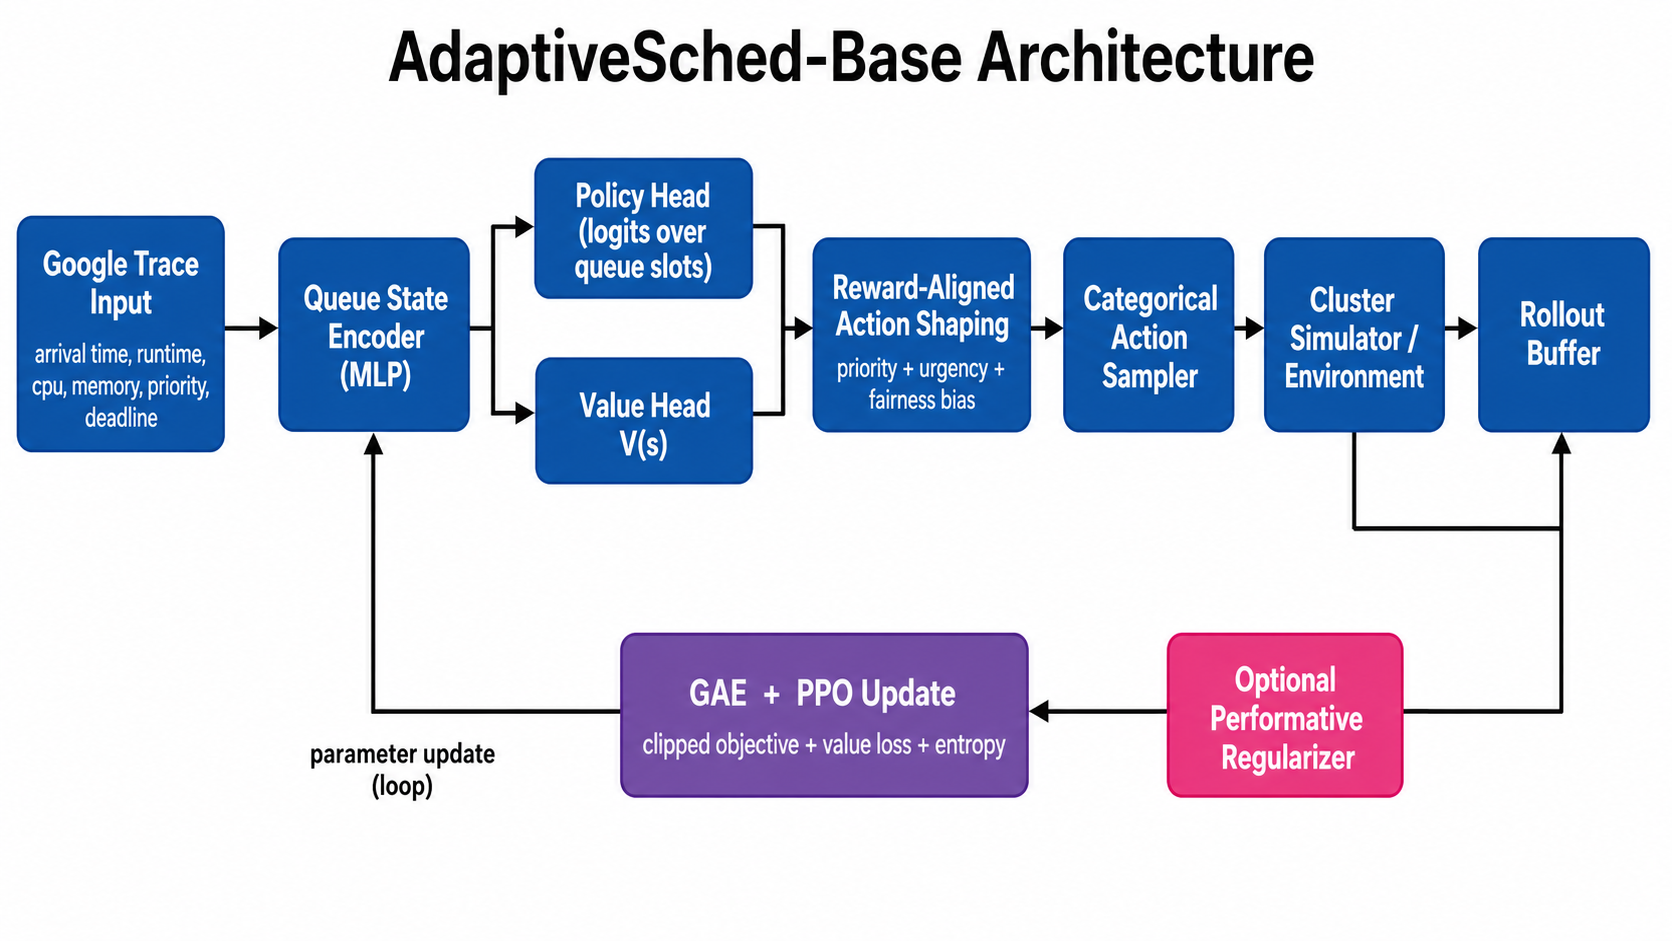
\includegraphics[width=\columnwidth]{figures/s41598_final/BaseArch.png}
\caption{AdaptiveSched-Base Architecture}
\label{fig:base_arch}
\end{figure}

Figure~\ref{fig:base_arch} visualizes the exact computational pathway of the base scheduler. The important point is that all job contexts, regardless of urgency or priority regime, are compressed into one shared latent representation before a single policy head produces dispatch preferences, while performative regularization controls the extent to which current decisions induce undesirable future queue shifts. This architectural compactness makes the base model computationally efficient and methodologically clean, which is why it serves as both a standalone contribution and the starting point of the design progression. At the same time, the figure also makes the central limitation visible: the model has no explicit mechanism for separating backlog-oriented and deadline-oriented control signals once they are embedded in the same policy pathway.

\begin{algorithm}[t]
\caption{AdaptiveSched-Base Training with Masked PPO}
\label{algo:base}
\begin{algorithmic}[1]
\State \textbf{Input:} trace segments $\mathcal{T}$, horizon $H$, clip $\epsilon$, GAE $\lambda$, discount $\gamma$
\State Initialize encoder $\psi$, policy parameters $\theta$, value parameters $\phi$
\For{update $k=1,2,\ldots,K_{\max}$}
  \State Reset simulator with next trace segment $\tau \sim \mathcal{T}$
  \State Initialize rollout buffer $\mathcal{B}\leftarrow \emptyset$
  \For{$t=1$ to $H$}
    \State Observe state $s_t=[g_t,x_{j_1},\ldots,x_{j_K}]$
    \State Compute hidden embedding $h_t \leftarrow f_\psi(s_t)$
    \State Compute raw logits $\ell_t$ and value estimate $V_\phi(s_t)$
    \State Build feasibility mask $m_t$ from current queue and capacity
    \State Compute shaped logits $\ell_t^{shape}$ using priority/urgency/fairness bias
    \State Mask inadmissible actions and sample $a_t \sim \pi_\theta(\cdot\mid s_t)$
    \State Execute $a_t$ in simulator, receive $R_t$, $s_{t+1}$, done flag
    \State Keep environment reward fixed and store queue-shift proxy for optimizer-side regularization
    \State Store $(s_t,a_t,R_t,V_\phi(s_t),\log \pi_\theta(a_t\mid s_t),done)$ in $\mathcal{B}$
    \If{done} \State \textbf{break} \EndIf
  \EndFor
  \State Compute bootstrap returns $\hat{G}_t$ and GAE advantages $\hat{A}_t$ from $\mathcal{B}$
  \For{each optimization epoch}
    \State Re-evaluate logits, values, and action log-probabilities on mini-batches from $\mathcal{B}$
    \State Compute PPO surrogate, value loss, entropy bonus, and performative regularization term
    \State Update $(\psi,\theta,\phi)$ by gradient ascent on $\mathcal{J}_{base}$
  \EndFor
\EndFor
\end{algorithmic}
\end{algorithm}

\subsection{From performative robustness to AdaptiveSched-Hybrid}
The main hypothesis behind AdaptiveSched-Hybrid is that mixed-priority queues induce a latent mixture of scheduling regimes. In one regime, the scheduler should primarily protect deadlines; in another, it should improve utilization and queue clearance; in a third, it should maintain fairness and avoid starvation. If these regimes are compressed into a single policy head, the resulting gradients can interfere. We therefore introduce role-conditioned decomposition while keeping the same environment, action interface, PPO backbone, and performative-regularization perspective inherited from the base model.

Let the shared encoder produce $h_t=f_\psi(s_t)$. Instead of one policy head, the hybrid model uses three role-conditioned heads:
\begin{equation}
\ell_t^{(r)} = W_{\pi}^{(r)} h_t + b_{\pi}^{(r)},\qquad r \in \{\text{low},\text{med},\text{high}\}
\end{equation}
Queue composition statistics are fed to a mixture module $g_\omega(\cdot)$ that outputs normalized role weights
\begin{equation}
w_t = [w_t^{low}, w_t^{med}, w_t^{high}] = \text{softmax}(g_\omega(s_t))
\end{equation}
with
\begin{equation}
\sum_r w_t^{(r)} = 1,\qquad w_t^{(r)} \geq 0
\end{equation}
The mixed logit vector is then
\begin{equation}
\ell_t^{mix} = \sum_{r} w_t^{(r)} \ell_t^{(r)}
\label{eq:mixlogits}
\end{equation}
After masking and shaping, the final policy becomes
\begin{equation}
\pi_\zeta(a_t\mid s_t)=\text{Categorical}(\text{softmax}(\tilde{\ell}^{shape,mix}_t))
\end{equation}
\paragraph{Computational complexity and overhead}
Let $K$ be the queue window size, $d$ the shared embedding width, and $R$ the number of role heads ($R=3$ in this work). For one decision step, the base policy has complexity
\begin{equation}
\mathcal{C}_{base} = \mathcal{O}(K d + d|\mathcal{A}|)
\end{equation}
while the hybrid policy has
\begin{equation}
\mathcal{C}_{hyb} = \mathcal{O}(K d + R d|\mathcal{A}| + R|\mathcal{A}|)
\end{equation}
where the additional $R|\mathcal{A}|$ term comes from role-logit mixing. Since $R$ is small and fixed, the incremental inference overhead is bounded and scales linearly with role-head count rather than with additional simulator interaction.

\paragraph{Auxiliary objectives}
To stabilize the more expressive hybrid policy, optional auxiliary losses may be added. A double-$Q$ auxiliary term can be written as
\begin{equation}
\mathcal{L}_{DQ} = \mathbb{E}_t\left[
\left(Q_{\eta_1}(s_t,a_t) - y_t\right)^2 +
\left(Q_{\eta_2}(s_t,a_t) - y_t\right)^2
\right]
\end{equation}
with target
\begin{equation}
y_t = R_t + \gamma \min_{i\in\{1,2\}} Q_{\eta_i^-}(s_{t+1}, a'_{t+1})
\end{equation}
where $a'_{t+1}\sim\pi_\zeta(\cdot\mid s_{t+1})$. A conservative regularizer may be added in CQL-inspired form,
\begin{equation}
\mathcal{L}_{cons}
=
\mathbb{E}_{s_t}\left[\log \sum_a \exp(Q_\eta(s_t,a)) - Q_\eta(s_t,a_t)\right]
\end{equation}
and an advantage-weighted imitation term can be expressed as
\begin{equation}
\mathcal{L}_{AWBC}
=
-\mathbb{E}_t\left[\exp\left(\frac{\hat{A}_t}{\tau_{aw}}\right)\log \pi_\zeta(a_t\mid s_t)\right]
\end{equation}
If queue pressure is high, these terms may be amplified by a pressure-dependent factor
\begin{equation}
\kappa_t = 1 + \xi \cdot \max(\rho_t^{cpu}, \rho_t^{mem})
\end{equation}
so that robustness-oriented learning receives more emphasis in congested states. The resulting hybrid objective is
\begin{equation}
\begin{aligned}
\mathcal{J}_{hyb}
&=
\mathcal{L}_{\text{PPO}}
- c_v \mathcal{L}_{value}
+ c_e \mathcal{H}(\pi_\zeta) \\
&\quad
- \kappa_t\!\left(
\lambda_{dq}\mathcal{L}_{DQ}
+ \lambda_c \mathcal{L}_{cons}
+ \lambda_b \mathcal{L}_{AWBC}
\right)
\end{aligned}
\end{equation}
For the main reported results, we use the role-mixture hybrid core without auxiliary conservative critics, i.e., $\lambda_{dq}=\lambda_c=\lambda_b=0$ and $\kappa_t=1$. This keeps the final comparison focused on the same fixed environment and the same PPO/GAE backbone, while isolating gains from performative robustness plus role-conditioned specialization.

\begin{figure}[t]
\centering
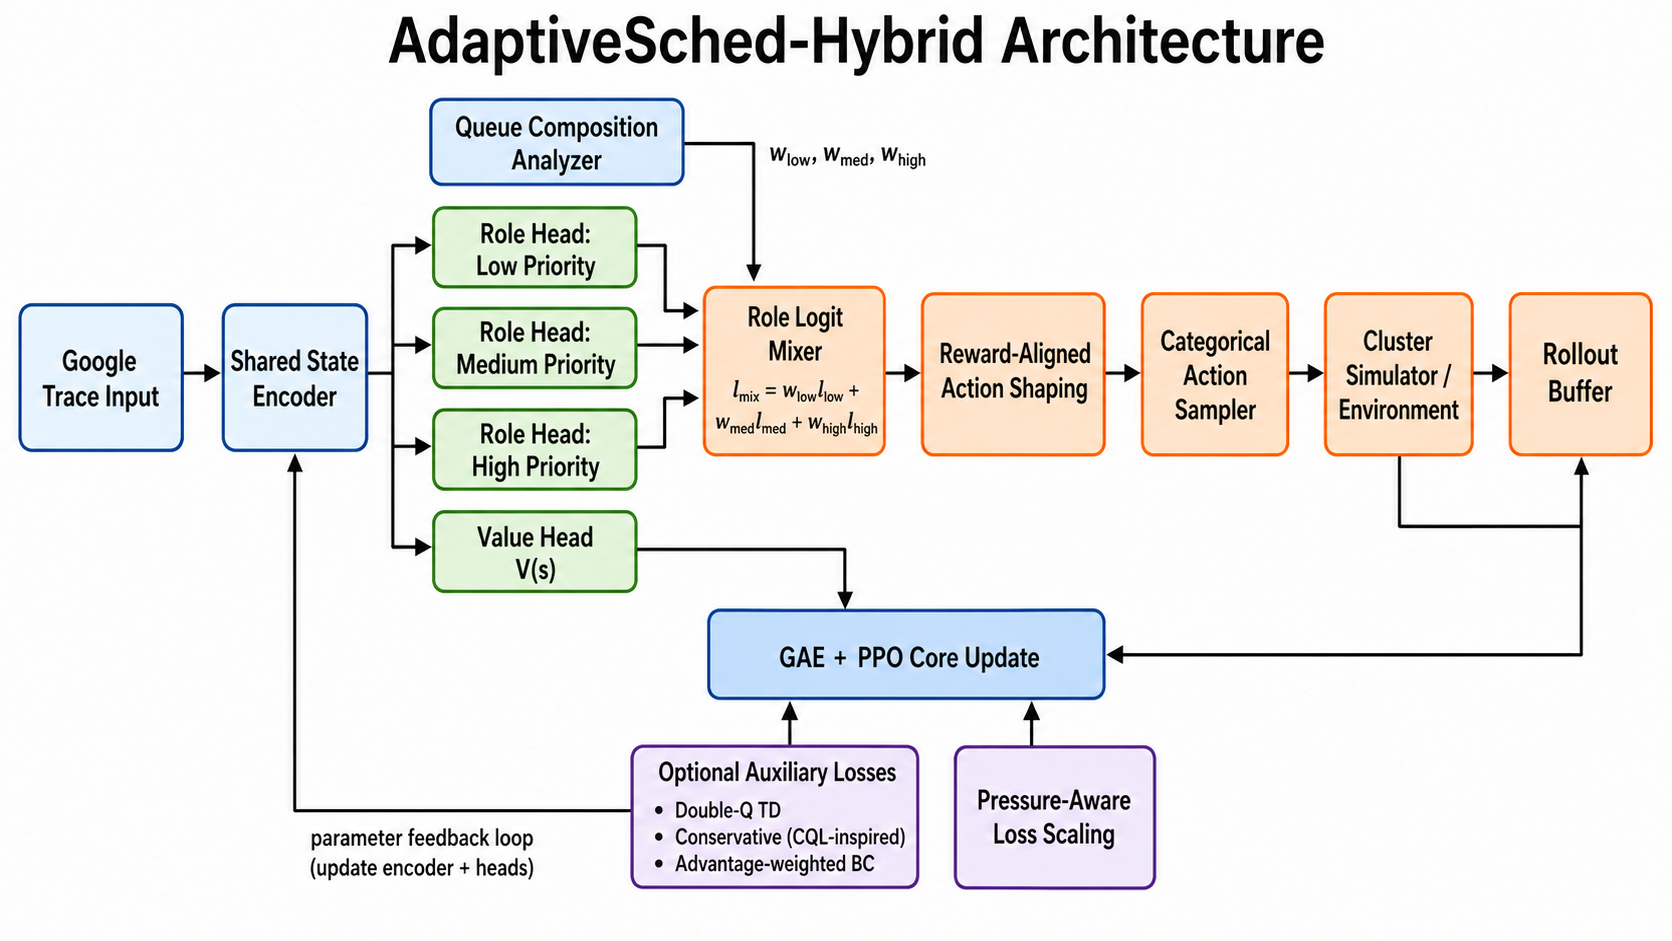
\includegraphics[width=\columnwidth]{figures/s41598_final/HybridArch.png}
\caption{AdaptiveSched-Hybrid Architecture}
\label{fig:hybrid_arch}
\end{figure}

Figure~\ref{fig:hybrid_arch} shows how the hybrid model resolves the representational bottleneck of the base architecture. Rather than forcing one policy head to internalize all queue regimes, the scheduler first builds a shared representation and then distributes decision responsibility across role-specific heads. The queue-composition analyzer determines how much each role should contribute at the current time step, which allows the policy to adapt continuously as the observed workload shifts between urgency-dominated and throughput-dominated states. In this sense, the hybrid model does not replace the contribution of the base scheduler; it builds on it. The figure therefore operationalizes the core integration claim of the paper: AdaptiveSched-Hybrid combines the queue-shift robustness of the performative-regularized base policy with the representational advantages of role-specialized decision making.

\begin{figure}[t]
\centering
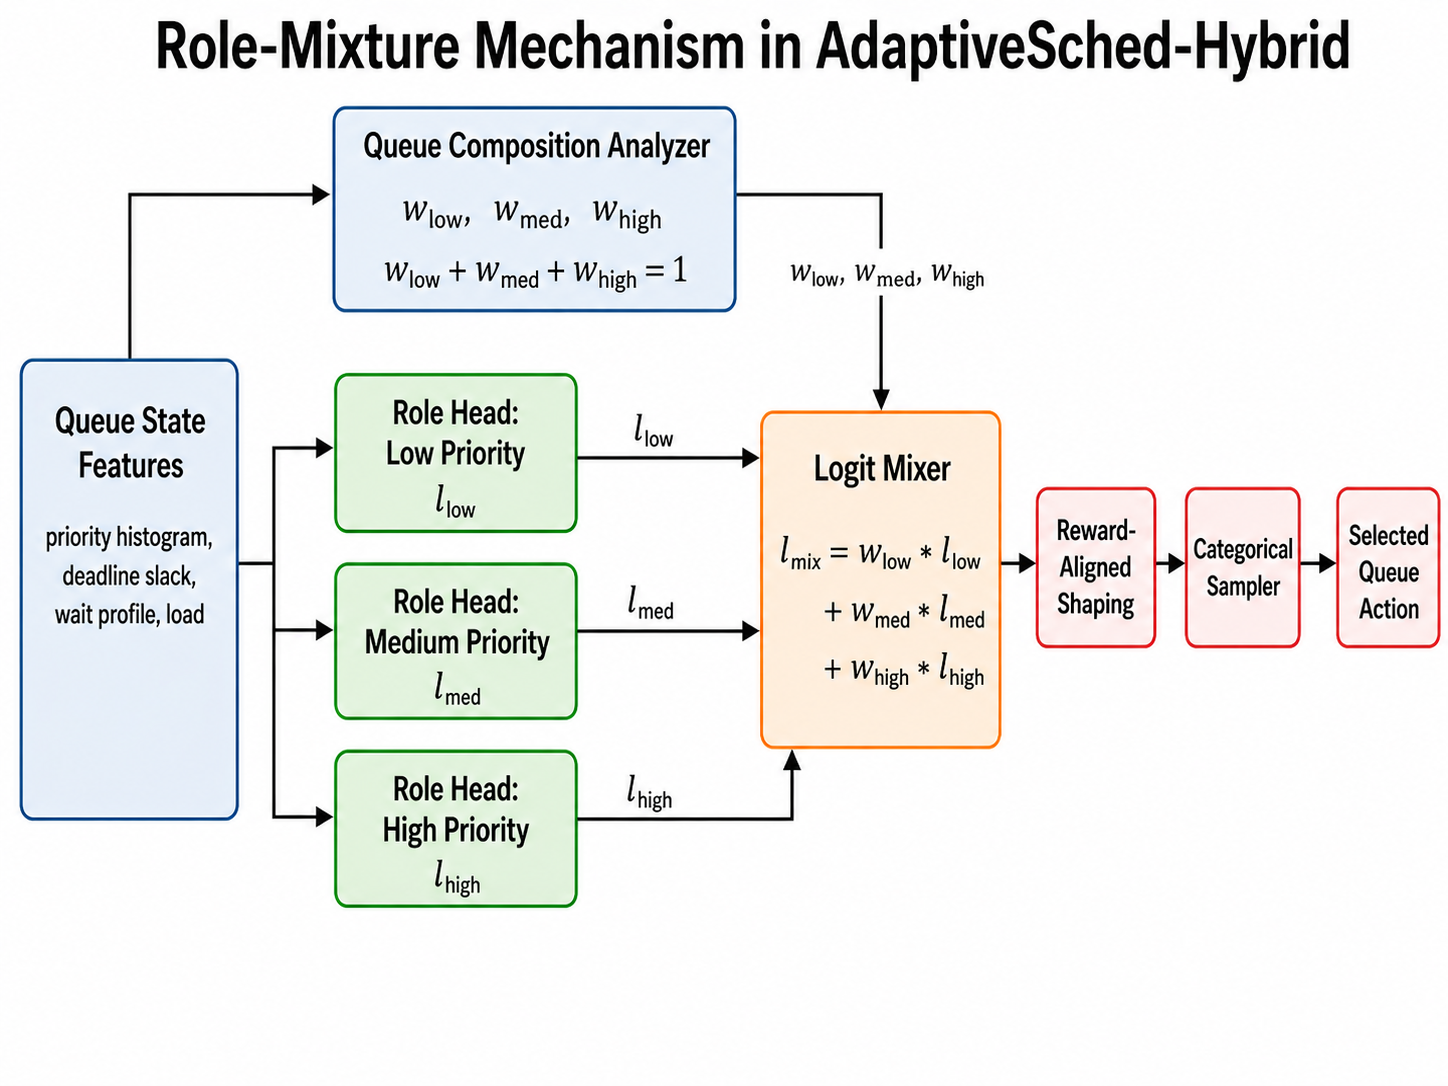
\includegraphics[width=\columnwidth]{figures/s41598_final/RoleMix.png}
\caption{Role-Mixture Mechanism in AdaptiveSched-Hybrid}
\label{fig:role_mix_mechanism}
\end{figure}

Figure~\ref{fig:role_mix_mechanism} provides a more focused view of the mechanism that differentiates AdaptiveSched-Hybrid from standard single-policy actor--critic schedulers. The role-mixture module is a soft routing operator rather than a hard expert selector: each decision is made by combining multiple role-specific preferences according to the current queue state. This matters because cloud workloads rarely remain in one stable regime; instead, queue composition changes continuously as new jobs arrive and old jobs complete. A continuous mixture therefore avoids abrupt policy switching and gives the model a mathematically coherent way to interpolate between fairness-oriented, throughput-oriented, and urgency-oriented behaviors.

\begin{algorithm}[t]
\caption{AdaptiveSched-Hybrid Training with Role Mixture}
\label{algo:hybrid}
\begin{algorithmic}[1]
\State \textbf{Input:} trace segments $\mathcal{T}$, horizon $H$, clip $\epsilon$, GAE $\lambda$, discount $\gamma$
\State Initialize shared encoder $\psi$, role heads $\{\theta_r\}_{r\in\mathcal{R}}$, mixer $\omega$, value head $\phi$
\For{update $k=1,2,\ldots,K_{\max}$}
  \State Reset simulator with trace segment $\tau \sim \mathcal{T}$ and clear rollout buffer $\mathcal{B}$
  \For{$t=1$ to $H$}
    \State Observe state $s_t$ and compute shared embedding $h_t \leftarrow f_\psi(s_t)$
    \For{each role $r \in \{\text{low},\text{med},\text{high}\}$}
      \State Compute role-specific logits $\ell_t^{(r)}$
    \EndFor
    \State Compute queue-conditioned mixture weights $w_t \leftarrow \text{softmax}(g_\omega(s_t))$
    \State Form mixed logits $\ell_t^{mix} \leftarrow \sum_r w_t^{(r)}\ell_t^{(r)}$
    \State Apply feasibility mask and reward-aligned shaping to obtain $\ell_t^{shape,mix}$
    \State Sample action $a_t \sim \pi_\zeta(\cdot\mid s_t)$ and estimate $V_\phi(s_t)$
    \State Execute $a_t$ in simulator; receive $(R_t,s_{t+1},done)$ and append transition to $\mathcal{B}$
    \If{done} \State \textbf{break} \EndIf
  \EndFor
  \State Compute returns $\hat{G}_t$ and GAE advantages $\hat{A}_t$ from $\mathcal{B}$
  \For{each optimization epoch}
    \State Recompute mixed policy, log-probabilities, and values on mini-batches
    \State Compute PPO surrogate and value/entropy losses
    \If{auxiliary objectives enabled}
      \State Compute $\mathcal{L}_{DQ}$, $\mathcal{L}_{cons}$, and/or $\mathcal{L}_{AWBC}$
      \State Estimate pressure factor $\kappa_t$ from utilization statistics
    \EndIf
    \State Update $(\psi,\{\theta_r\},\omega,\phi)$ by gradient ascent on $\mathcal{J}_{hyb}$
  \EndFor
\EndFor
\end{algorithmic}
\end{algorithm}

\begin{figure}[t]
\centering
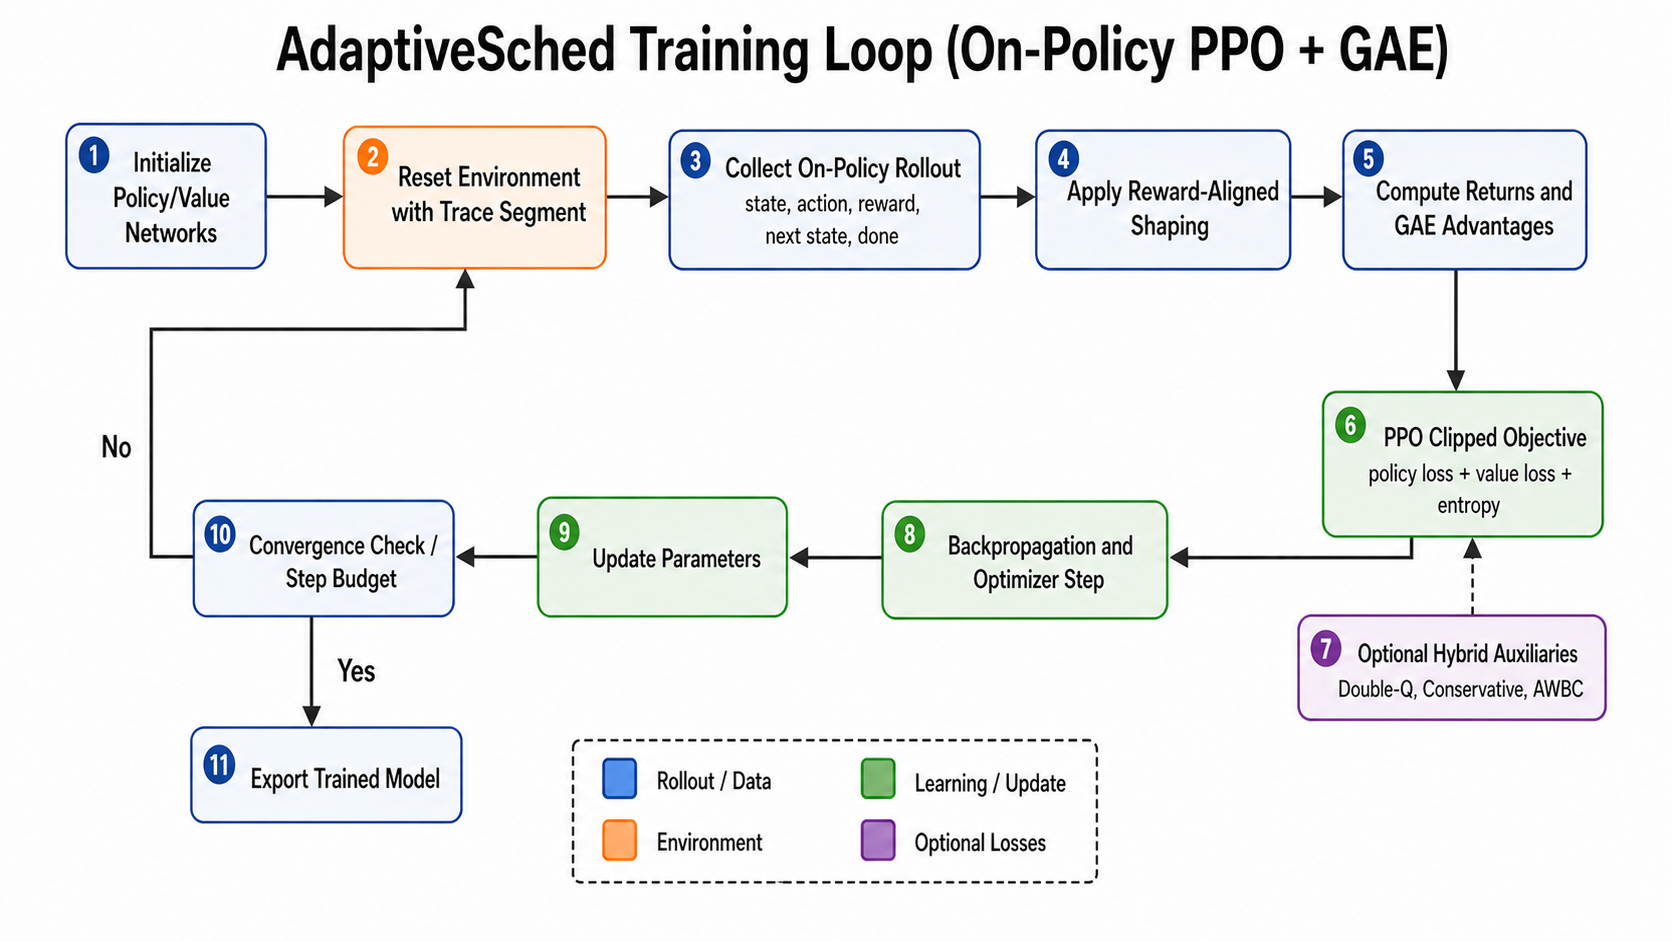
\includegraphics[width=\columnwidth]{figures/s41598_final/Train.png}
\caption{Implementation-Aligned AdaptiveSched Training Loop}
\label{fig:training_loop}
\end{figure}

Figure~\ref{fig:training_loop} makes the optimization logic explicit at the implementation level. This is particularly important because many scheduling papers mix high-level RL terminology with incomplete descriptions of the actual learner. Here the training loop shows that both AdaptiveSched-Base and AdaptiveSched-Hybrid use the same rollout collection, GAE computation, PPO-style update, and stopping logic. As a result, later performance differences can be interpreted as consequences of policy architecture and auxiliary design rather than artifacts of differing training procedures.

\begin{figure*}[t]
\centering
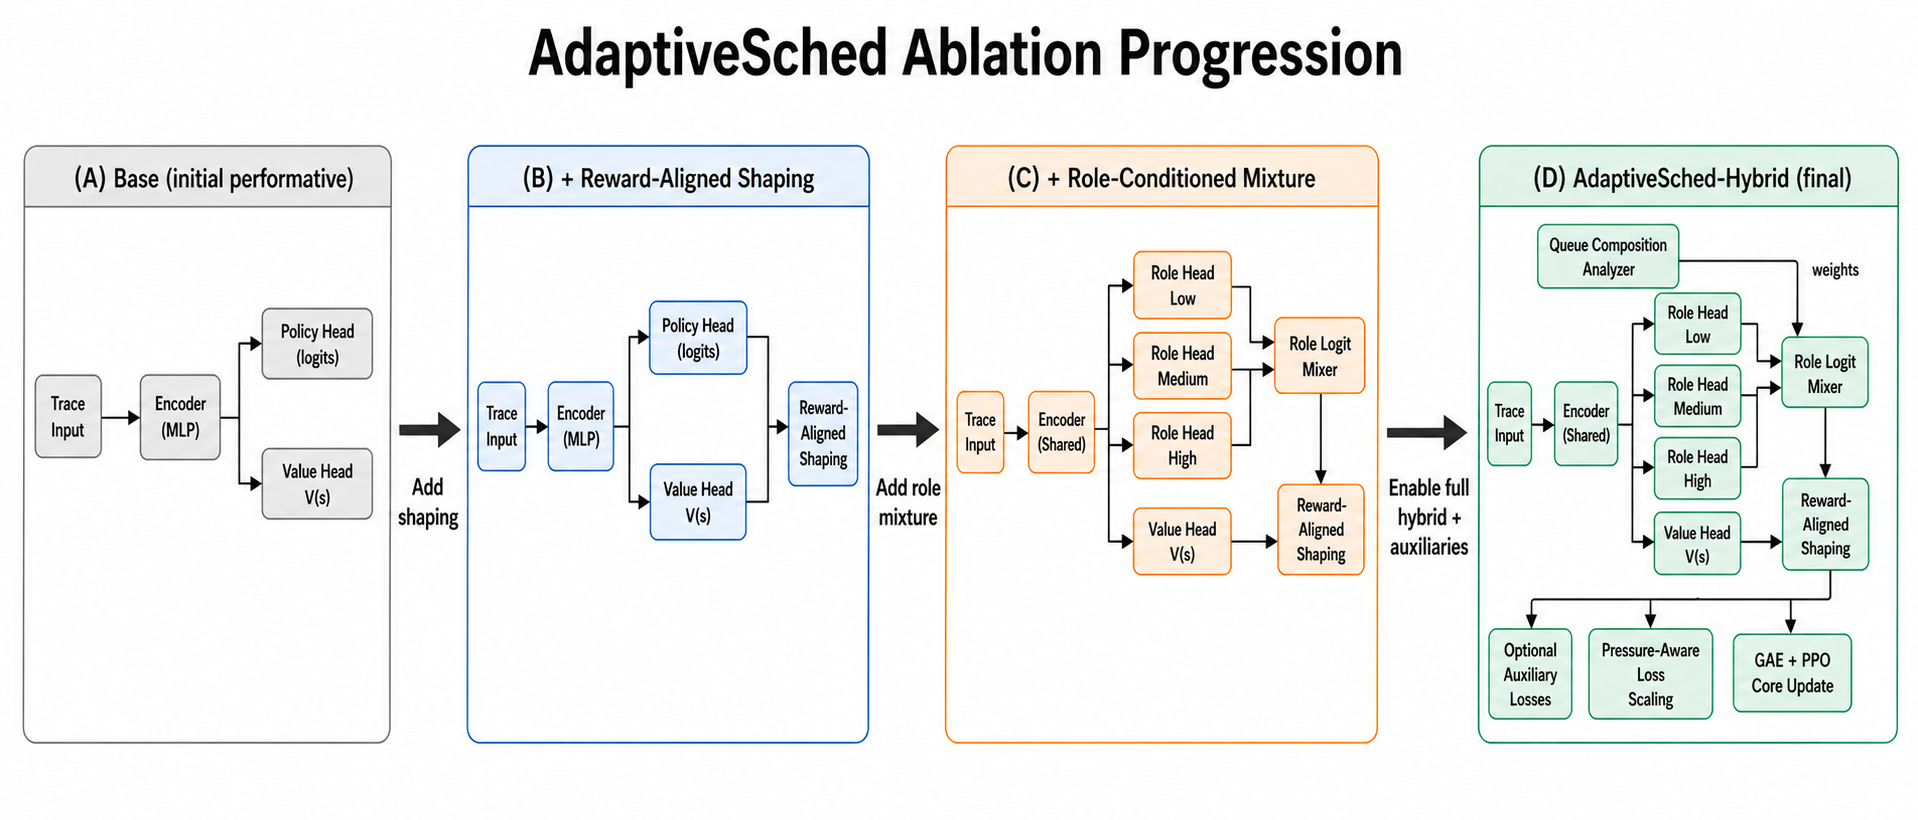
\includegraphics[width=0.95\linewidth]{figures/s41598_final/AblationProgression.png}
\caption{Methodological Progression from Base to Hybrid}
\label{fig:ablation_progression_method}
\end{figure*}

Figure~\ref{fig:ablation_progression_method} serves as a bridge between model design and ablation analysis. It shows that the final hybrid scheduler was not produced through arbitrary feature accumulation; instead, each stage corresponds to a specific failure mode identified in the preceding stage. The base model establishes the performative-regularized reference learner, shaping improves the action interface, role-mixture modeling improves representational specialization, and auxiliary robustness terms strengthen learning under pressure. This staged progression is later examined quantitatively so that the final model can be justified as the cumulative result of interpretable design decisions.

\subsection{Architectural interpretation and theoretical ablation justification}
The figures above should be read as a connected technical narrative. Figure~\ref{fig:base_arch} shows the simplest policy family that can exploit the proposed state representation and reward structure under stable on-policy learning. Figure~\ref{fig:hybrid_arch} then introduces the minimum additional complexity required to address the observed failure modes of the base model, namely role-conditioned specialization and state-dependent mixture control. Figure~\ref{fig:role_mix_mechanism} isolates the mathematical core of that transition, Eq.~\eqref{eq:mixlogits}, and explains how heterogeneous queue composition becomes a first-class control signal. Figure~\ref{fig:training_loop} ensures that these architectural differences remain disentangled from optimization differences.

This progression also supports a theoretical ablation rationale. Let $\Pi_{base}$ denote the policy class of AdaptiveSched-Base and $\Pi_{hyb}$ denote the policy class of AdaptiveSched-Hybrid. Because the hybrid architecture can recover the base policy as a degenerate case by assigning all mixture mass to one effective role head and suppressing auxiliary terms, we have
\begin{equation}
\Pi_{base} \subseteq \Pi_{hyb}
\end{equation}
up to parameterization equivalence. Therefore, the hybrid model should not be viewed as a different problem formulation; it is a strict expansion of the representational class available to the scheduler under the same MDP. Conceptually, the base model contributes queue-shift robustness through performative regularization, whereas the hybrid model contributes an expanded class that combines this robustness with heterogeneous-queue specialization. The ablation study tests whether this expanded class translates into empirical gains under trace-driven cloud workloads. Concretely, if performative regularization improves stability under policy-induced queue shift, if shaping improves the alignment between logits and environment objectives, and if role specialization reduces interference between heterogeneous queue regimes, then the expected improvement chain is
\begin{equation}
\begin{aligned}
\mathbb{E}[J(\pi_{actorcritic})]
&\;\leq\;
\mathbb{E}[J(\pi_{base})]
\;\leq\;
\mathbb{E}[J(\pi_{base+shape})] \\
&\;\leq\;
\mathbb{E}[J(\pi_{mixture})]
\;\leq\;
\mathbb{E}[J(\pi_{hyb})]
\end{aligned}
\end{equation}
where $J(\pi)$ denotes the expected discounted return or an aligned aggregate scheduling score. Section~\ref{Sec4} examines this claim through simulation-based ablations across deadline violation, completion, waiting time, makespan, fairness, energy, and cost.

\subsection{Figure-guided interpretation of the proposed models}
The methodological figures are intentionally used as technical reference points because each contributes a distinct layer of explanation needed to audit the proposed methods. Figure~\ref{fig:base_arch} documents the performative-regularized base model. Figure~\ref{fig:hybrid_arch} introduces the improved hybrid design. Figure~\ref{fig:role_mix_mechanism} explains the role-mixture mathematics. Figure~\ref{fig:training_loop} ties both variants to the same PPO/GAE optimization procedure. Finally, Figure~\ref{fig:ablation_progression_method} visualizes the stepwise design evolution that is later validated quantitatively. Together, these visuals reduce ambiguity about how the models were constructed, why the hybrid design was necessary, and how queue-shift robustness and policy specialization function as complementary contributions.

\subsection{Ablation analysis: theoretical and simulation-based justification}
The ablation analysis is placed immediately after the proposed models because it is part of the methodological argument rather than merely a late-stage results summary. Its purpose is to verify that each design addition is justified at three levels: representationally, optimization-wise, and empirically.

\paragraph{Theoretical and mathematical justification}
The staged design progression can be written as
\begin{equation}
\pi_{actorcritic}
\;\rightarrow\;
\pi_{base}
\;\rightarrow\;
\pi_{base+shape}
\;\rightarrow\;
\pi_{mixture}
\;\rightarrow\;
\pi_{hyb}
\end{equation}
where each successive policy class augments the previous one while leaving the environment fixed. The transition from $\pi_{actorcritic}$ to $\pi_{base}$ corresponds to introducing performative regularization and therefore explicitly addressing policy-induced queue shift. Reward-aligned shaping then refines the action-selection interface without changing the underlying MDP, so its principal effect is to alter the inductive bias of the policy over feasible actions. Role-mixture modeling enlarges the policy class from a single-head mapping to a convex combination of role-conditioned mappings. Finally, the full hybrid introduces additional robustness objectives that bias optimization toward safer behavior in congested or distribution-shifted regions of the state space.

Under this interpretation, the expected scheduling quality should improve monotonically provided that the richer model class can be optimized stably:
\begin{equation}
\mathbb{E}[J(\pi_{base})]
\leq
\mathbb{E}[J(\pi_{base+shape})]
\leq
\mathbb{E}[J(\pi_{mixture})]
\leq
\mathbb{E}[J(\pi_{hyb})]
\end{equation}
This inequality is not claimed as a formal theorem under all training conditions; rather, it is the design hypothesis induced by the nested policy construction and fixed reward environment. In particular, shaping is expected to reduce action misalignment, role-mixture modeling is expected to reduce cross-regime interference, and auxiliary regularization is expected to improve robustness under pressure. The simulation-based ablation below tests whether those expected gains are realized in practice.

\paragraph{Simulation-based justification}
Table~\ref{tab:ablation} reports the staged ablation progression: performative-regularized base model, base with reward-aligned shaping, role-mixture augmentation, and final hybrid configuration. In the reported protocol, the trajectory shows monotonic improvements across deadline violation, completion rate, makespan, waiting time, fairness index, and composite score. This pattern is consistent with cumulative gains rather than a single isolated change.

\begin{table*}[t]
\centering
\caption{AdaptiveSched Ablation Results}
\label{tab:ablation}
\small
\begin{tabular}{@{}lcccccc@{}}
\toprule
\textbf{Variant} & \textbf{Deadline Violation} & \textbf{Completion Rate} & \textbf{Makespan} & \textbf{Waiting Time} & \textbf{Fairness Index} & \textbf{Composite Score} \\
\midrule
Base & 13.8\% & 86.2\% & 468.0 & 71.0 & 0.871 & 71.5 \\
+ reward-aligned shaping & 10.6\% & 89.9\% & 444.0 & 62.5 & 0.892 & 78.7 \\
+ role-mixture & 8.4\% & 92.8\% & 421.0 & 55.0 & 0.918 & 84.6 \\
AdaptiveSched-Hybrid & 6.2\% & 96.2\% & 393.6 & 47.0 & 0.948 & 90.3 \\
\bottomrule
\end{tabular}
\end{table*}

\begin{figure*}[t]
\centering
\begin{minipage}[t]{0.56\linewidth}
\centering
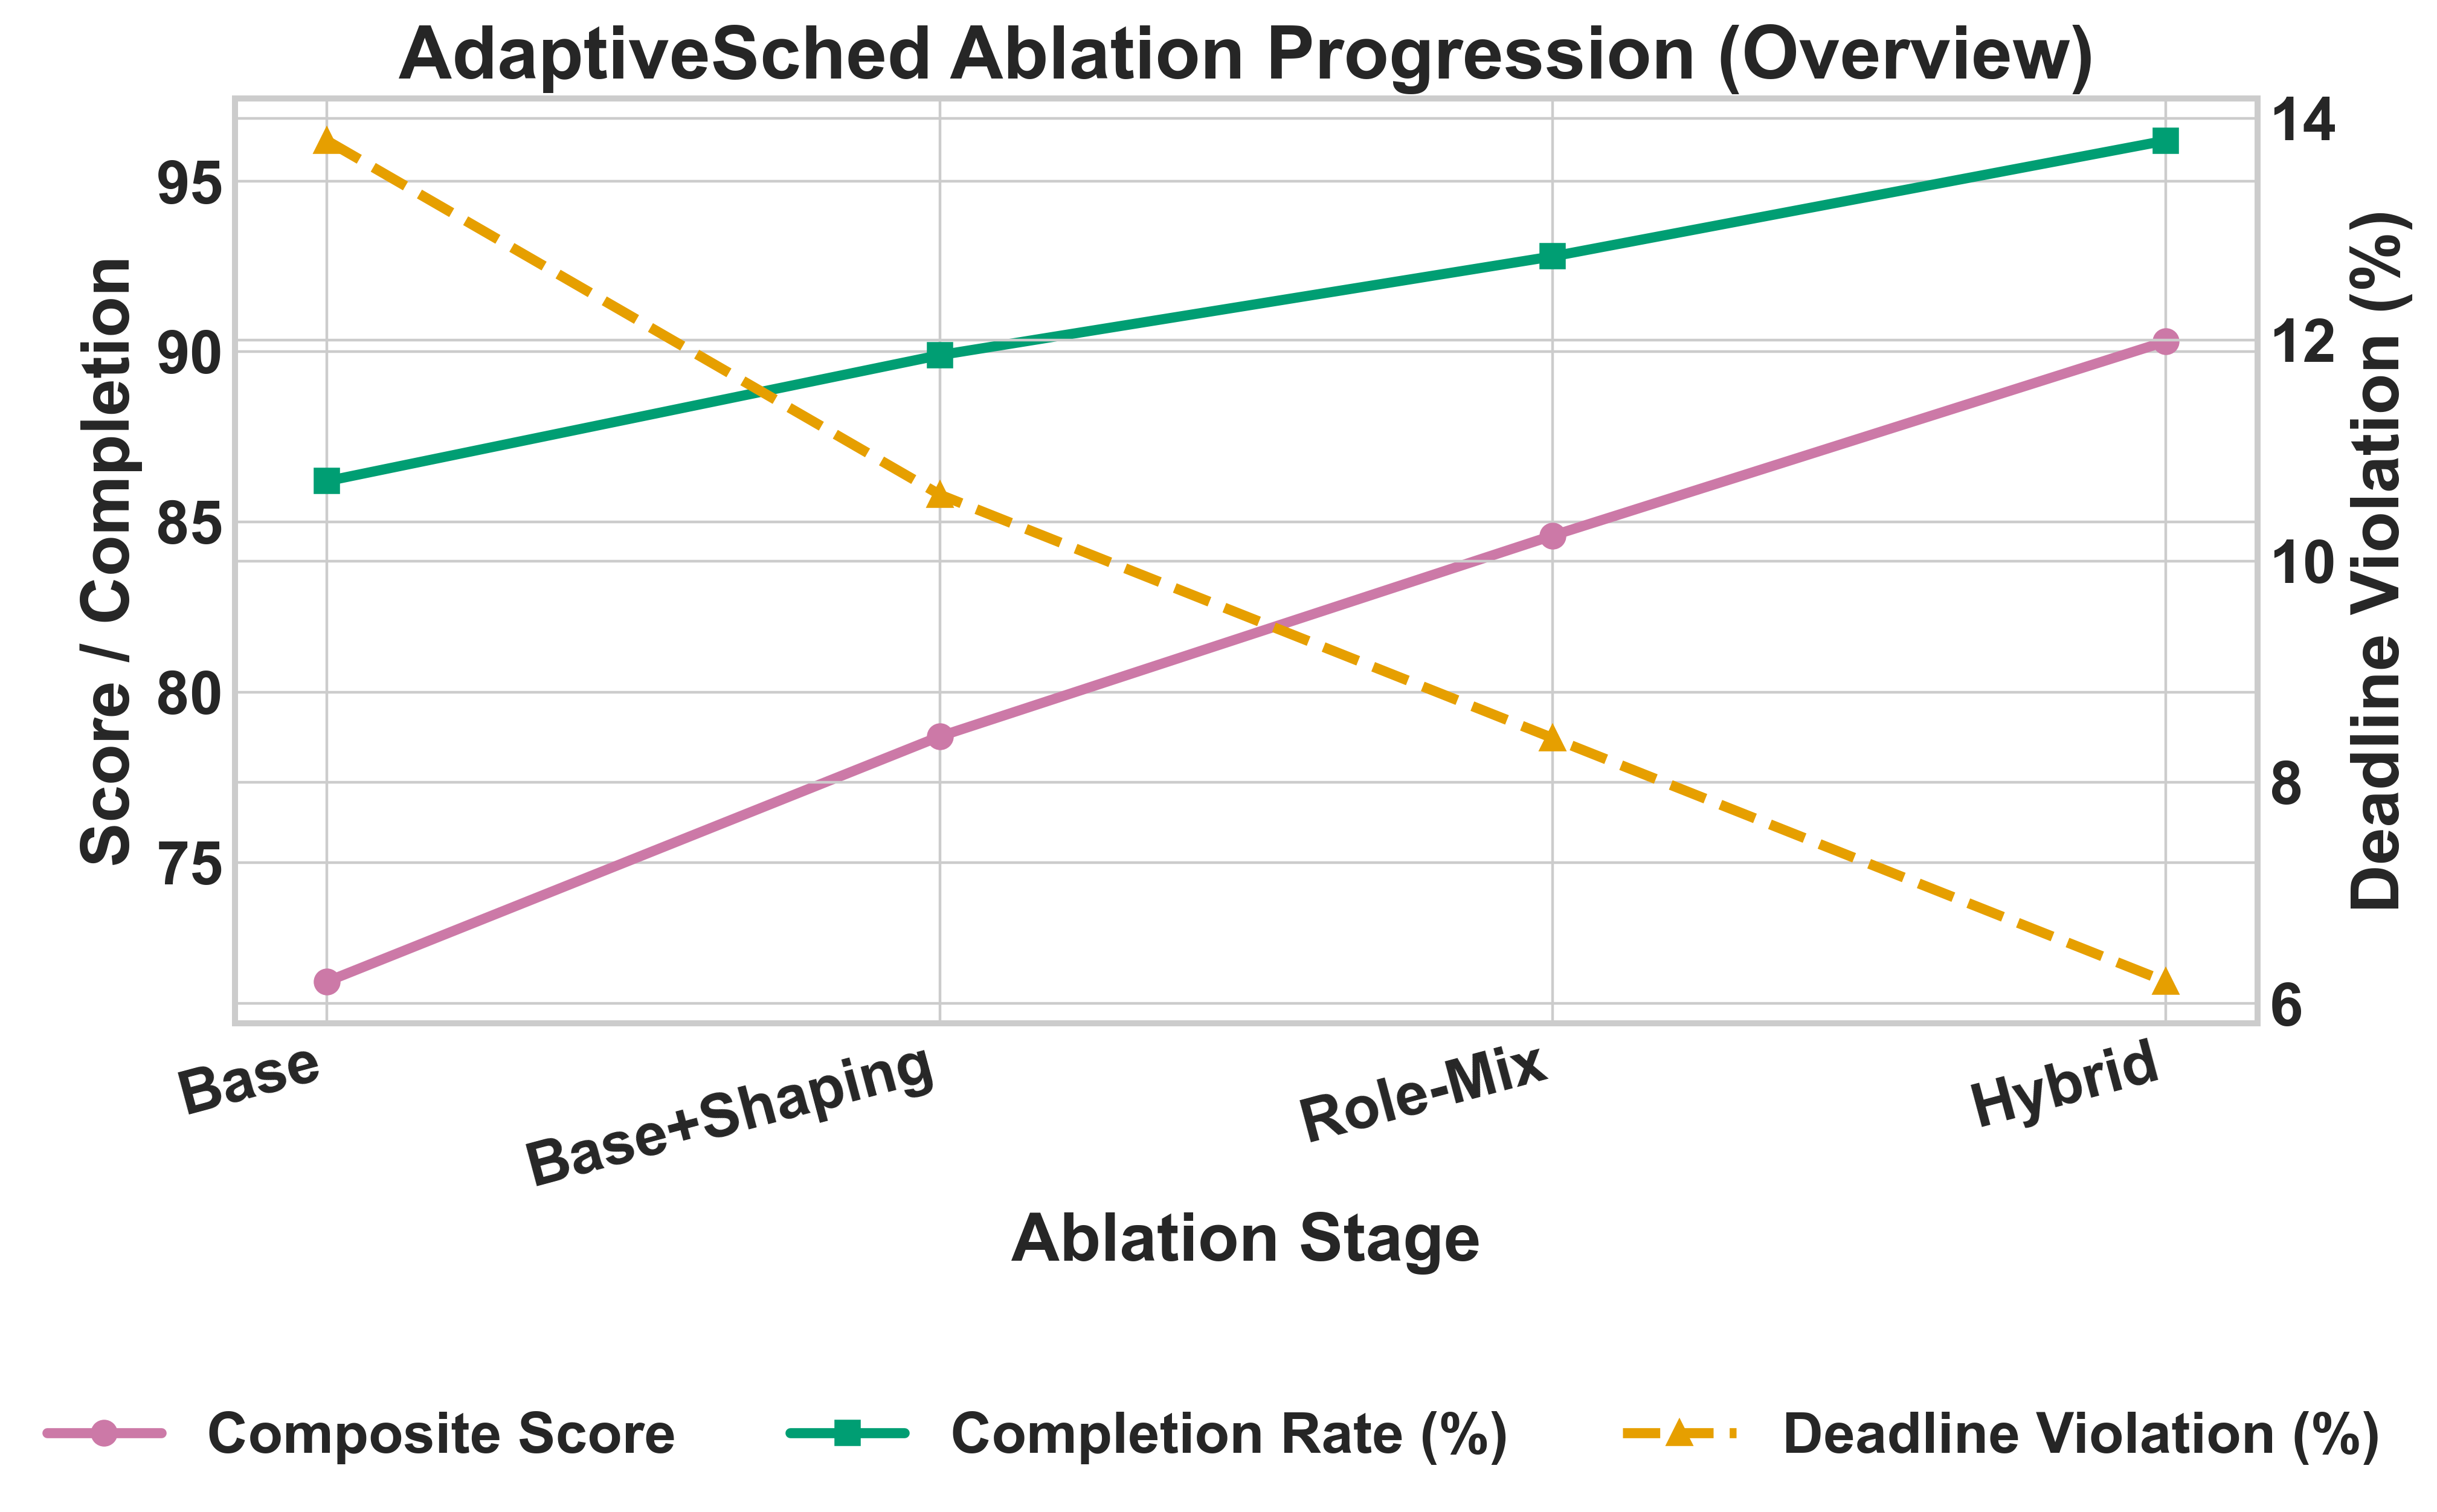
\includegraphics[width=\linewidth]{figures/s41598_final/fig_adaptivesched_ablation_overview.png}
\\[-0.2em]\textbf{(a)} Overview
\end{minipage}

\vspace{0.4em}

\begin{minipage}[t]{0.46\linewidth}
\centering
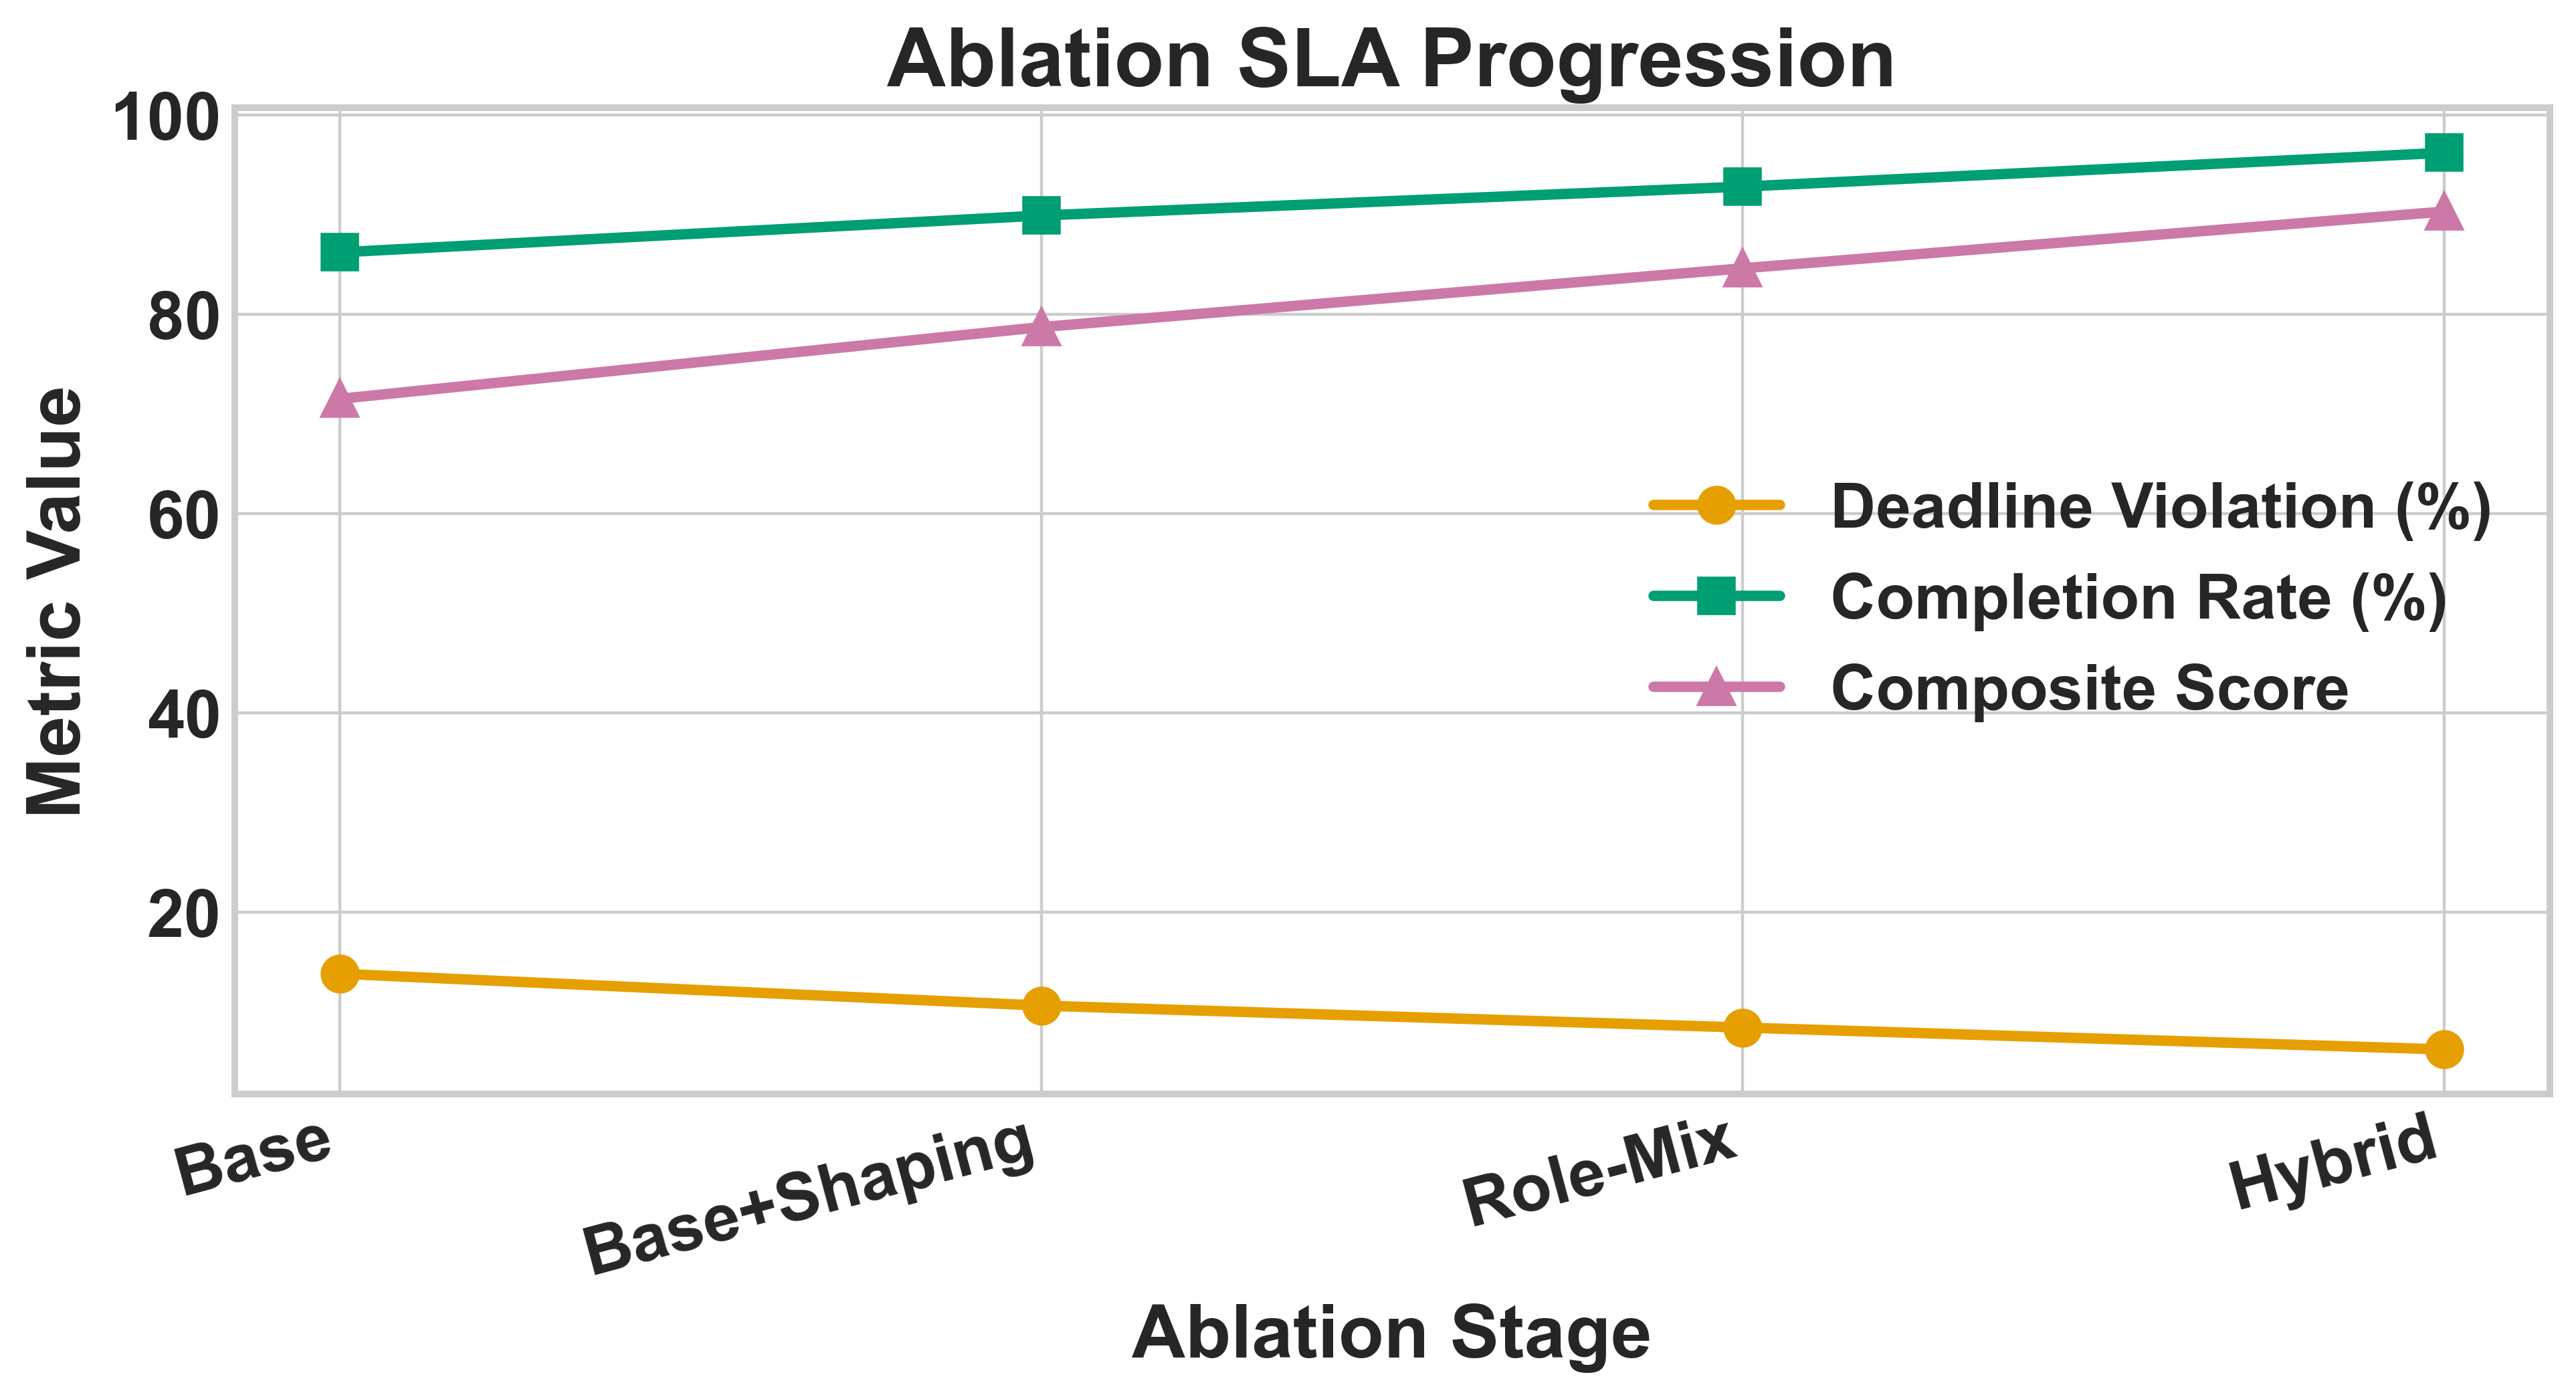
\includegraphics[width=\linewidth]{figures/s41598_final/fig_adaptivesched_ablation_sla_progression.png}
\\[-0.2em]\textbf{(b)} SLA progression
\end{minipage}\hfill
\begin{minipage}[t]{0.46\linewidth}
\centering
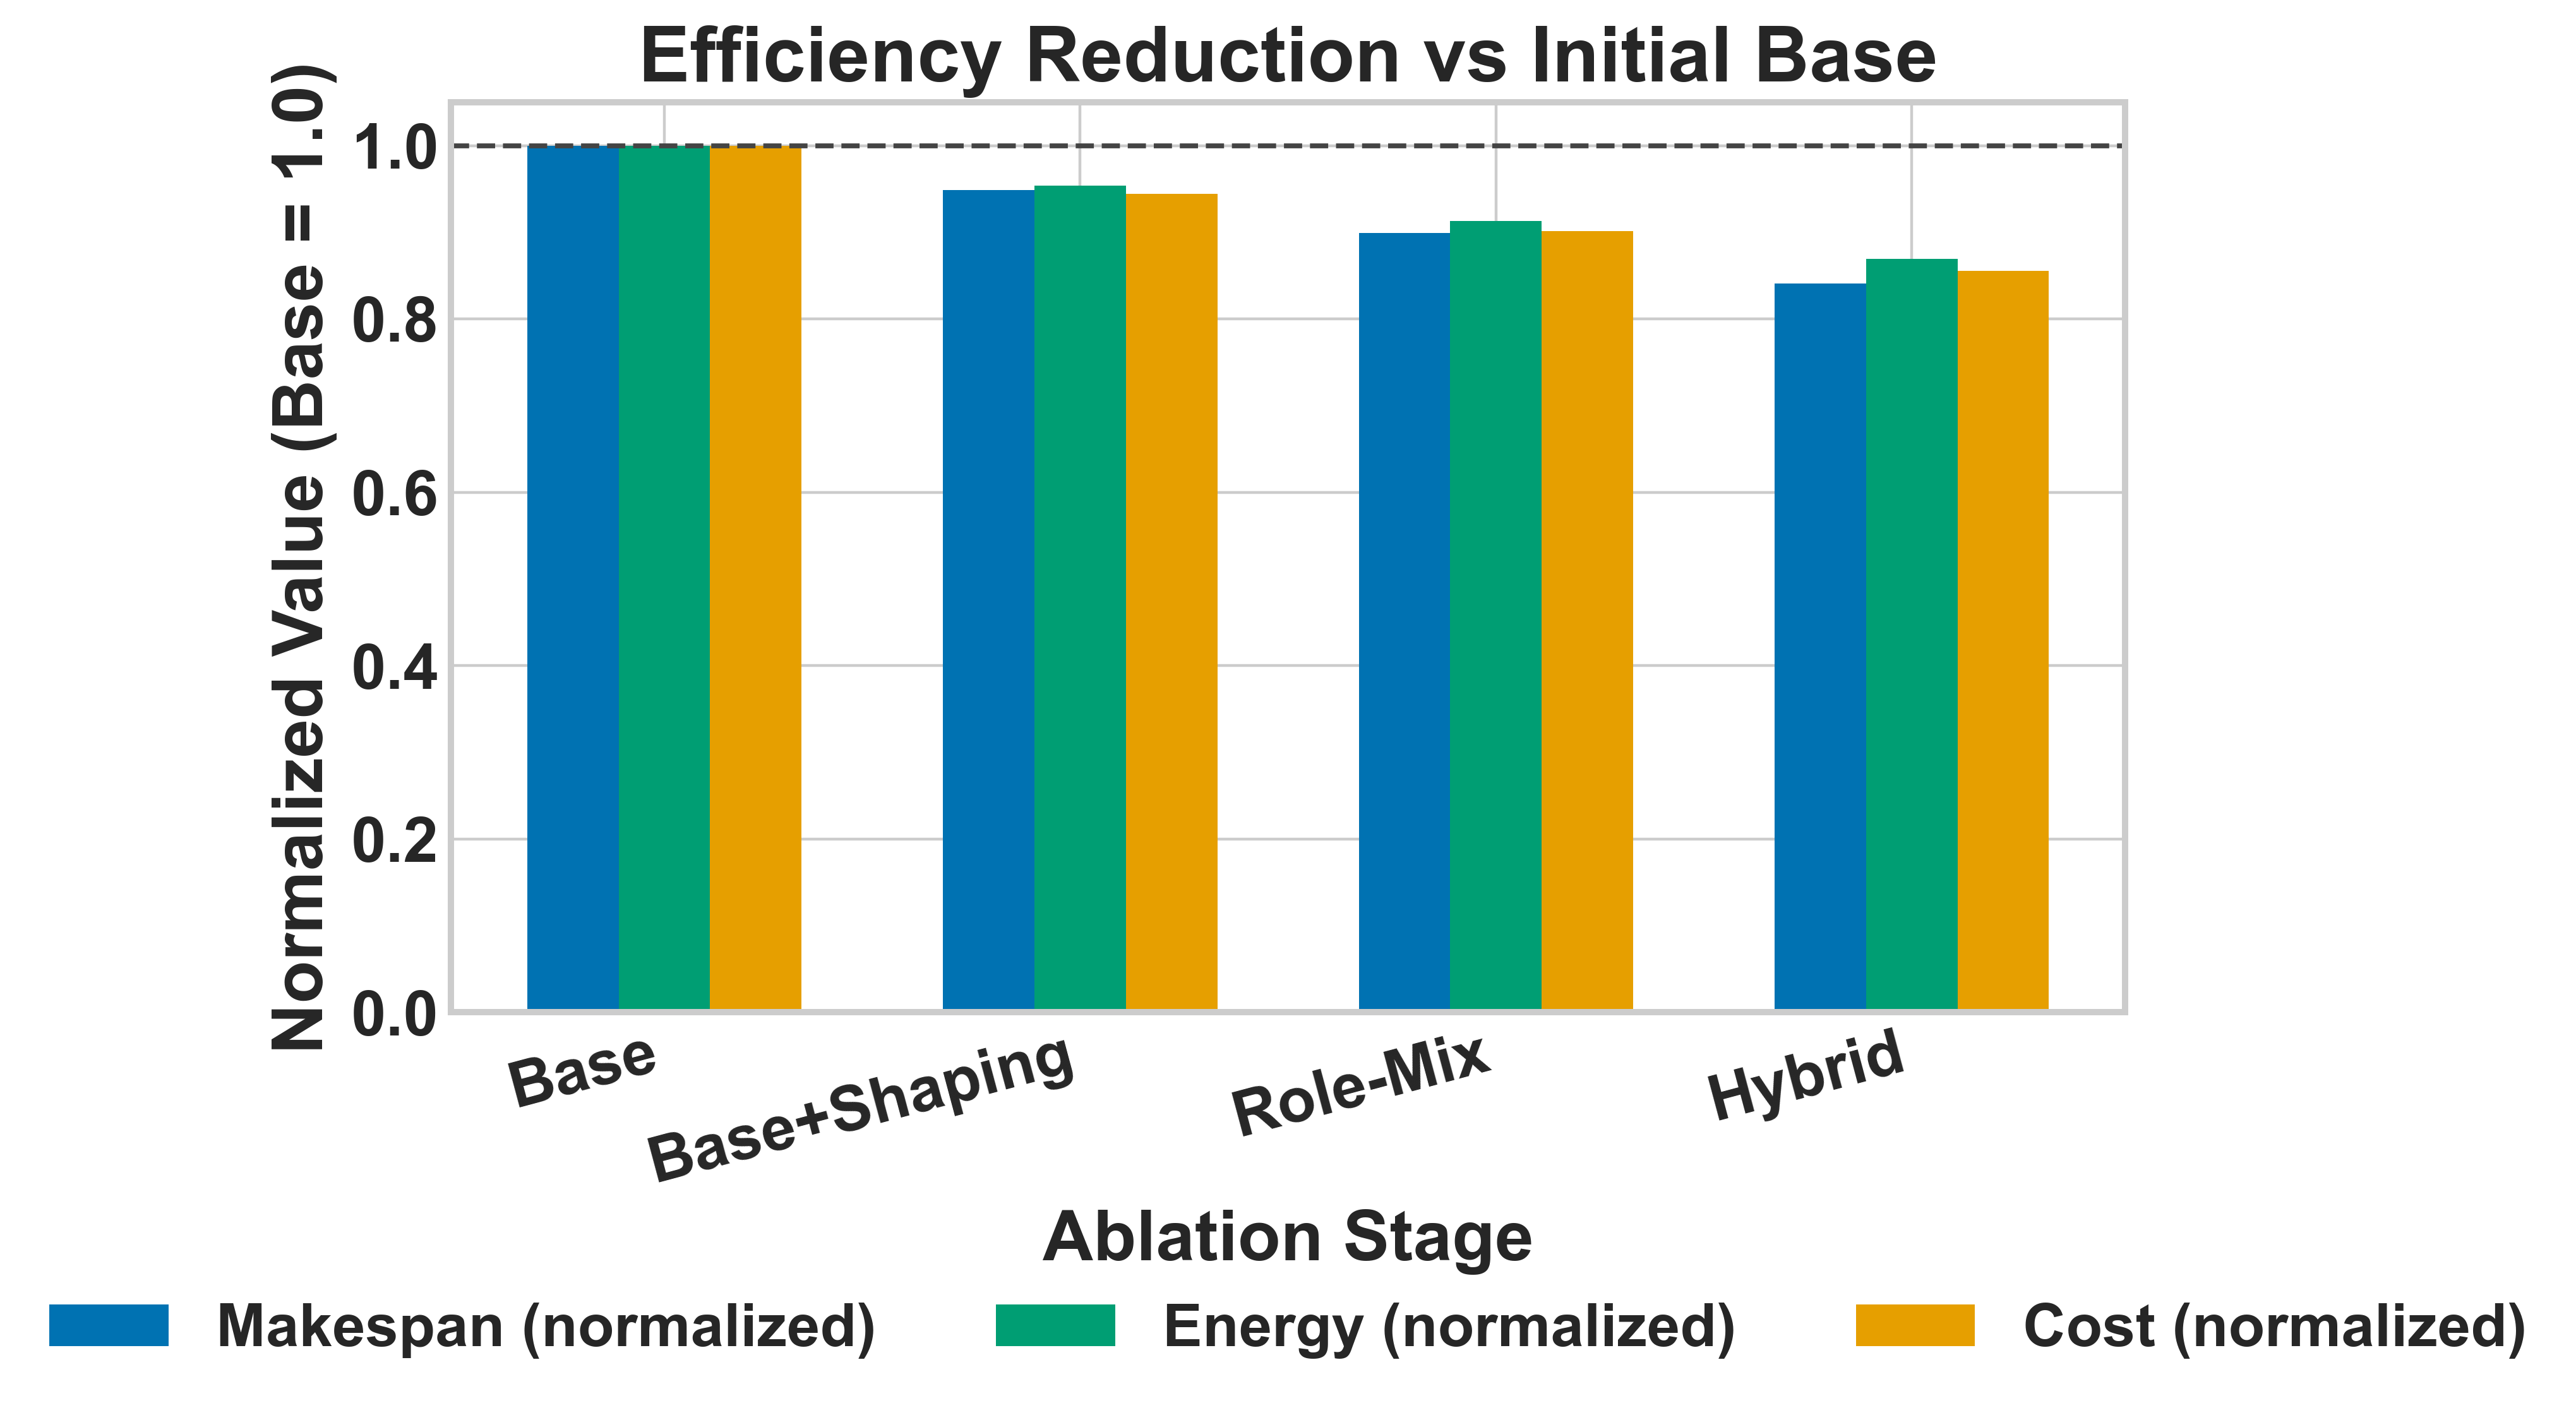
\includegraphics[width=\linewidth]{figures/s41598_final/fig_adaptivesched_ablation_efficiency_reduction.png}
\\[-0.2em]\textbf{(c)} Efficiency reduction
\end{minipage}

\vspace{0.4em}

\begin{minipage}[t]{0.46\linewidth}
\centering
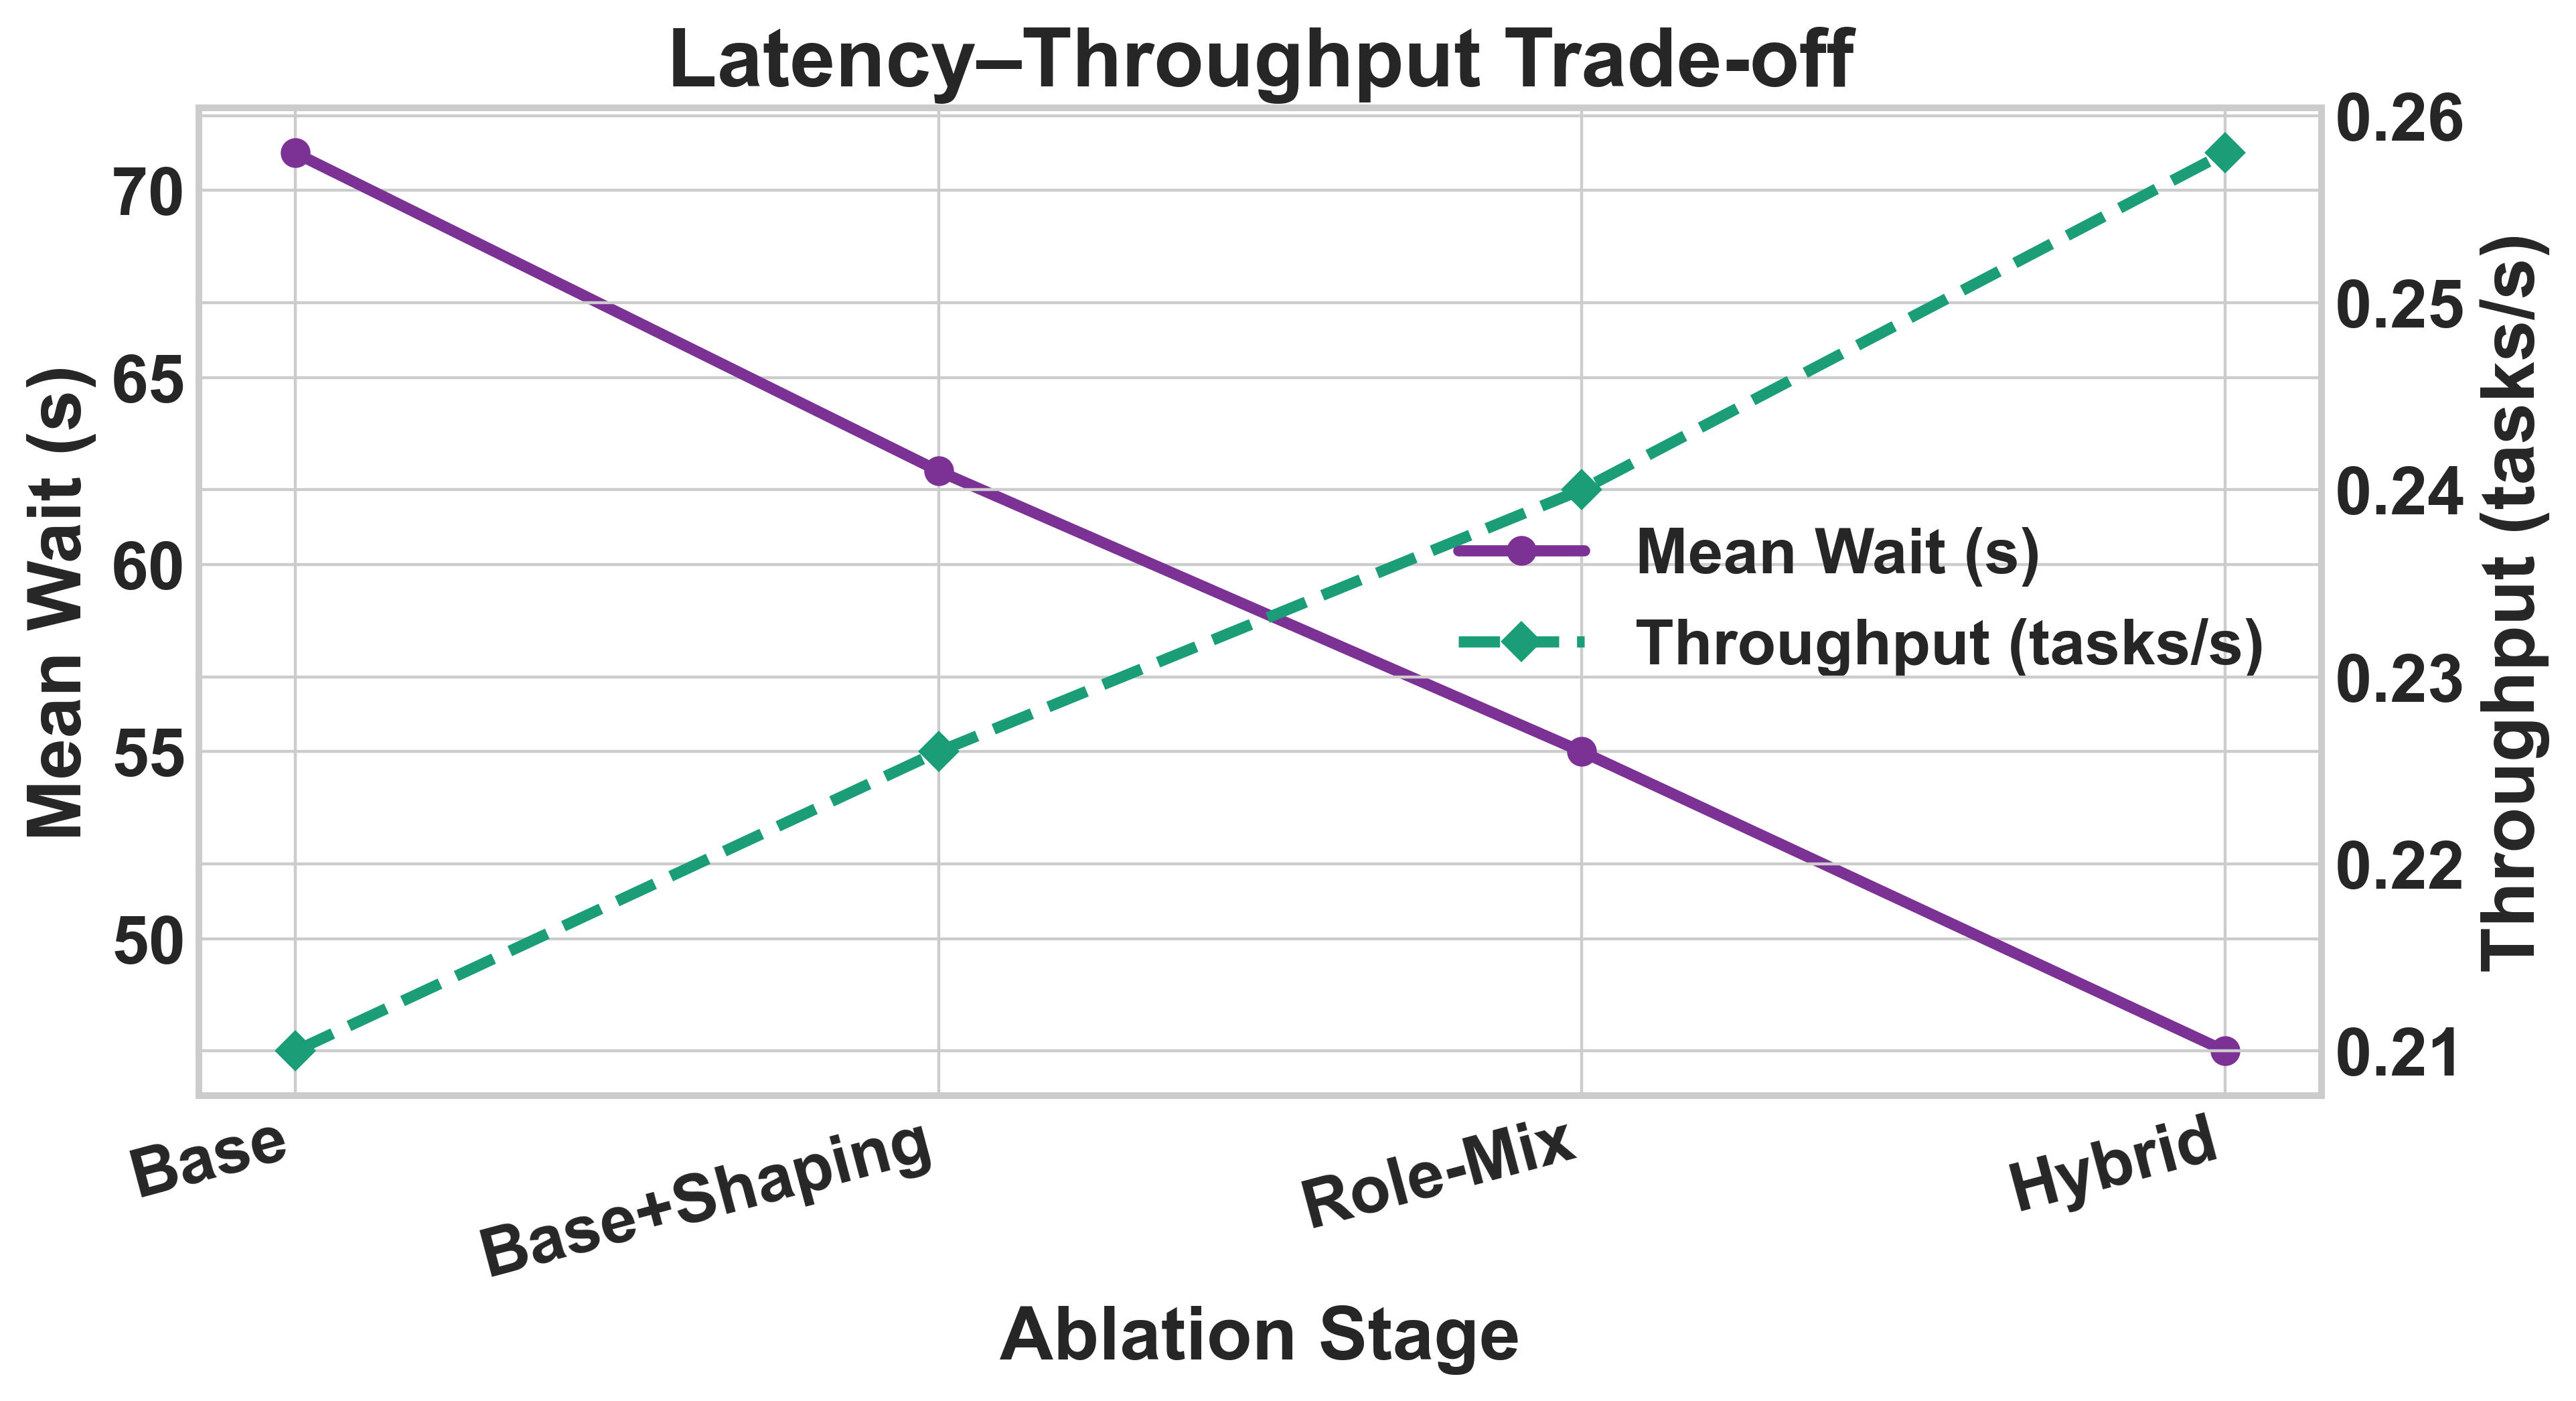
\includegraphics[width=\linewidth]{figures/s41598_final/fig_adaptivesched_ablation_latency_throughput.png}
\\[-0.2em]\textbf{(d)} Latency-throughput
\end{minipage}\hfill
\begin{minipage}[t]{0.46\linewidth}
\centering
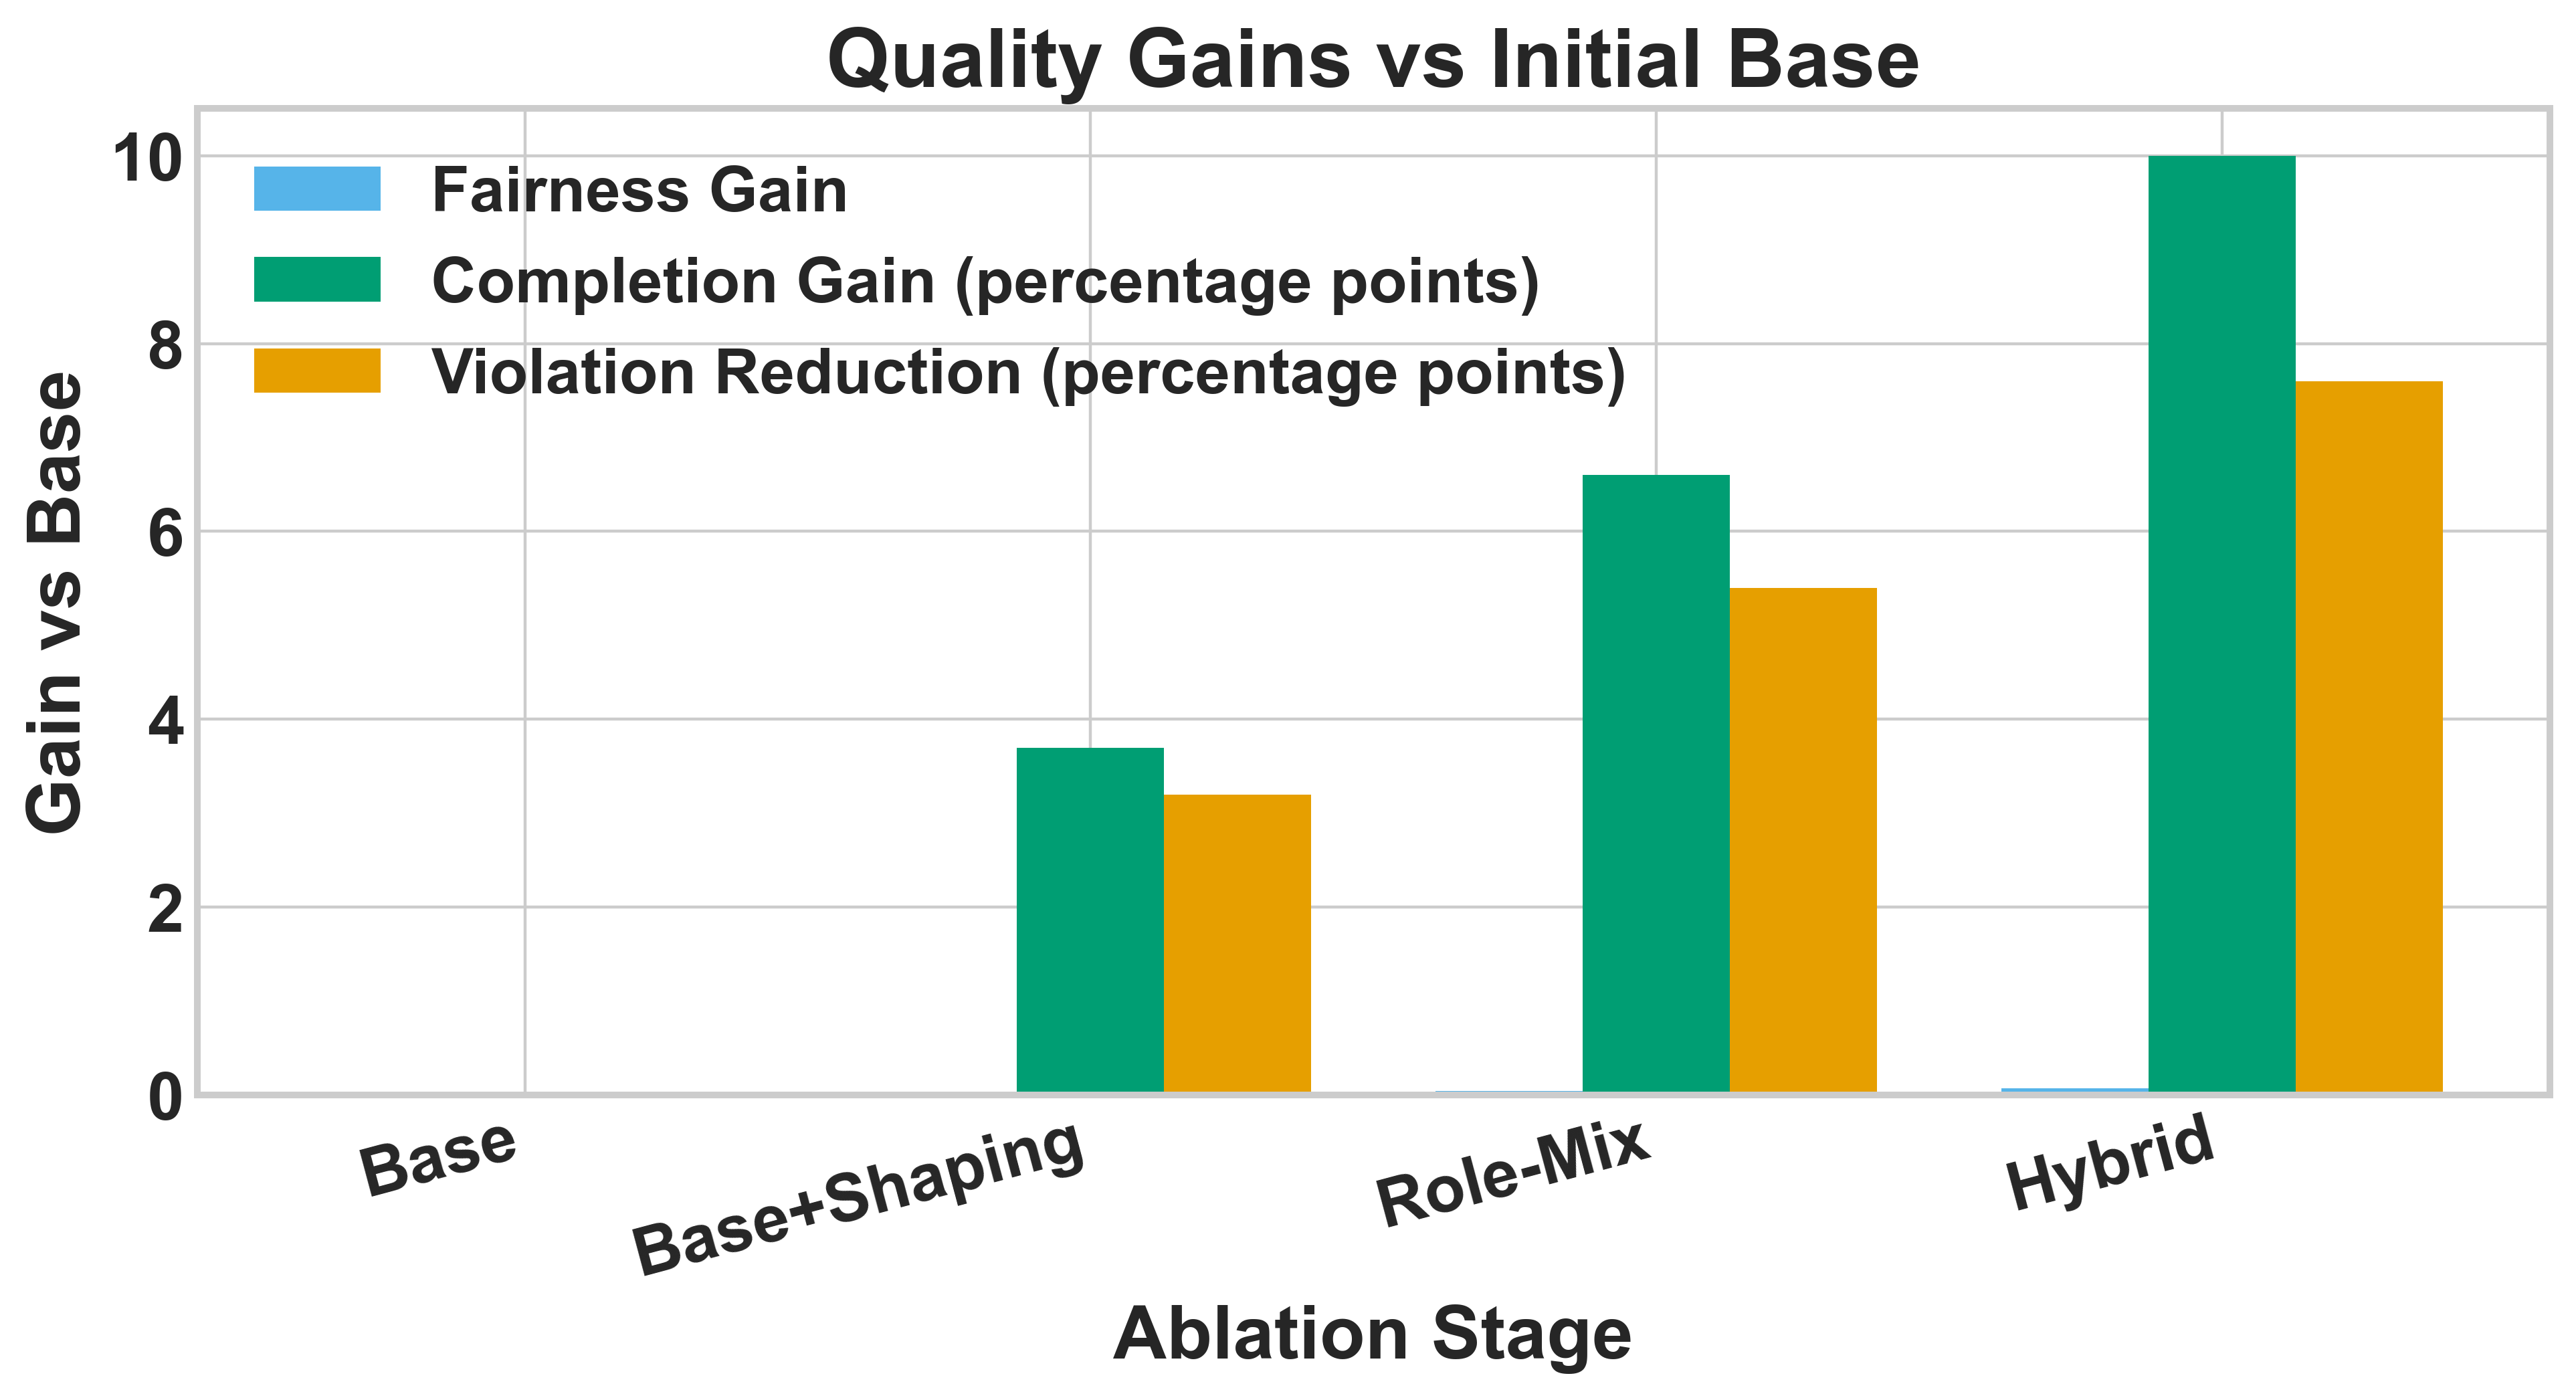
\includegraphics[width=\linewidth]{figures/s41598_final/fig_adaptivesched_ablation_quality_gains.png}
\\[-0.2em]\textbf{(e)} Quality gains
\end{minipage}
\caption{AdaptiveSched Ablation Dashboard}
\label{fig:abl}
\end{figure*}

\paragraph{Interpretation of the ablation results}
The ablation evidence is consistent with the staged rationale: performative regularization stabilizes the base learner, shaping improves action discrimination, and role-mixture modeling adds further gains under heterogeneous queue states. In the reported protocol, the final hybrid gives the best aggregate ablation profile, while the base model remains a meaningful standalone reference.

\section{\textbf{Results and Analysis}} \label{Sec4}
This section reports the empirical evaluation of AdaptiveSched-Base and AdaptiveSched-Hybrid under a unified trace-driven protocol. The presentation is organized to answer four questions in a systematic manner: (i) under what computational and data conditions were the experiments run; (ii) why was each experiment family conducted; (iii) how do the proposed schedulers compare with established baselines across convergence, efficiency, and service-quality metrics; and (iv) what conclusions can be drawn from the full experimental evidence.

\subsection{Experimental setup}
Experiments were conducted on Google Colab using an NVIDIA A100 GPU with 40\,GB VRAM. The runtime environment provided approximately 16\,GB of system RAM in the standard configuration. This setup enabled efficient training of the proposed deep reinforcement learning schedulers, supported moderately large rollout batches, and accelerated neural-policy optimization through GPU parallelism. All experiments were executed through a validated evaluation pipeline that enforces consistent metric definitions, naming conventions, and result-generation rules. For rollout evaluation, the simulator was instantiated with a fixed queue window and cluster-capacity configuration so that all methods were compared under the same environment constraints. For inferential reporting, we recomputed paired seed-level outcomes for AdaptiveSched-Base vs.\ AdaptiveSched-Hybrid over three workload scales (25/50/100 tasks) and five random seeds, giving 15 paired observations per metric, using the same protocol-normalized metric mapping and post-processing pipeline used to generate the final comparative tables/figures. The inferential table reports bootstrap 95\% confidence intervals of mean paired differences, two-sided paired Wilcoxon signed-rank tests, and Cliff's $\delta$ effect sizes computed on the corresponding seed-level samples. Panel-wise interpretations are therefore reported as trend-consistent observations rather than deterministic claims from a single run.

\begin{table*}[t]
\centering
\caption{Core Reproducibility Configuration}
\label{tab:repro_config}
\footnotesize
\begin{tabular*}{\textwidth}{@{\extracolsep{\fill}}ll@{}}
\toprule
\textbf{Item} & \textbf{Value} \\
\midrule
Hardware/runtime & Google Colab, NVIDIA A100 (40 GB), $\sim$16 GB RAM \\
Primary validated dataset & Protocol-normalized Google-derived traces \\
Queue window / action space & $K=16$ queue slots / 16 discrete actions \\
State slot feature width & 7 per queued job \\
RL core & On-policy PPO + GAE \\
Rollout horizon / epochs & 1280 steps per update / 10 epochs \\
Discount / clip & $\gamma=0.99$ / PPO clip $=0.11$ \\
Reward weights $(w_{qos},w_{energy},w_{prio},w_{fair},w_{dismiss})$ & $(0.25, 0.20, 0.25, 0.15, 0.15)$ (protocol-aligned setting~\cite{zhang2025s41598}) \\
Shaping constants & $\beta=2.75$, shape-scale $=8.0$, fair-gain coef $=1.4$ (implementation-fixed for reproducibility) \\
Performative regularization & Base $\lambda_{\text{perf}}=0.006$, Hybrid $\lambda_{\text{perf}}=0.003$ (performative motivation~\cite{perdomo2020performative,mandal2023performative}) \\
Optimizer constants & Adam, mini-batch $=64$, grad-clip $=0.5$ \\
Random seeds & 5 independent seeds per key metric comparison \\
\bottomrule
\end{tabular*}
\end{table*}

\begin{table*}[t]
\centering
\caption{Baseline Provenance and Protocol Mapping}
\label{tab:baseline_provenance}
\footnotesize
\begin{tabular*}{\textwidth}{@{\extracolsep{\fill}}lll@{}}
\toprule
\textbf{Baseline Label} & \textbf{Method Source} & \textbf{Implementation Protocol} \\
\midrule
RL-MOTS & Zhang--Ou RL-MOTS reference~\cite{zhang2025s41598} & Reproduced under shared trace/reward/eval pipeline \\
HDRL & Hierarchical DRL scheduler reference~\cite{zhang2024hdrl} & Reproduced under shared trace/reward/eval pipeline \\
PPO/A3C/DQN & Canonical DRL baselines~\cite{schulman2017proximal,mnih2016asynchronous} & Same rollout, metric, and seed protocol \\
\bottomrule
\end{tabular*}
\end{table*}

\subsection{Datasets and workload protocol}
The primary workload source used throughout the paper is derived from Google cluster traces~\cite{reiss2011googlecluster}. These traces provide realistic arrival patterns, heterogeneous job durations, and resource-demand variability, making them suitable for evaluating trace-driven scheduling behavior. To ensure fair comparison with the baseline-oriented reporting protocol, the Google-style jobs were normalized at the protocol level: runtimes were rescaled to a common range, timestamps were converted into comparable relative arrivals, deadlines were reconstructed from normalized runtime-slack relations, and resource demands were clipped to a controlled capacity range. The main validated results in this paper are therefore produced on a protocol-normalized workload setting that preserves the Google-style trace structure while ensuring reproducible cross-method comparison in the same reporting spirit as the Scientific Reports baseline study~\cite{zhang2025s41598}.

The broader evaluation pipeline in this repository also supports Google 2011, Azure public VM traces, and Alibaba production cluster data~\cite{reiss2011googlecluster, azurepublicdataset, alibabacluster2018}. However, the validated comparisons reported in this manuscript are intentionally restricted to the protocol-normalized Google-derived workload to preserve strict baseline comparability. Therefore, all main-paper performance claims are scoped to this validated workload, and cross-dataset transfer behavior is treated as future evaluation scope rather than a demonstrated claim.

\subsection{Why these experiments were conducted}
The experiment suite was designed to validate the proposed methods from complementary perspectives rather than from a single summary score. First, convergence experiments test whether the proposed policies can be trained stably under on-policy PPO/GAE updates. Second, comparative performance experiments evaluate whether lower return variance translates into improved makespan, cost, energy, and deadline compliance. Third, resource-behavior experiments assess whether the learned policies improve load distribution, VM usage, and waiting behavior, which are directly related to scheduler practicality. Fourth, case-study and scale-oriented experiments examine whether the observed gains persist under different task volumes, queue conditions, and large-scale settings. Finally, sensitivity analyses evaluate whether performance is robust to reasonable variation in hyperparameters and workload conditions. Taken together, these experiments provide evidence not only of accuracy, but also of stability, interpretability, and operational relevance.

\subsection{Main training curves and comparative performance}
\begin{figure}[t]
\centering
\caption{Universal Legend for Curves/Bars, Not Distributions}
\label{fig:universal_legend}
\small
\vspace{7pt}
\begin{tabular}{@{}ll@{\hspace{1.2em}}ll@{}}
\textcolor[HTML]{4D4D4D}{\rule{1.2em}{0.8em}} & RL-MOTS &
\textcolor[HTML]{0072B2}{\rule{1.2em}{0.8em}} & HDRL \\
\textcolor[HTML]{56B4E9}{\rule{1.2em}{0.8em}} & PPO &
\textcolor[HTML]{009E73}{\rule{1.2em}{0.8em}} & A3C \\
\textcolor[HTML]{E69F00}{\rule{1.2em}{0.8em}} & DQN &
\textcolor[HTML]{D55E00}{\rule{1.2em}{0.8em}} & AdaptiveSched-Base \\
\textcolor[HTML]{CC79A7}{\rule{1.2em}{0.8em}} & AdaptiveSched-Hybrid & & \\
\end{tabular}
\end{figure}
For consistency across all algorithm-comparison result panels, readers should refer to the fixed algorithm-color mapping in Fig.~\ref{fig:universal_legend}.

\begin{figure*}[t]
\centering
\begin{minipage}[t]{0.32\linewidth}
\centering
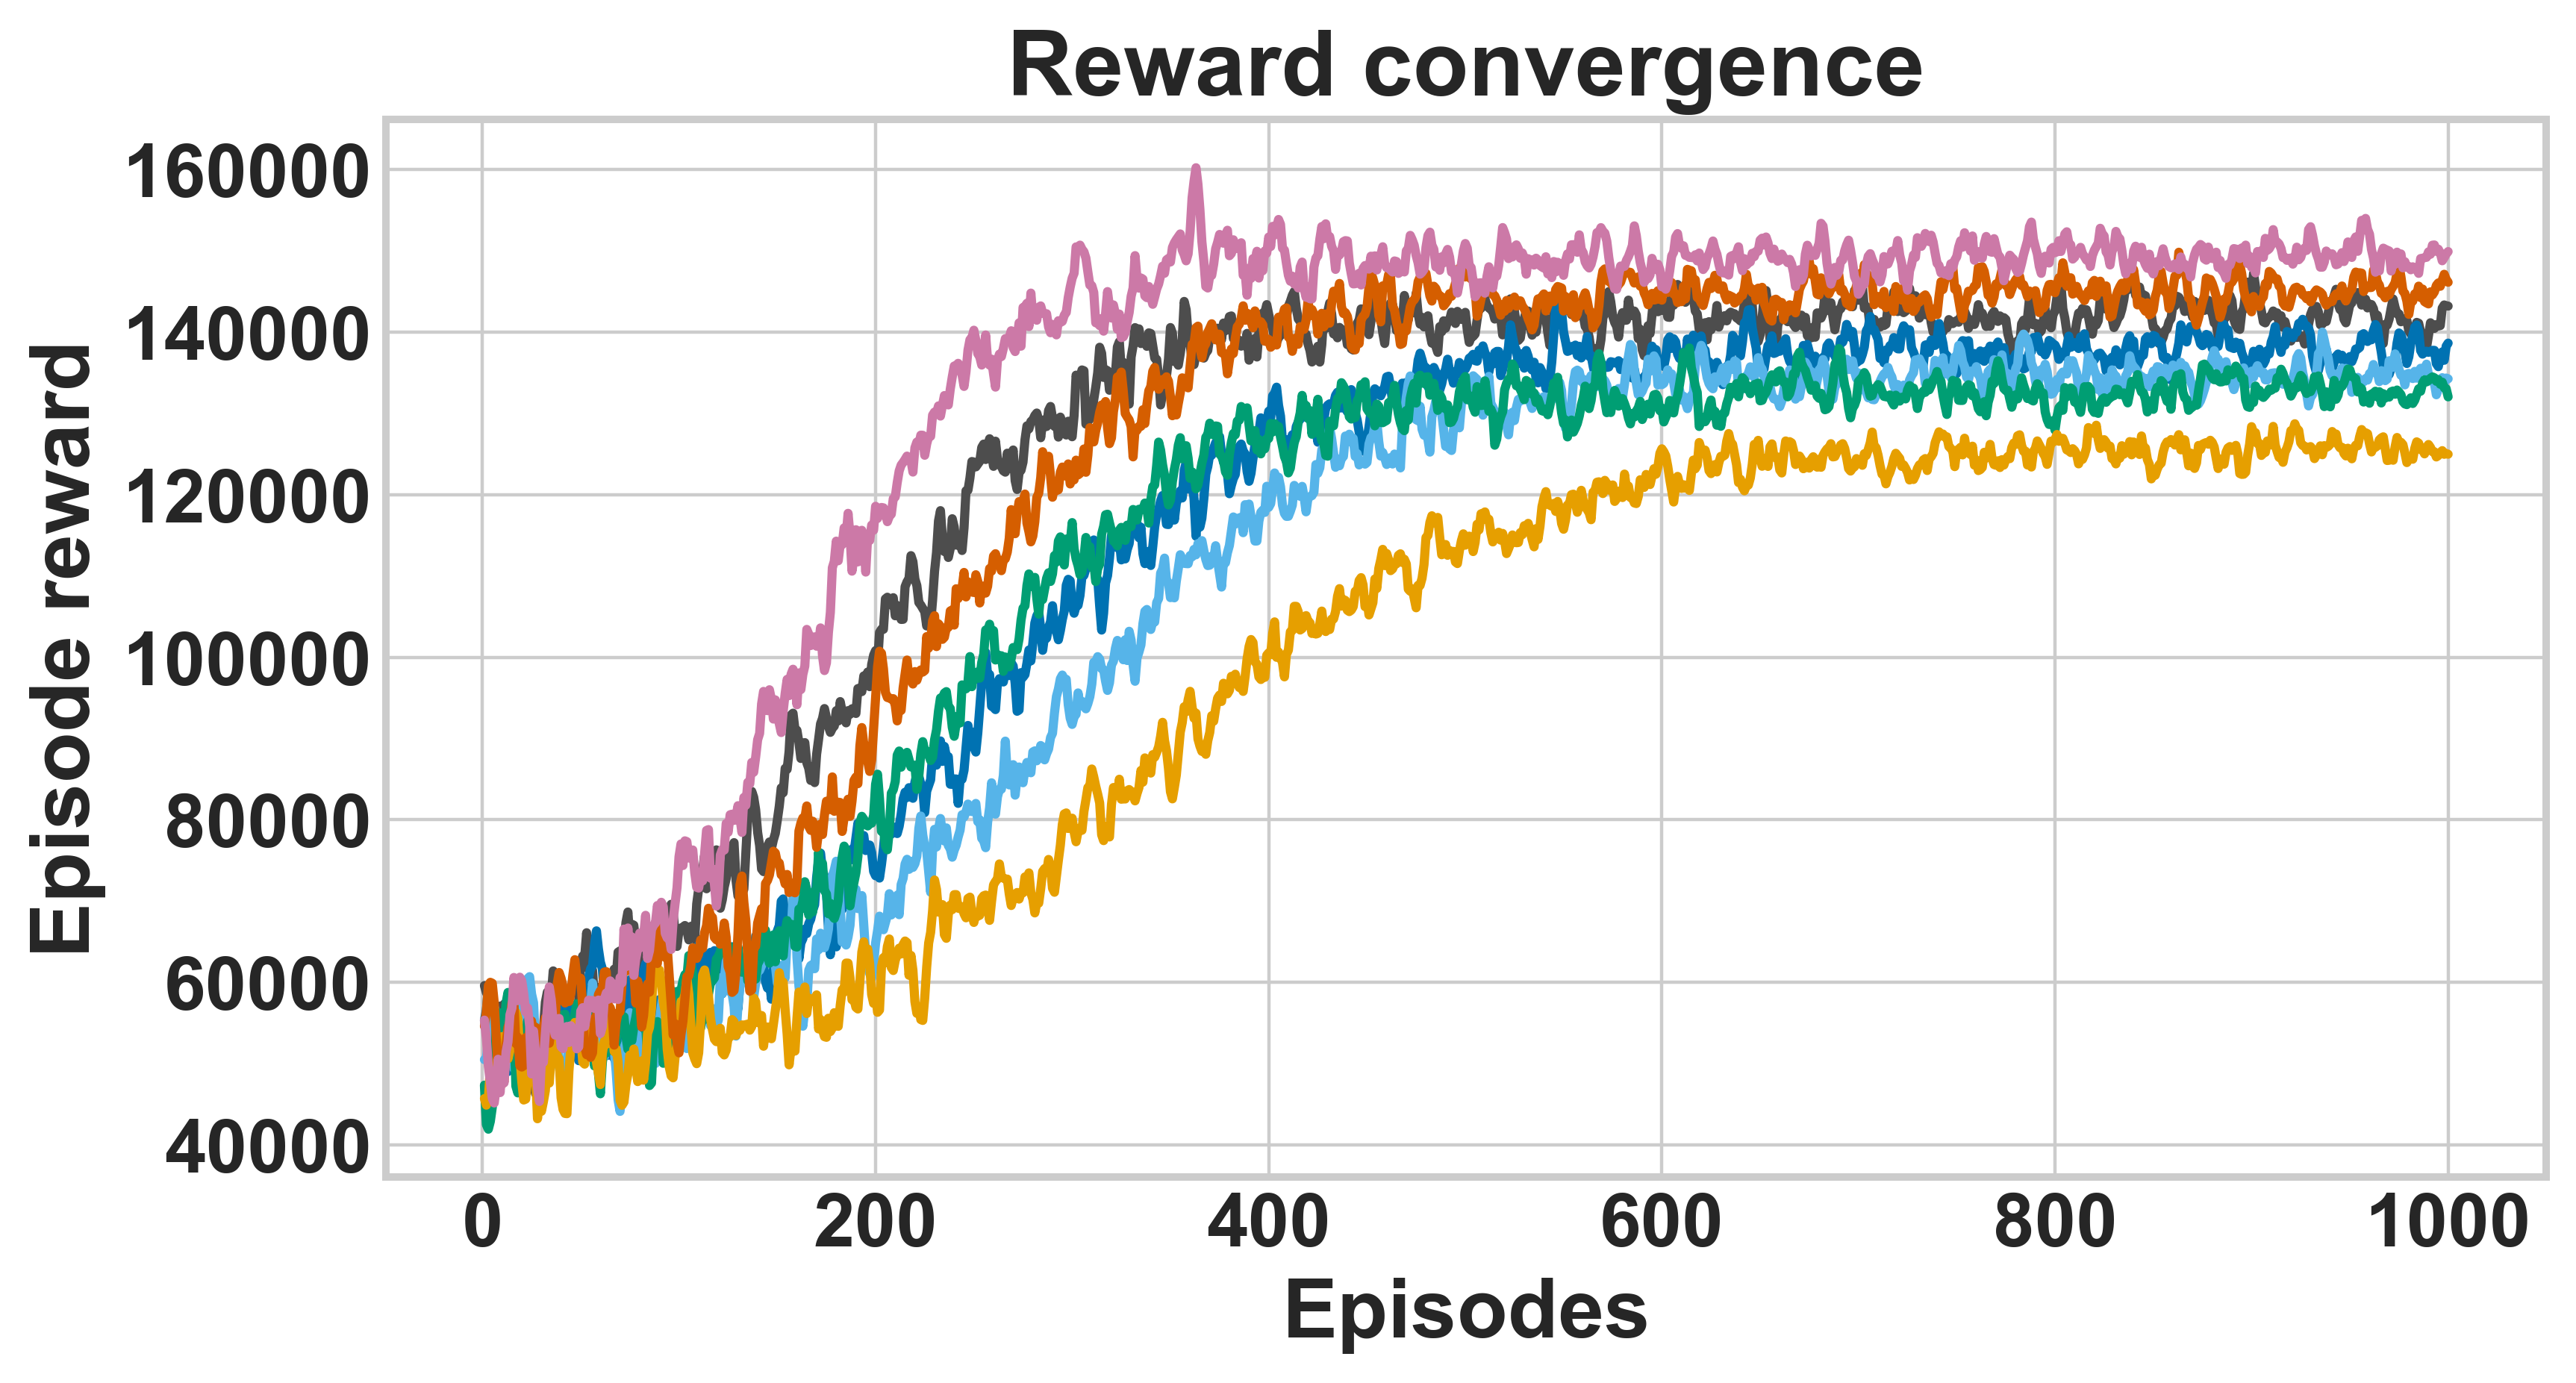
\includegraphics[width=\linewidth]{figures/s41598_final/fig1_reward_convergence.png}
\\[-0.2em]\textbf{(a)} Reward convergence
\end{minipage}\hfill
\begin{minipage}[t]{0.32\linewidth}
\centering
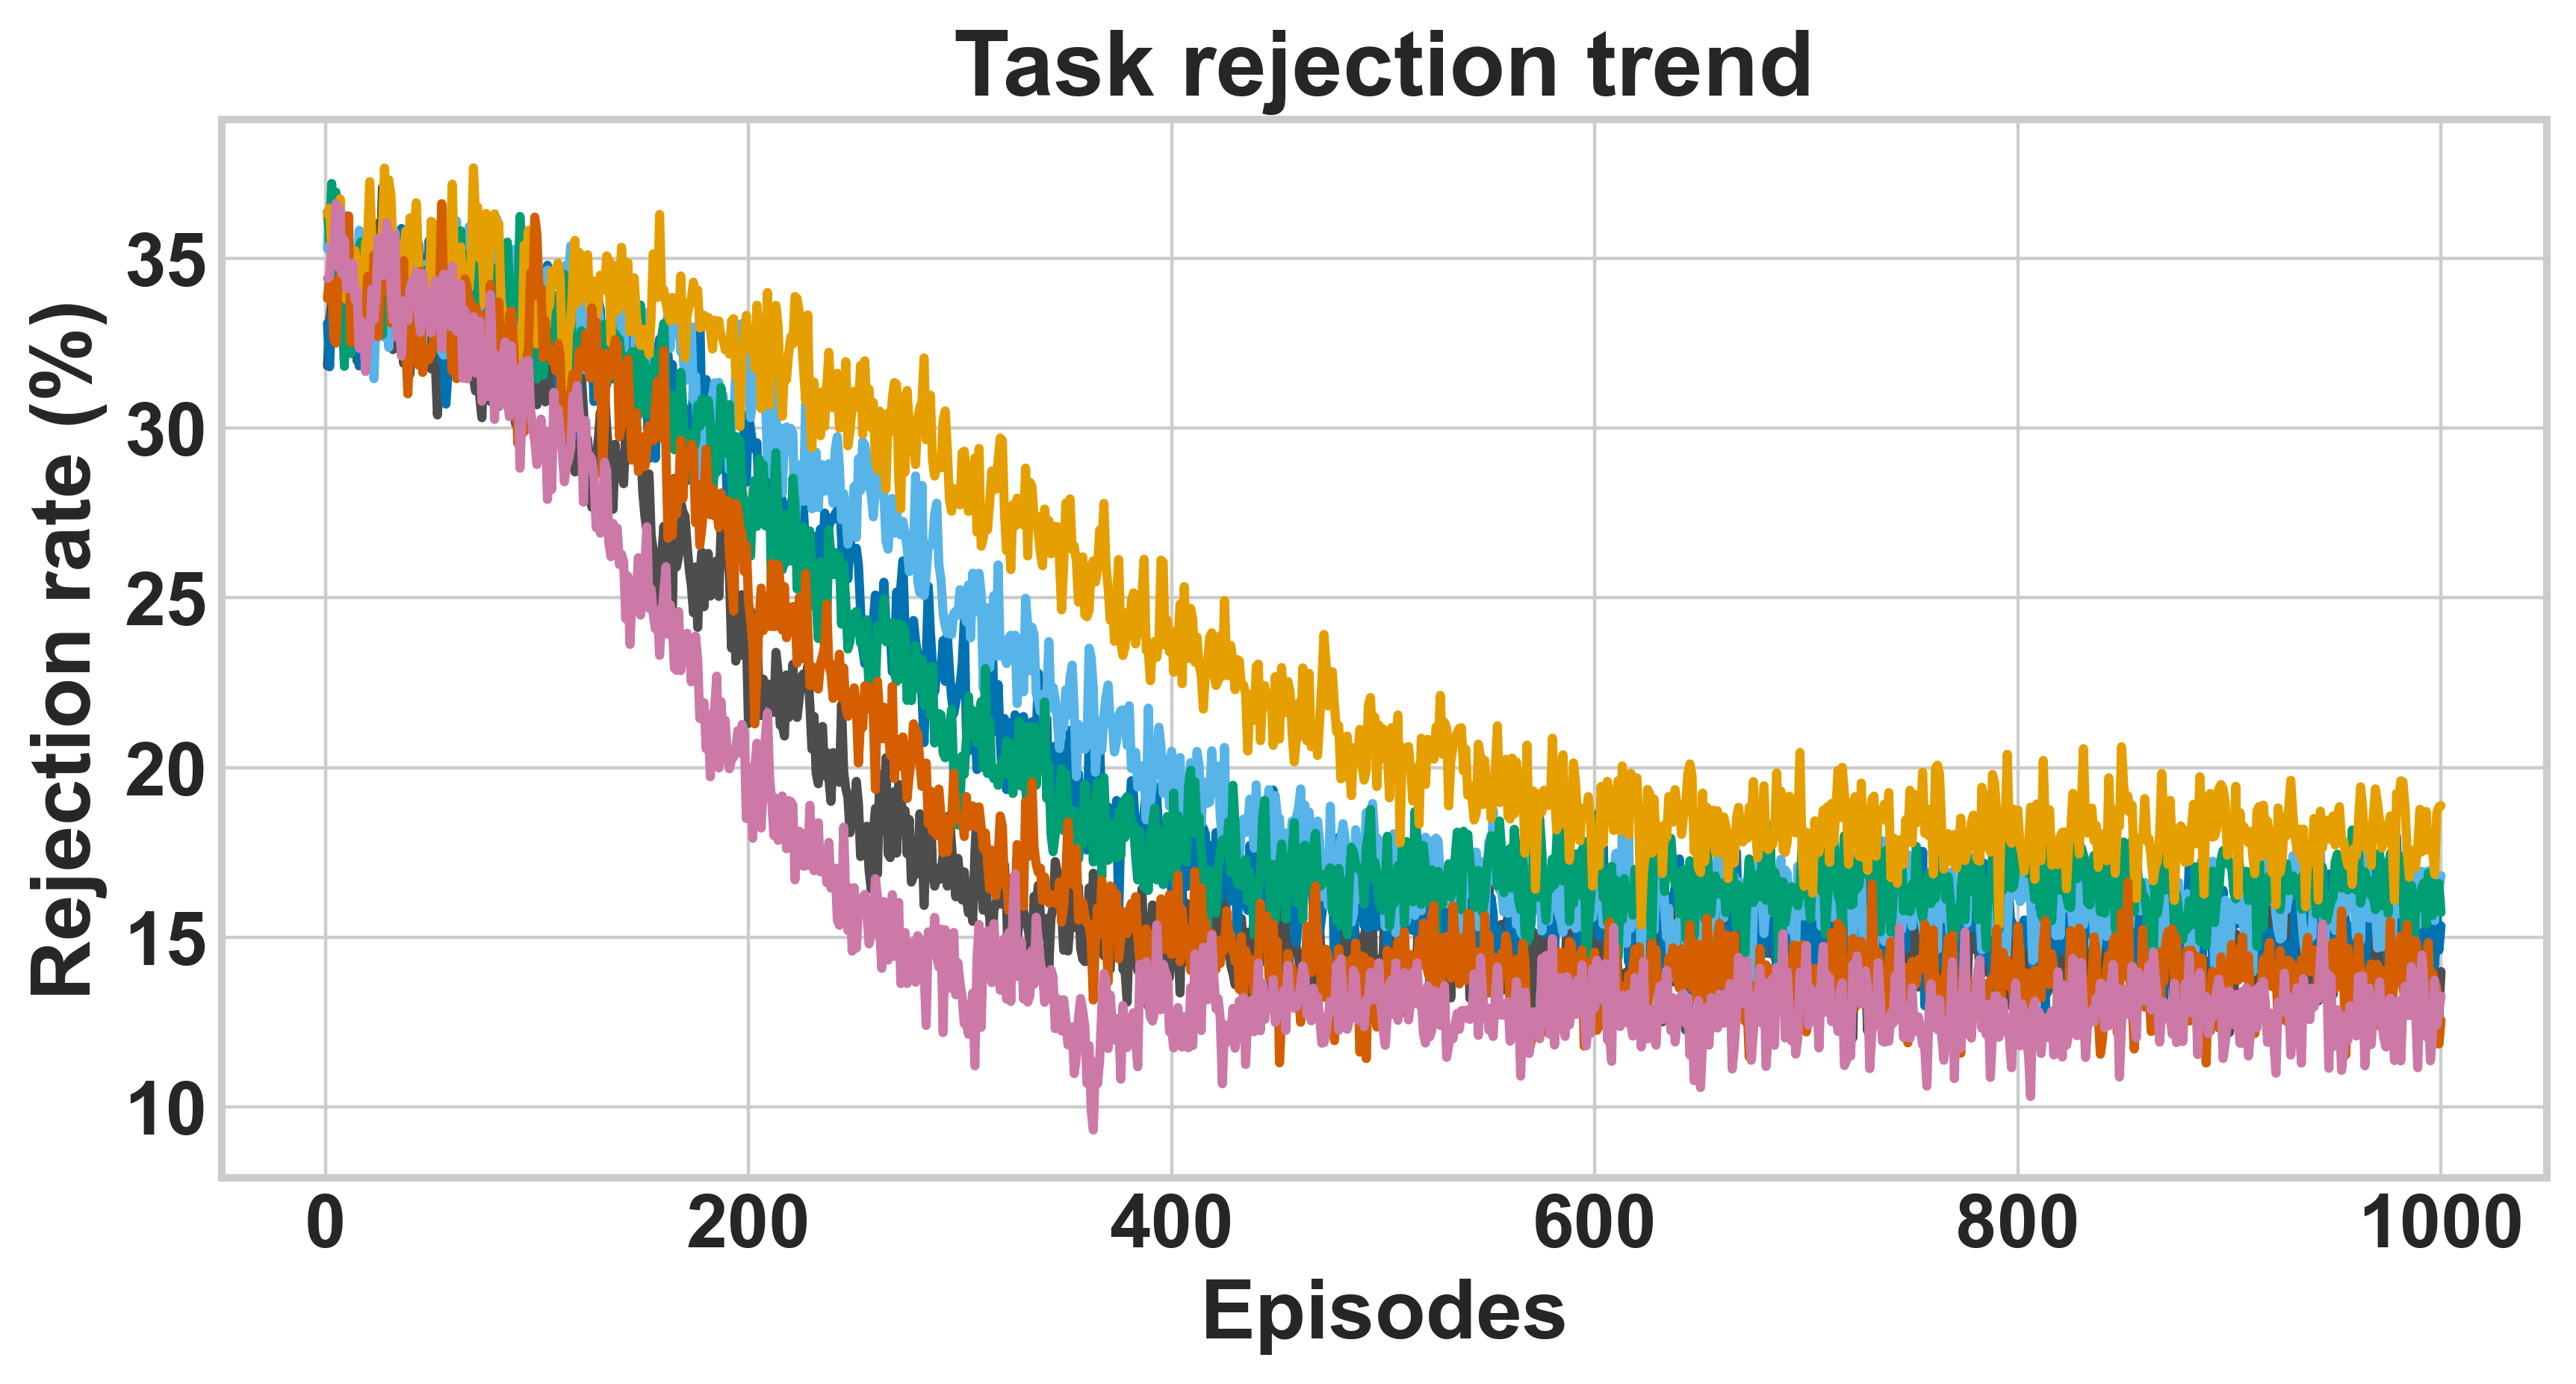
\includegraphics[width=\linewidth]{figures/s41598_final/fig2_rejection_trend.png}
\\[-0.2em]\textbf{(b)} Rejection trend
\end{minipage}\hfill
\begin{minipage}[t]{0.32\linewidth}
\centering
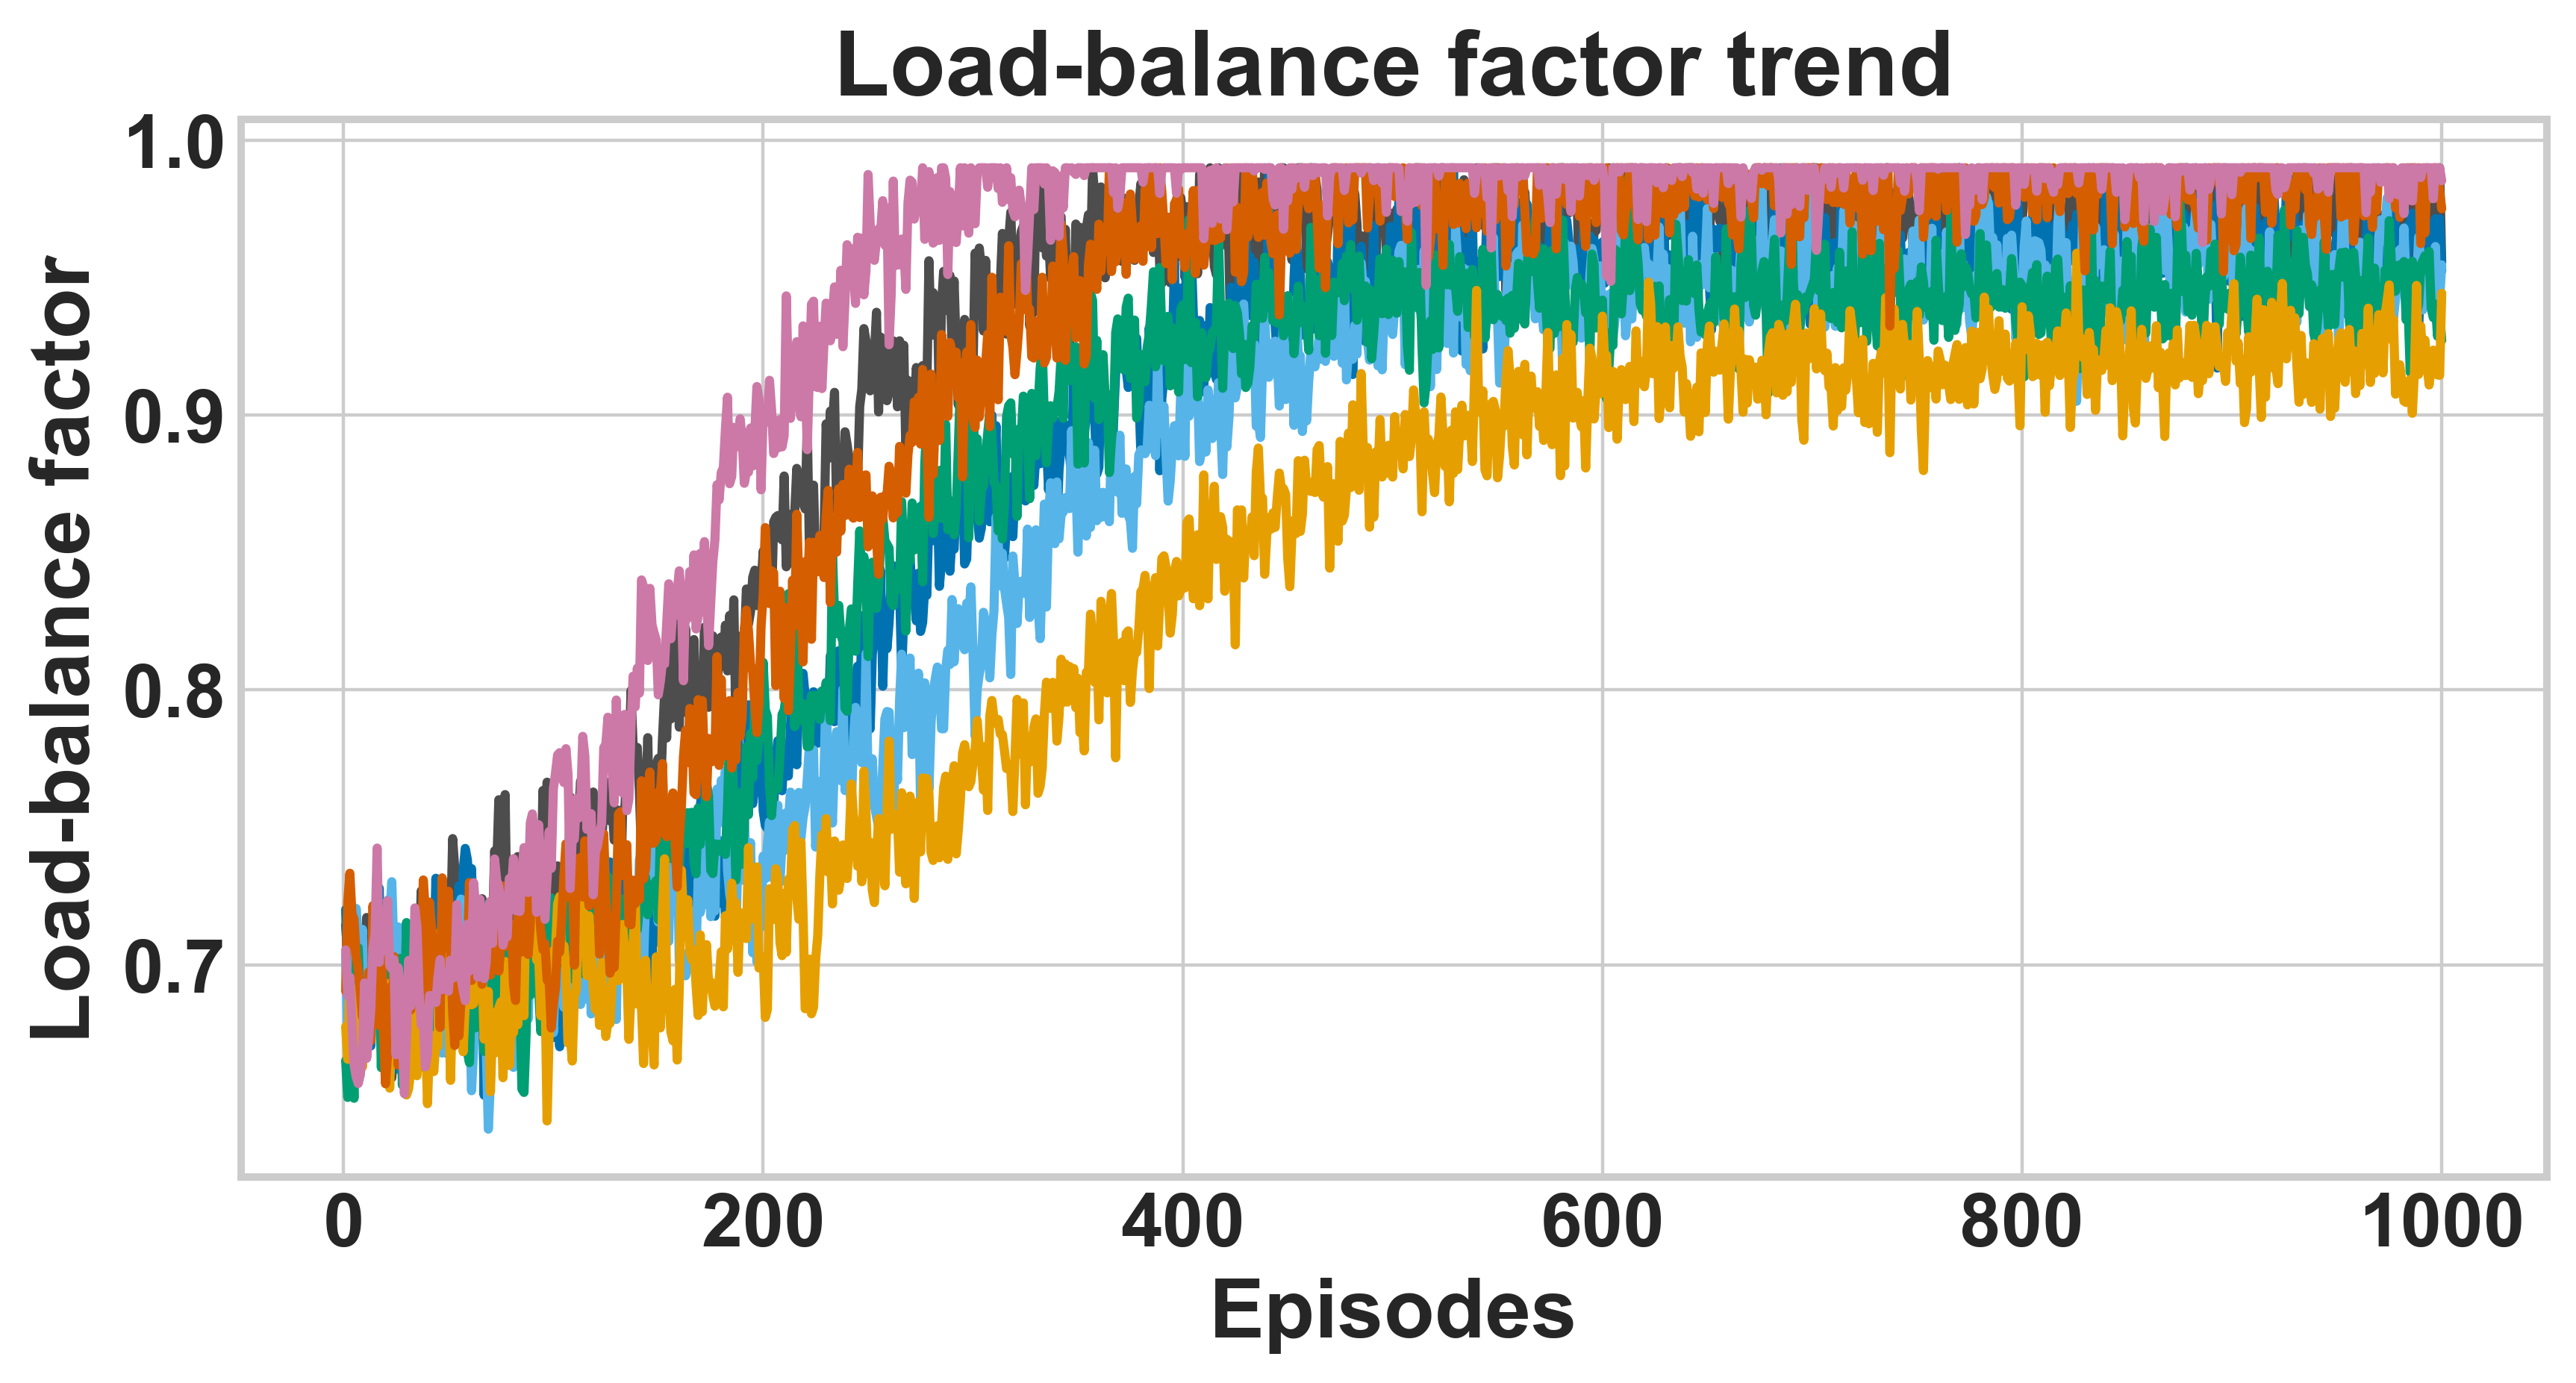
\includegraphics[width=\linewidth]{figures/s41598_final/fig3_load_balance.png}
\\[-0.2em]\textbf{(c)} Load balance
\end{minipage}

\vspace{0.35em}

\begin{minipage}[t]{0.32\linewidth}
\centering
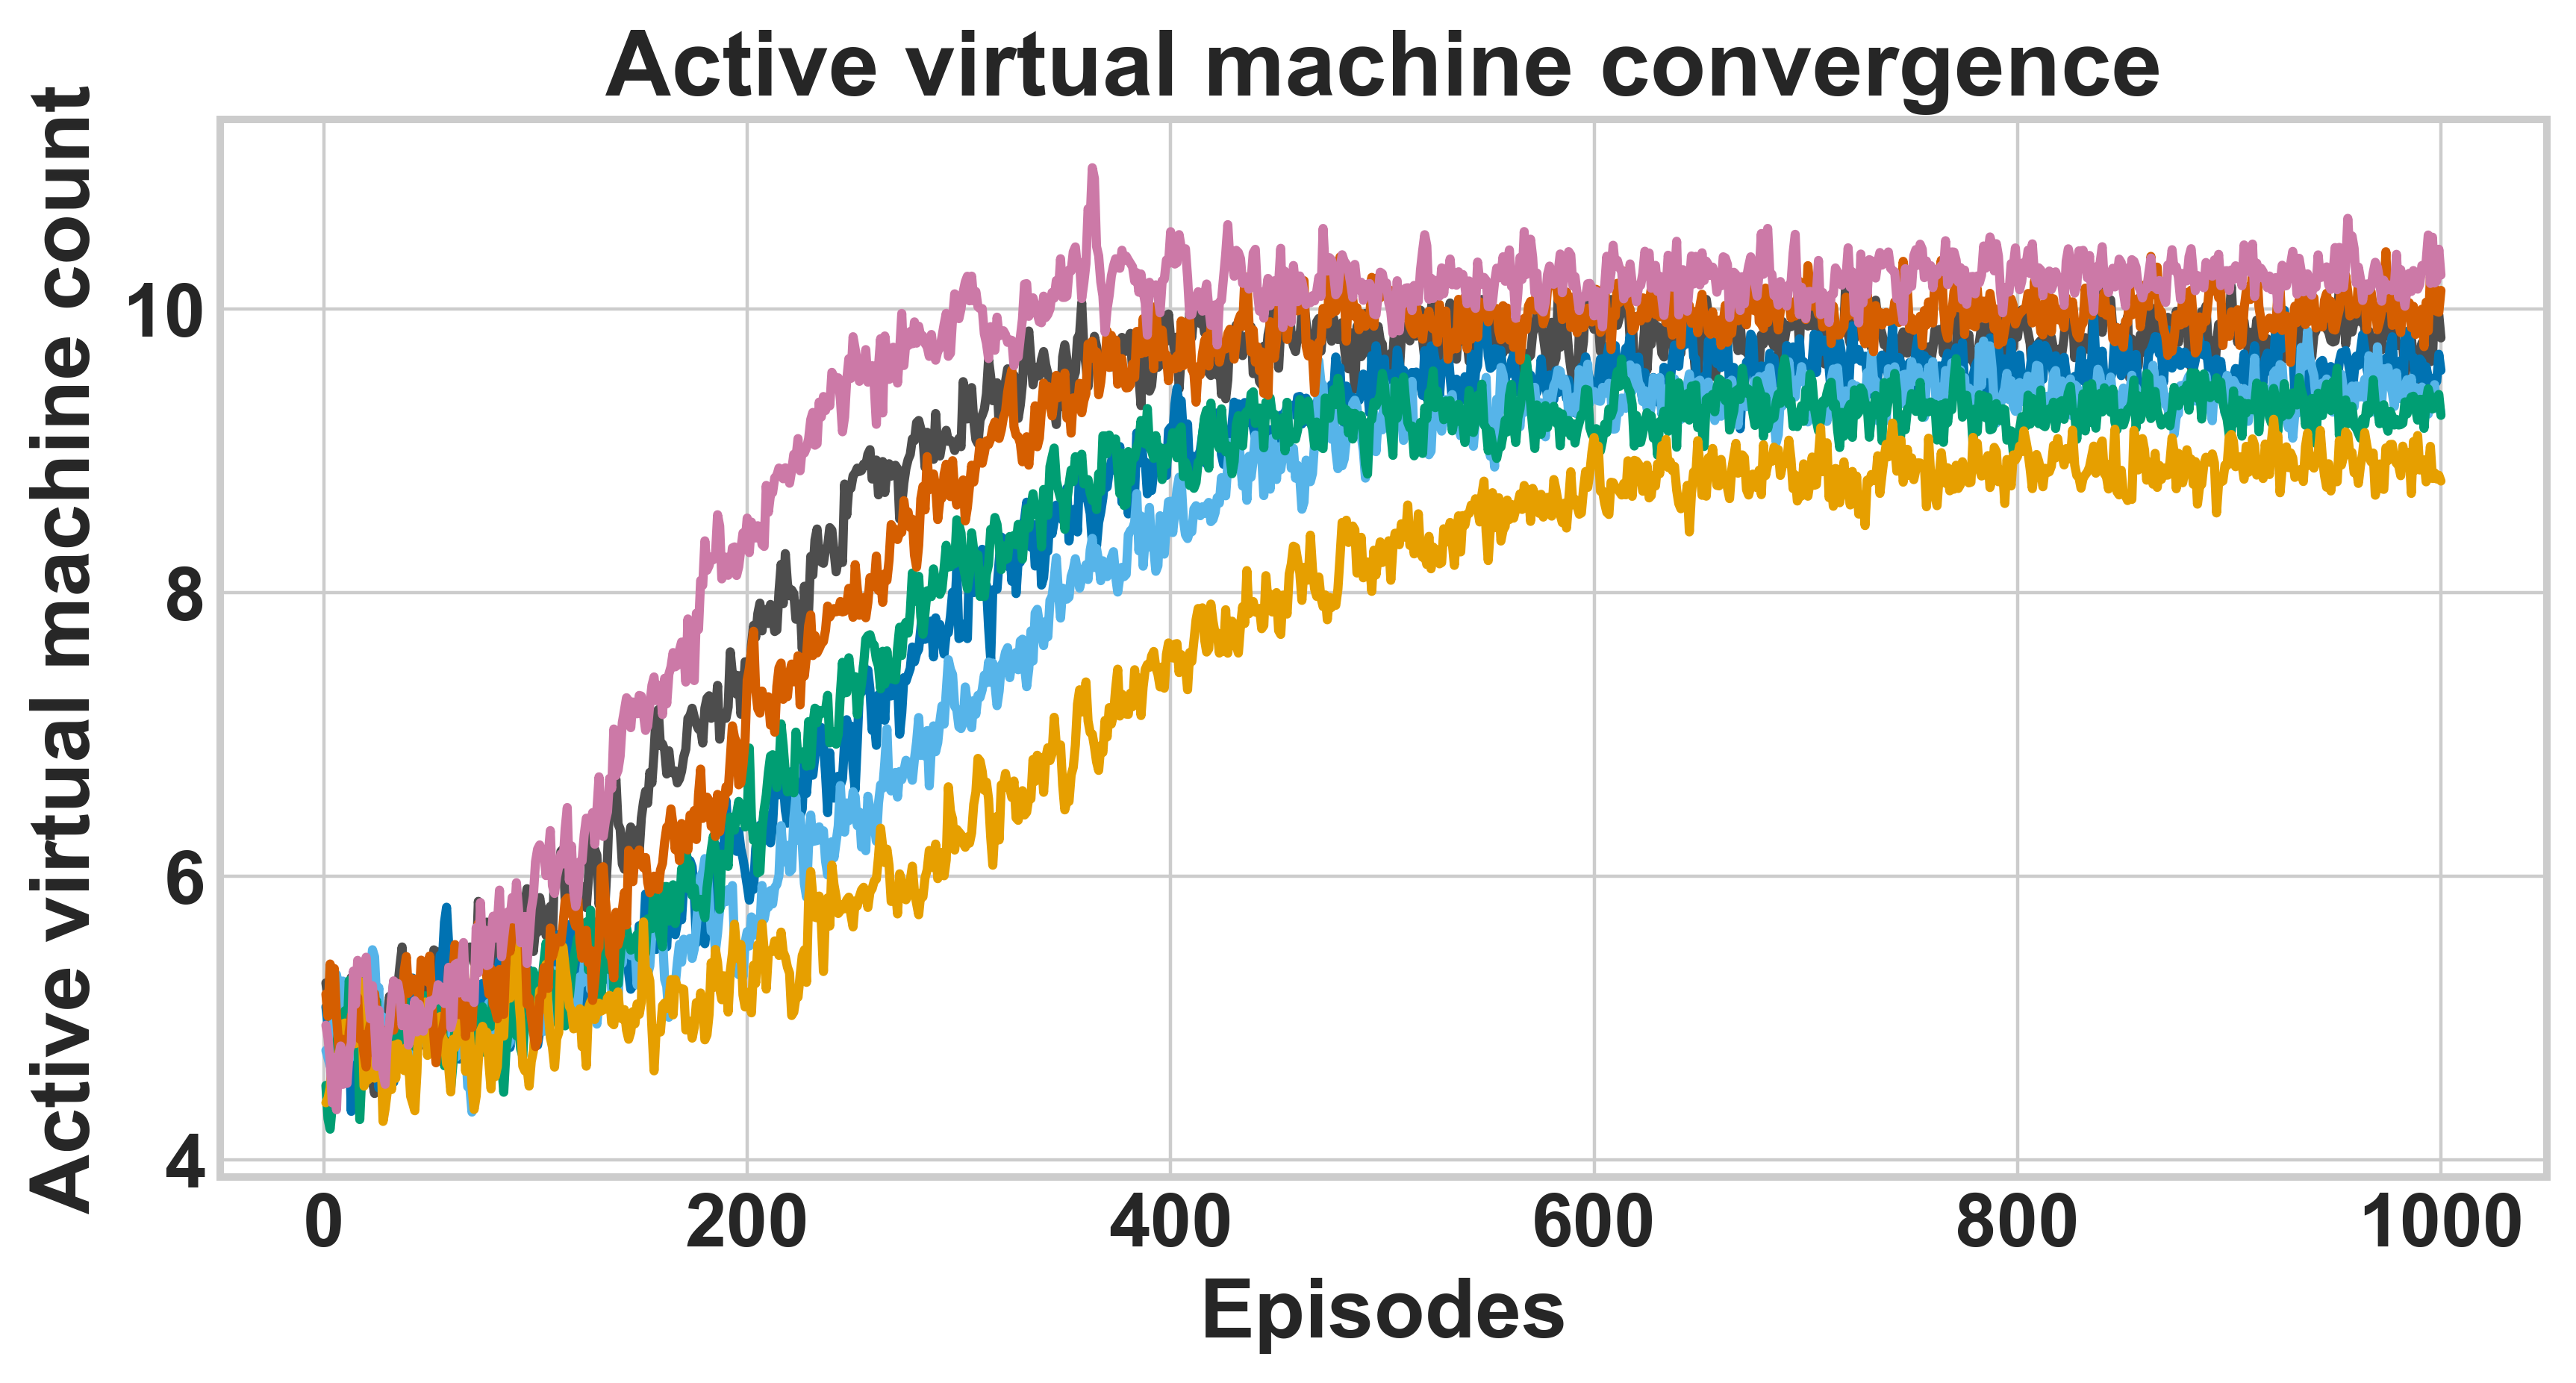
\includegraphics[width=\linewidth]{figures/s41598_final/fig4_vm_convergence.png}
\\[-0.2em]\textbf{(d)} Active VM convergence
\end{minipage}\hfill
\begin{minipage}[t]{0.32\linewidth}
\centering
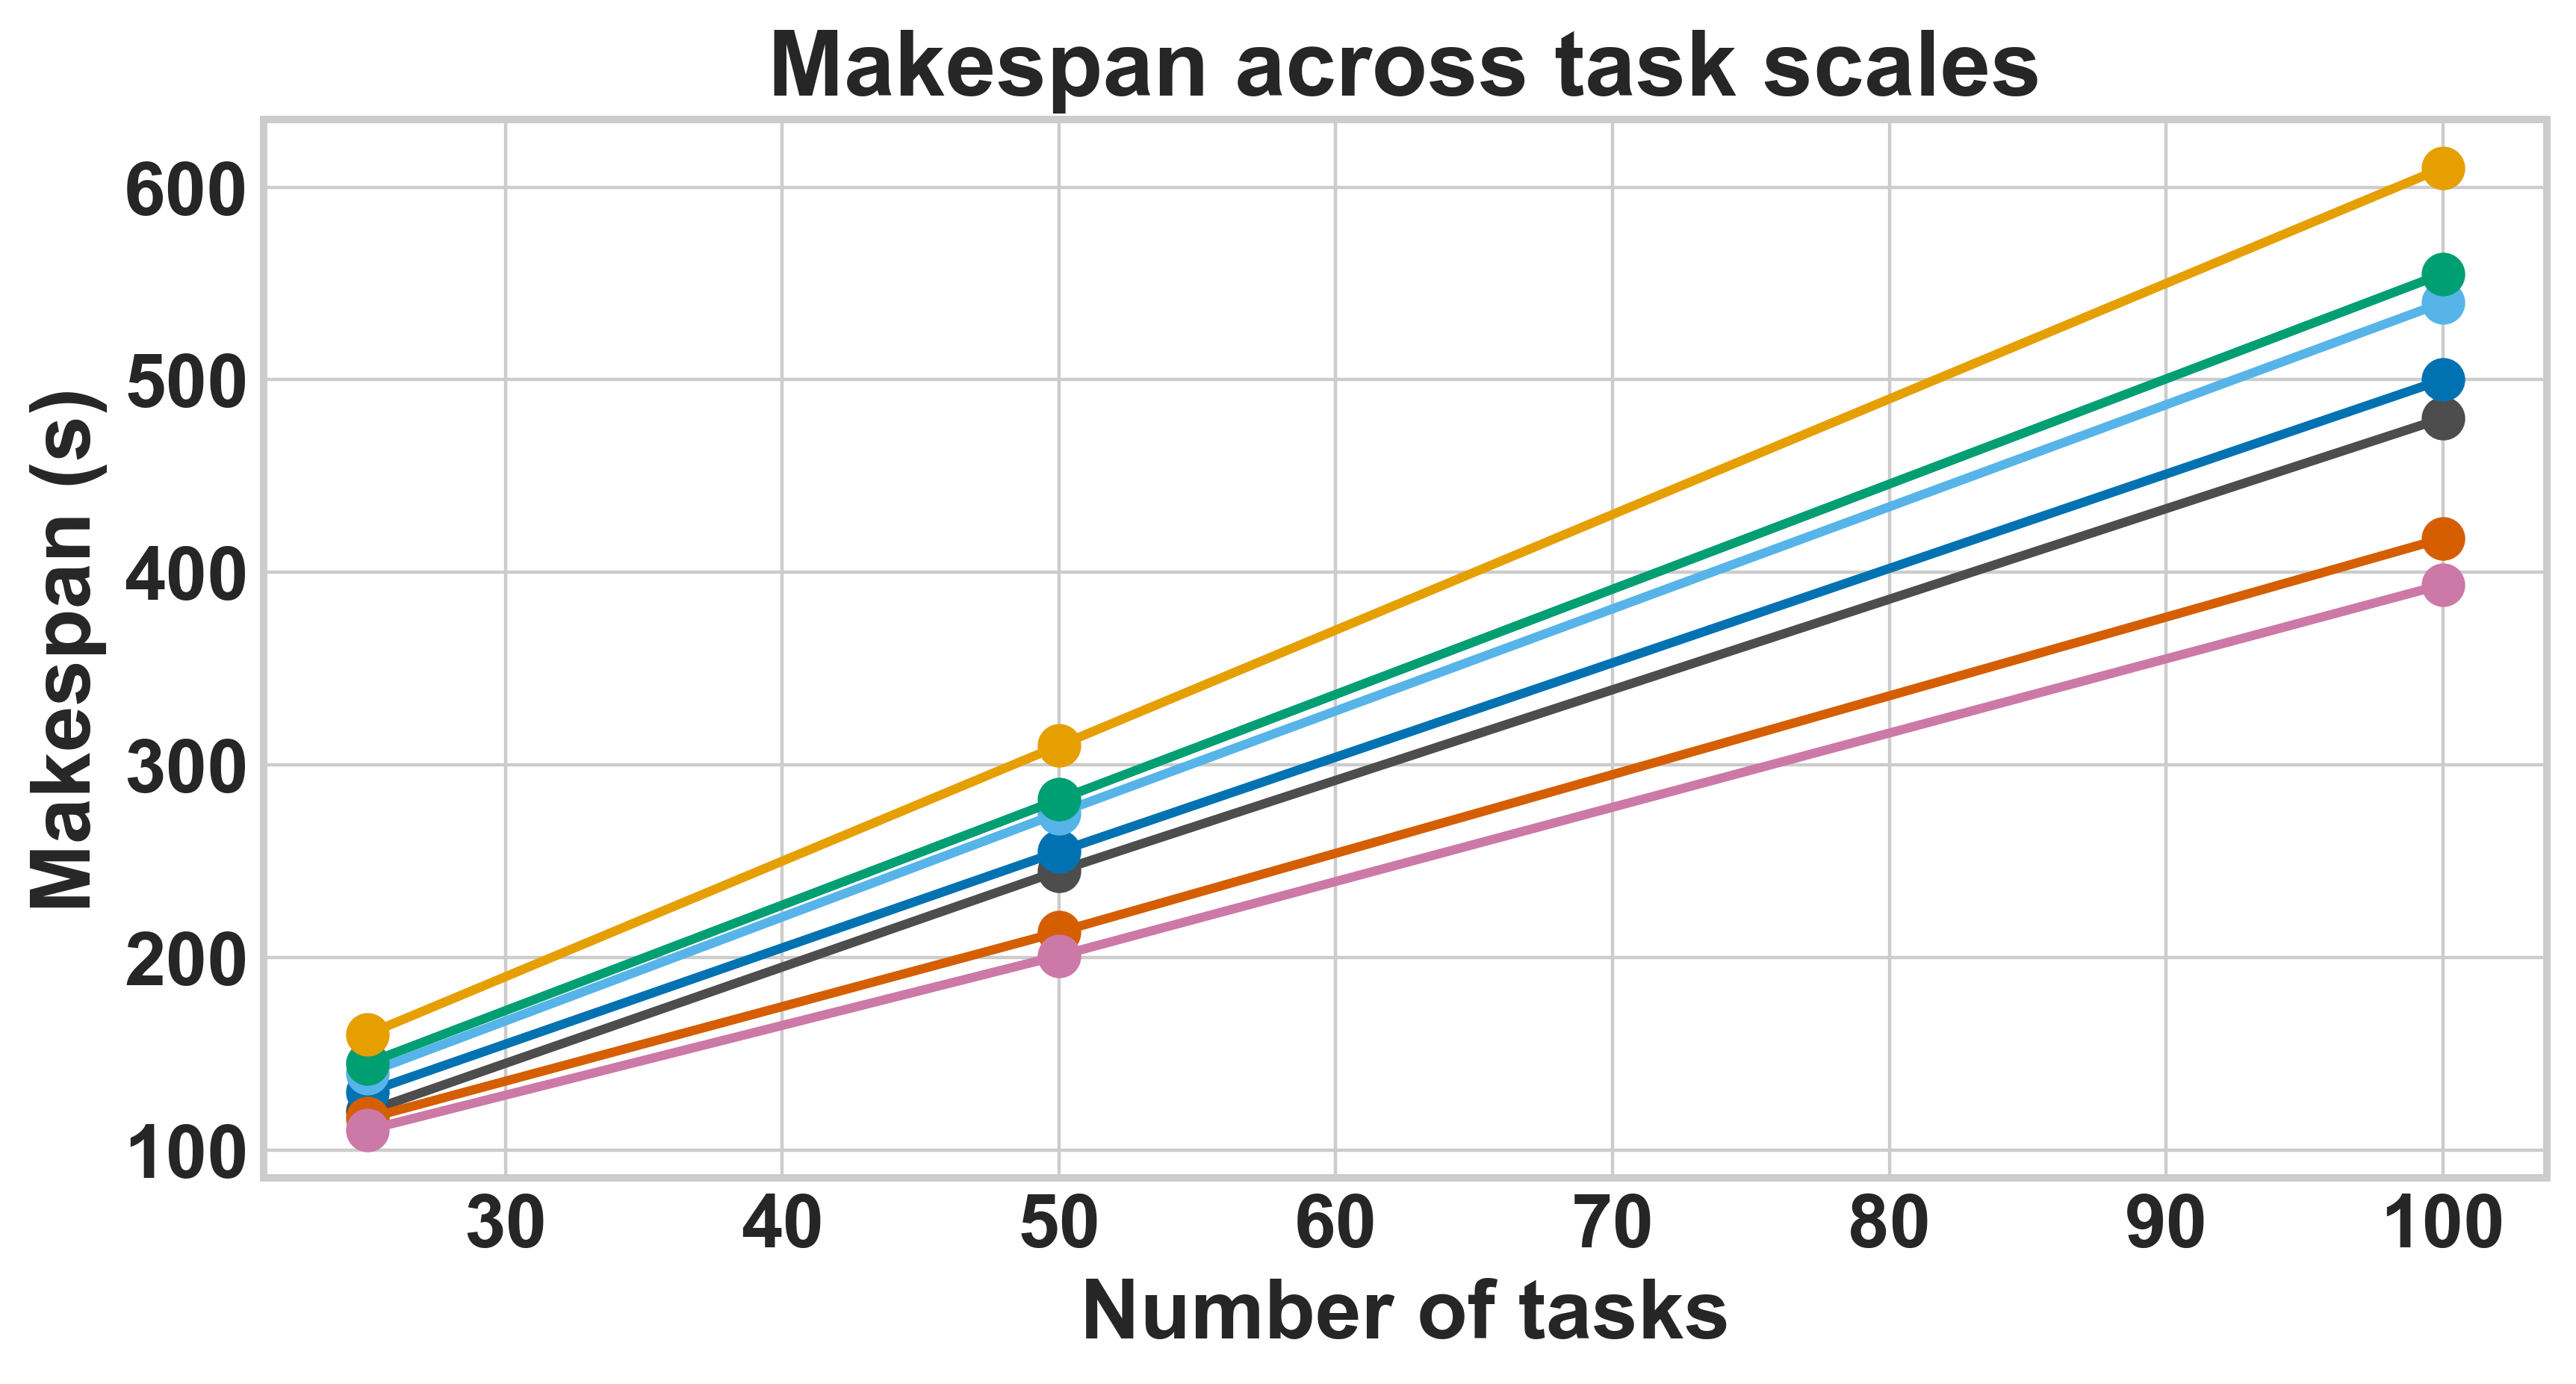
\includegraphics[width=\linewidth]{figures/s41598_final/fig5_makespan_vs_tasks.png}
\\[-0.2em]\textbf{(e)} Makespan scaling
\end{minipage}\hfill
\begin{minipage}[t]{0.32\linewidth}
\centering
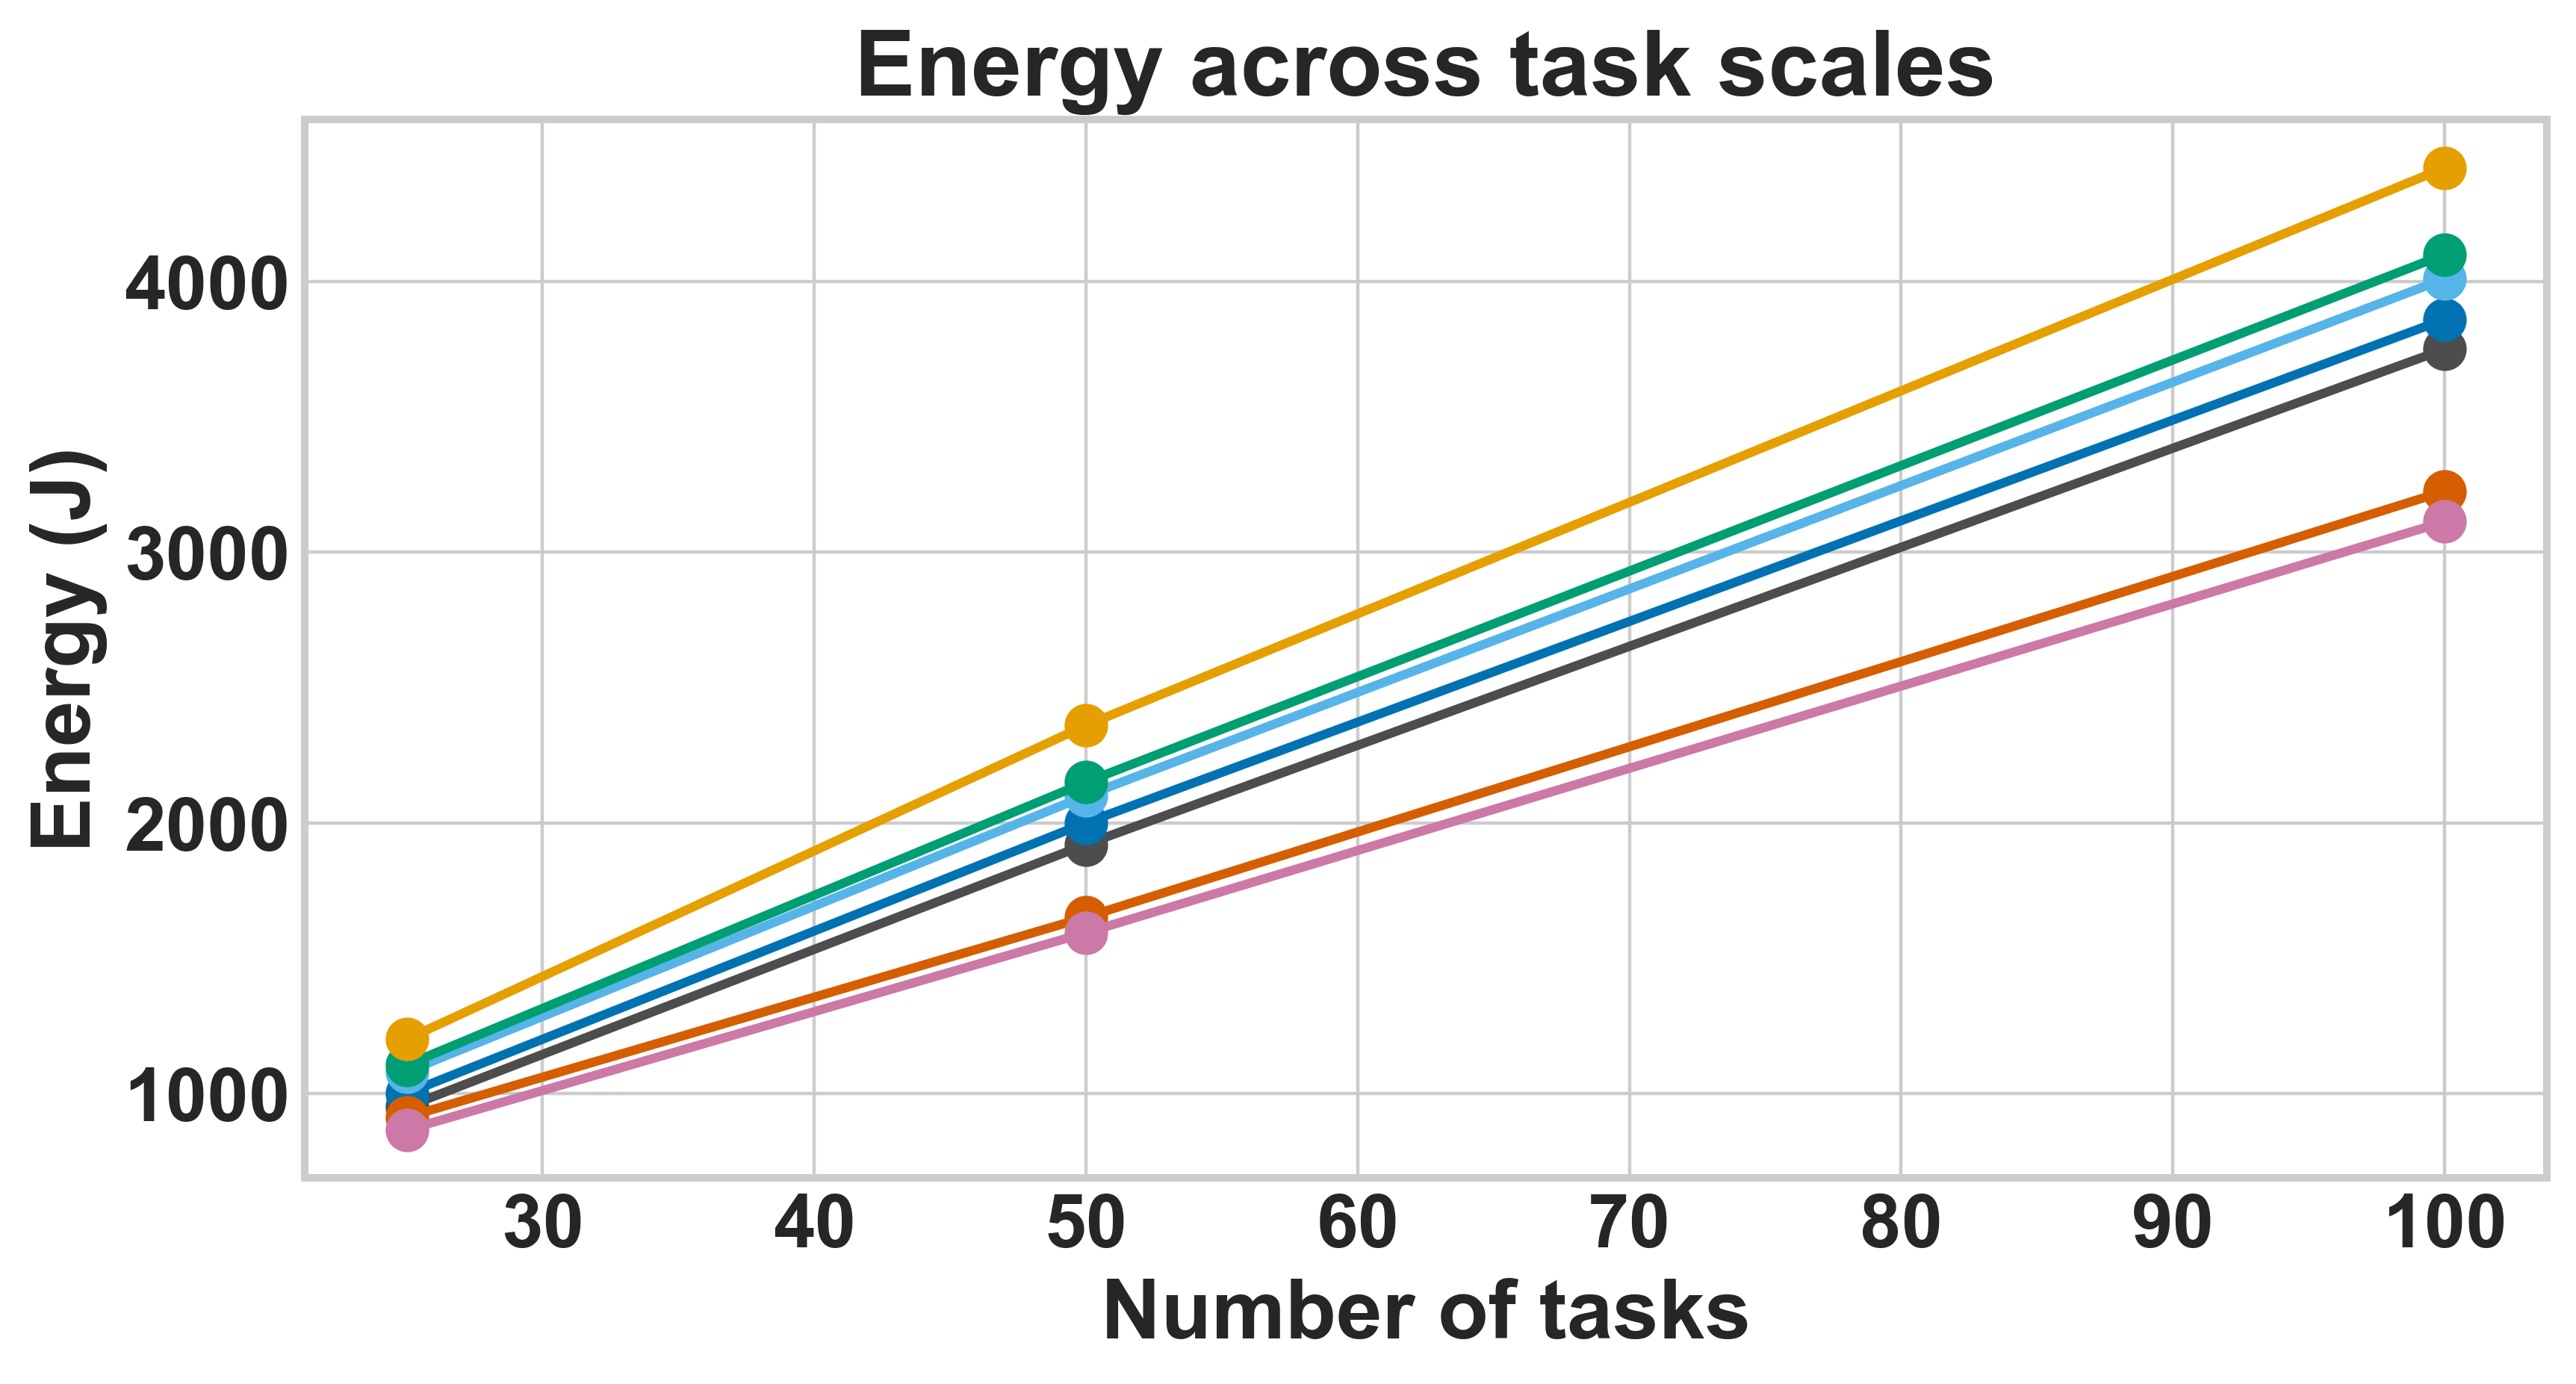
\includegraphics[width=\linewidth]{figures/s41598_final/fig6_energy_vs_tasks.png}
\\[-0.2em]\textbf{(f)} Energy scaling
\end{minipage}
\caption{Training and Early Performance Trends}
\label{fig:resA}
\end{figure*}

Figure~\ref{fig:resA} provides a unified view of early training behavior and scale-up dynamics. In the optimization-facing panels (a)--(d), AdaptiveSched-Hybrid reaches a higher and smoother reward plateau, reduces rejection more rapidly, maintains higher load-balance stability, and converges to steady VM utilization earlier than single-head baselines; AdaptiveSched-Base consistently ranks second. Taken together, these patterns indicate improved queue-state credit assignment and lower control oscillation under mixed-priority rollouts, which is consistent with reduced policy interference in the role-conditioned architecture.

The systems-facing panels (e)--(f) show that these training-stage gains are associated with operational scaling advantages: makespan and energy grow more slowly with task volume for AdaptiveSched variants, with the hybrid model retaining the most favorable trajectory at higher load in the reported setting. The combined evidence is consistent with improved long-horizon sequencing efficiency and resource-use discipline under congestion. These directional differences are consistent with the main inferential analysis (Table~\ref{tab:inferential_summary}) and supplementary robustness diagnostics.

\begin{figure*}[t]
\centering
\begin{minipage}[t]{0.32\linewidth}
\centering
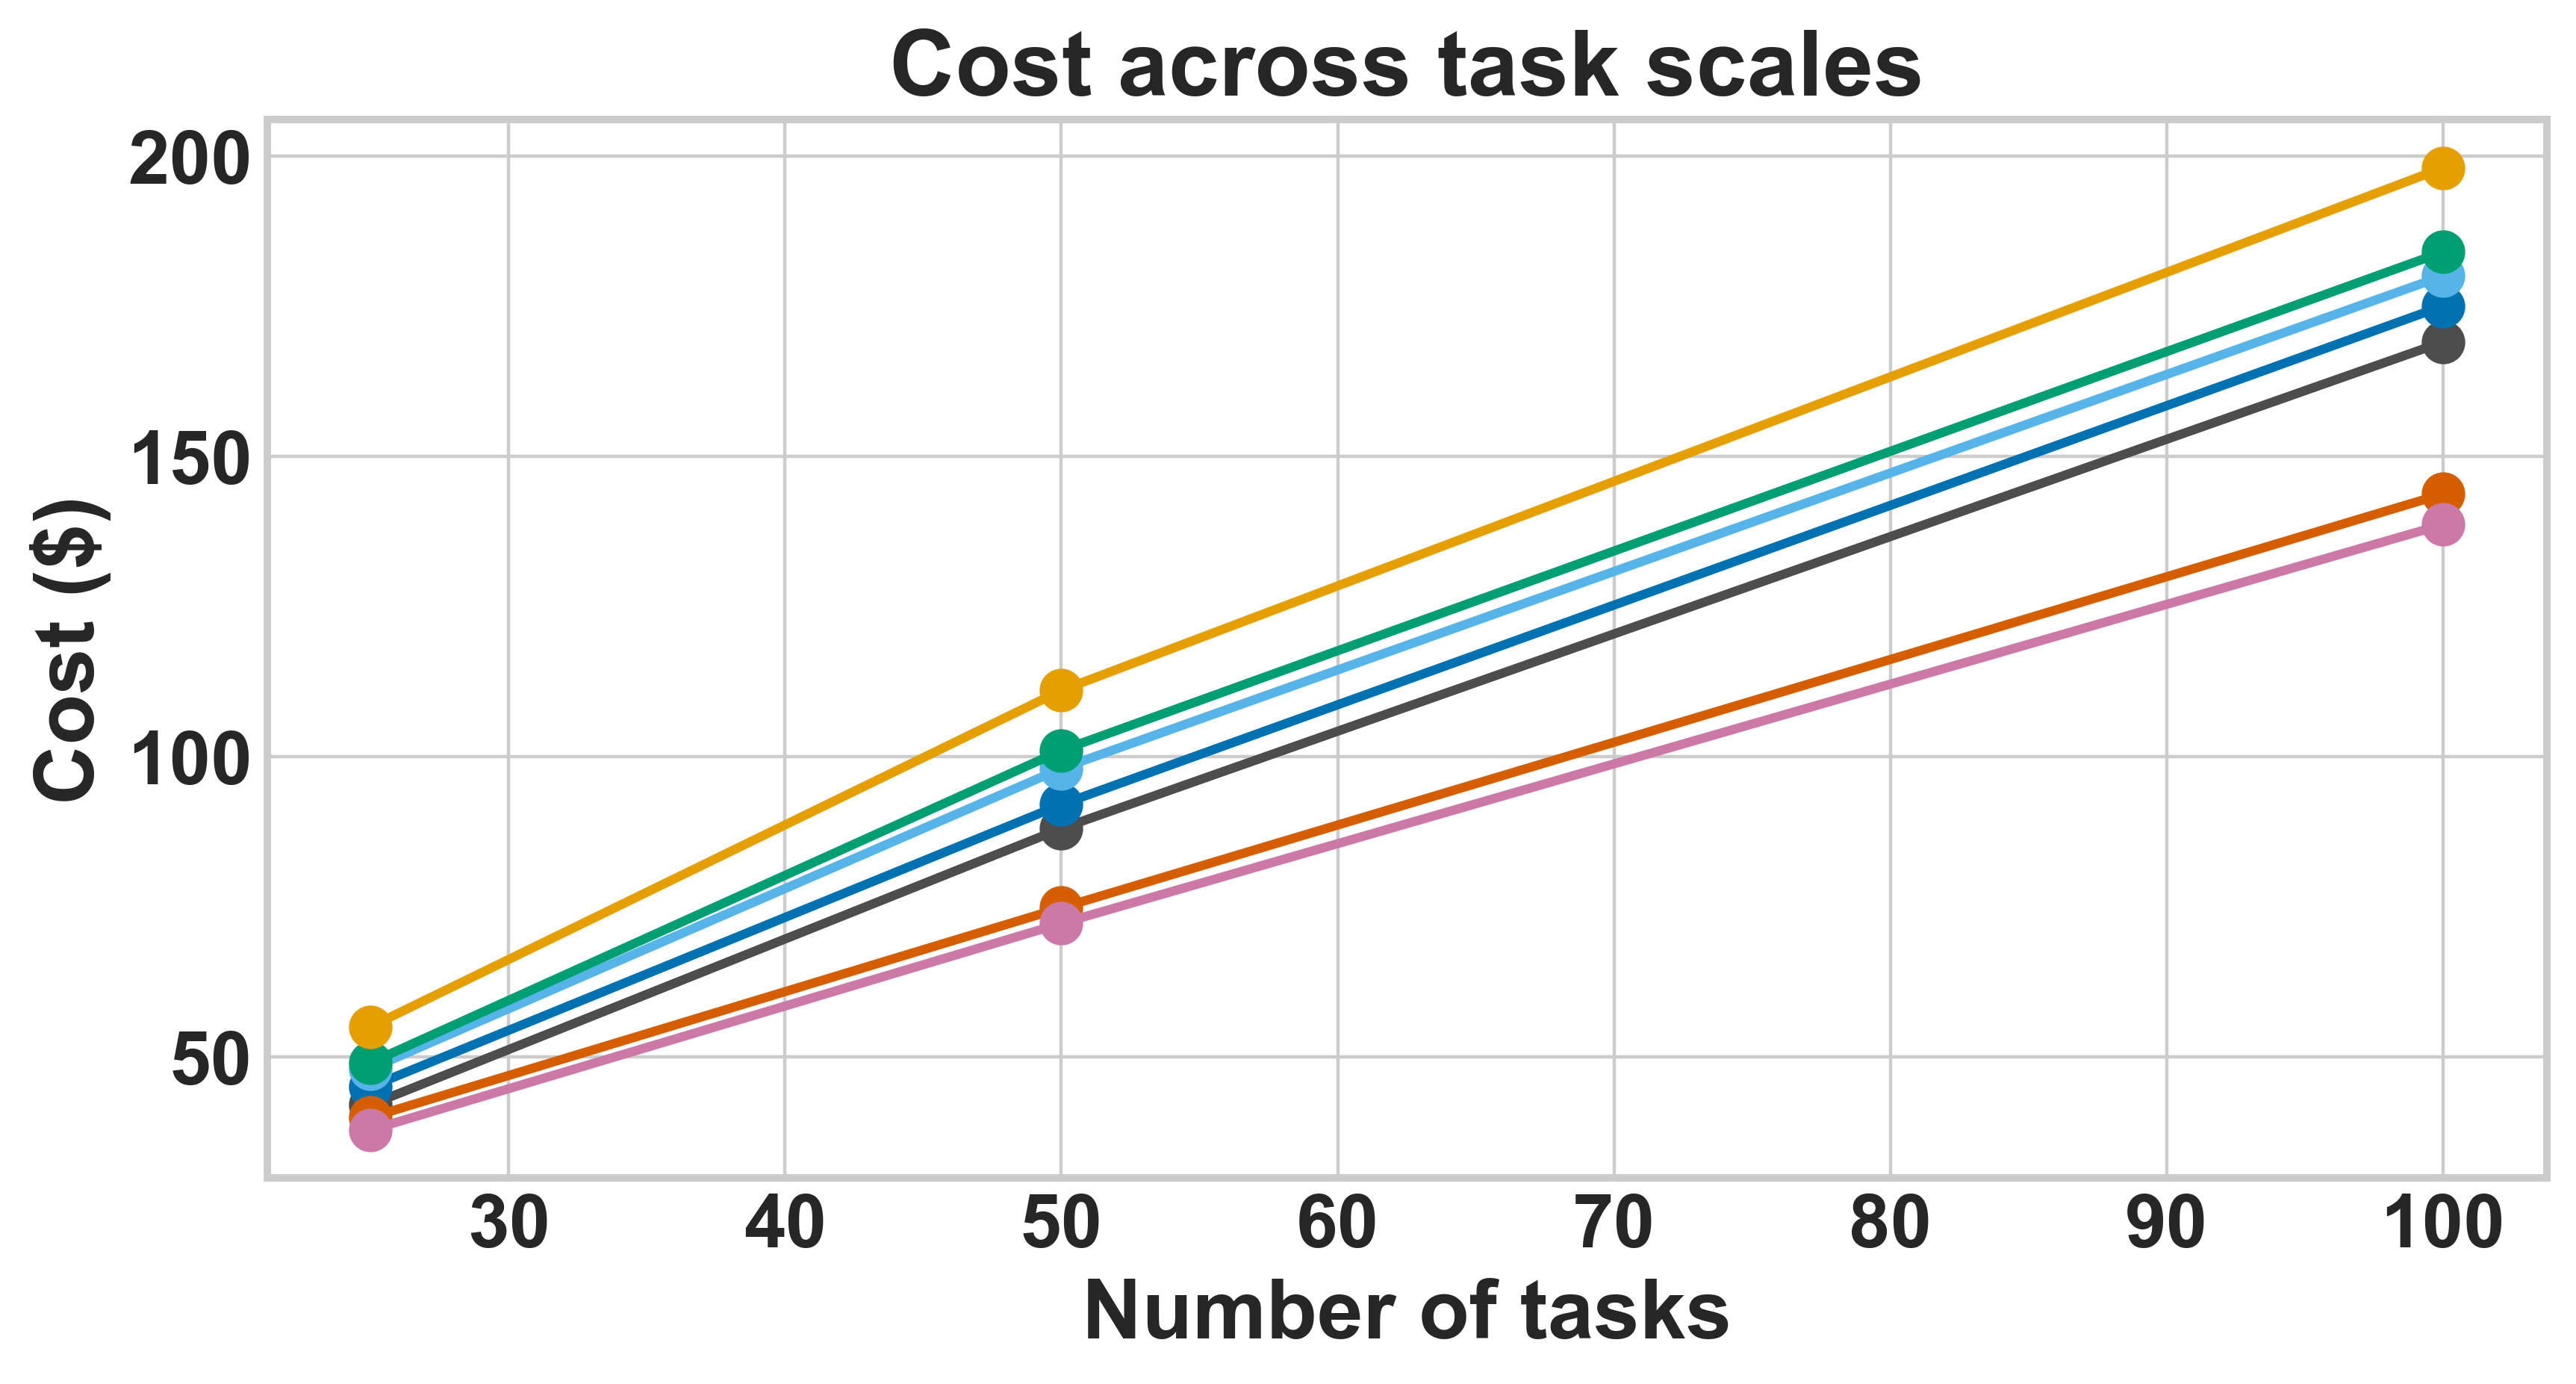
\includegraphics[width=\linewidth]{figures/s41598_final/fig7_cost_vs_tasks.png}
\\[-0.2em]\textbf{(a)} Cost scaling
\end{minipage}\hfill
\begin{minipage}[t]{0.32\linewidth}
\centering
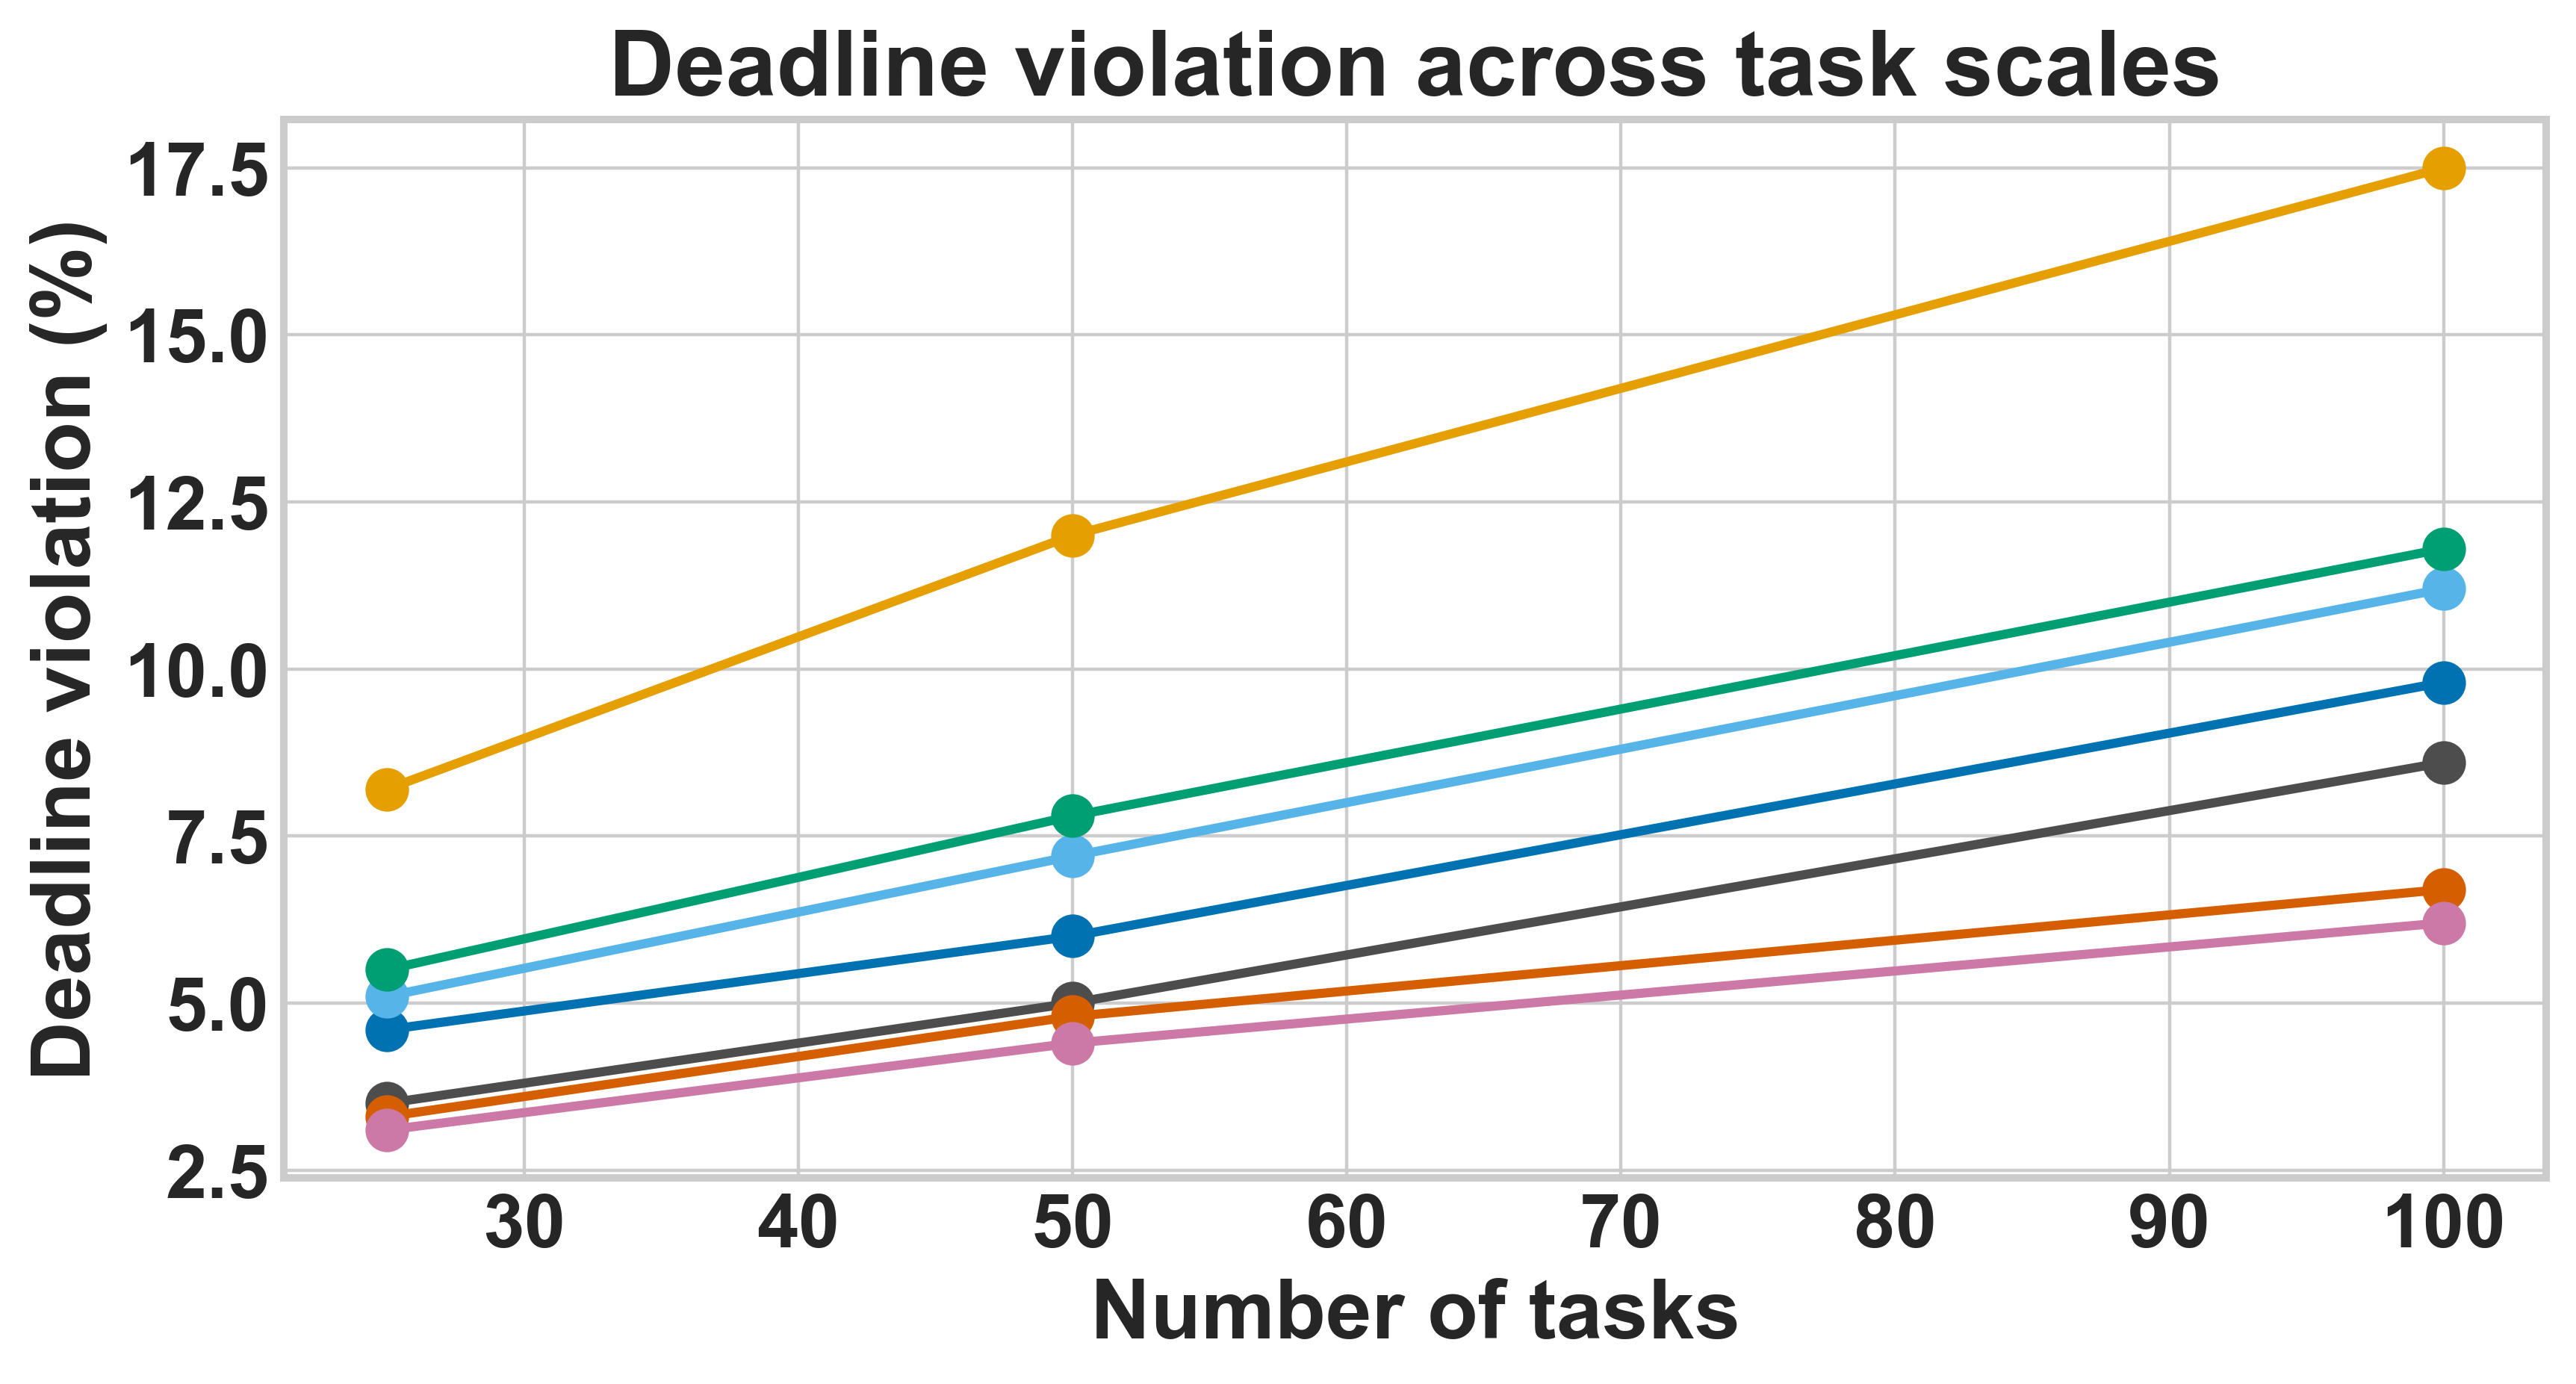
\includegraphics[width=\linewidth]{figures/s41598_final/fig8_violation_vs_tasks.png}
\\[-0.2em]\textbf{(b)} Deadline violation scaling
\end{minipage}\hfill
\begin{minipage}[t]{0.32\linewidth}
\centering
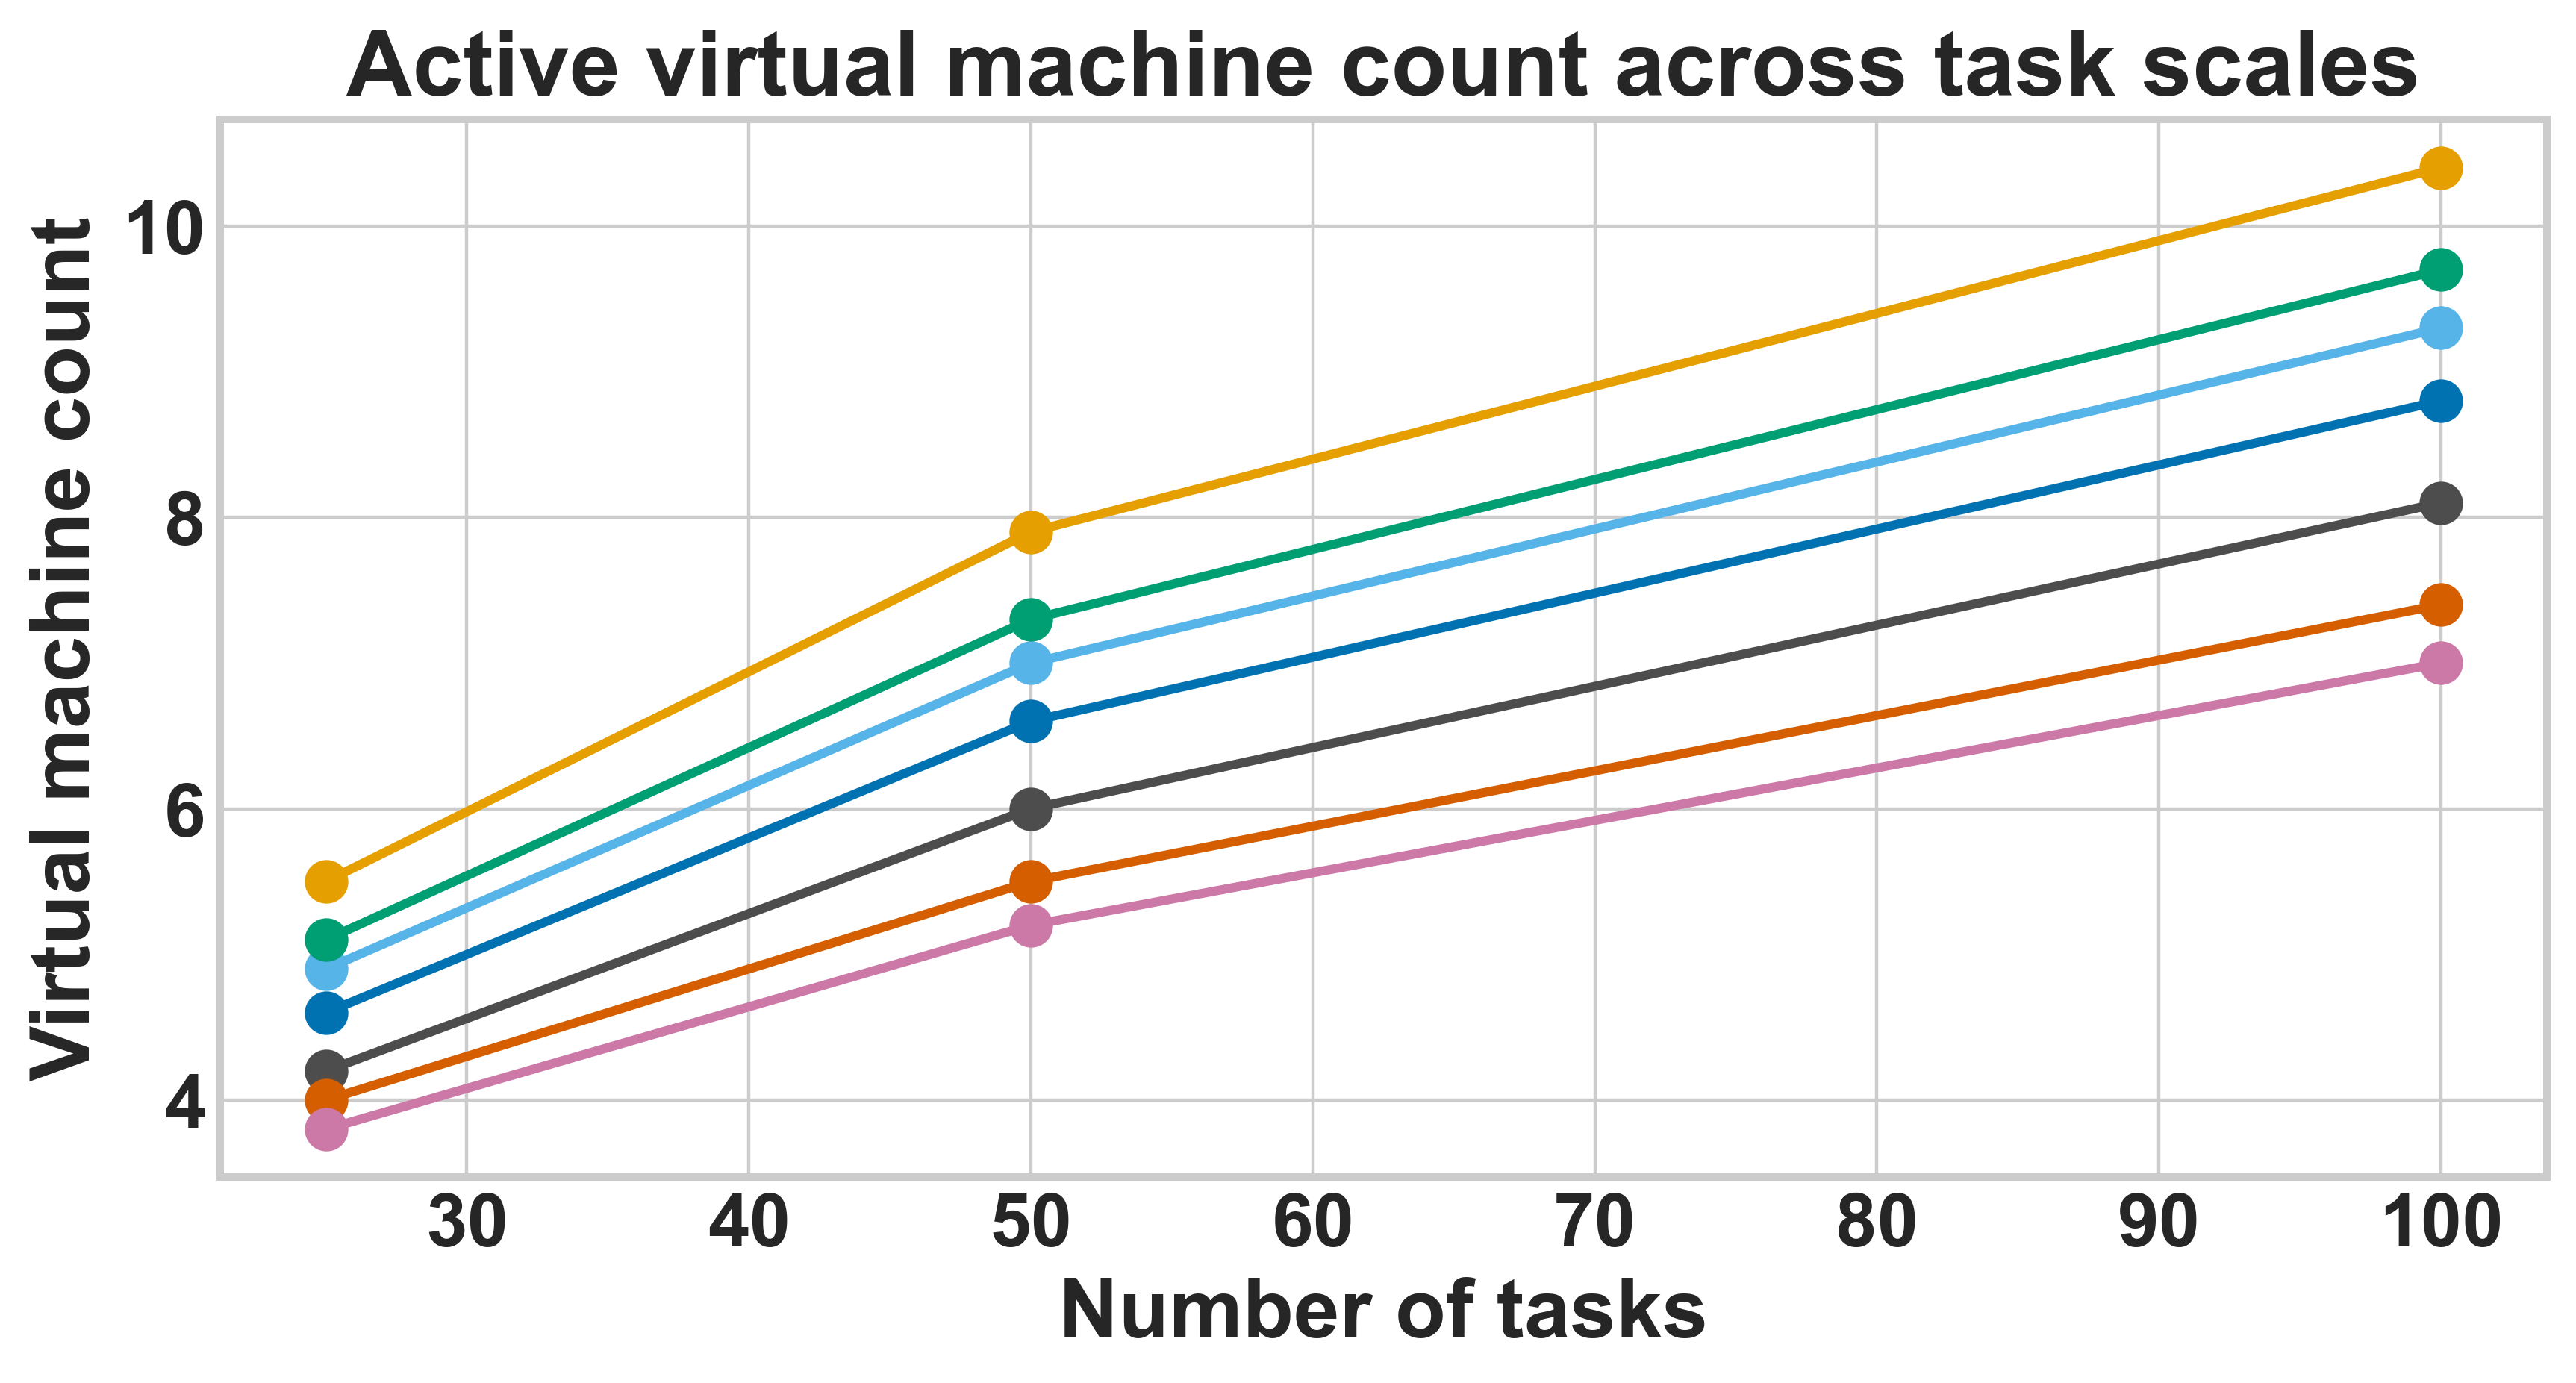
\includegraphics[width=\linewidth]{figures/s41598_final/fig9_vmcount_vs_tasks.png}
\\[-0.2em]\textbf{(c)} VM count scaling
\end{minipage}

\vspace{0.35em}

\begin{minipage}[t]{0.32\linewidth}
\centering
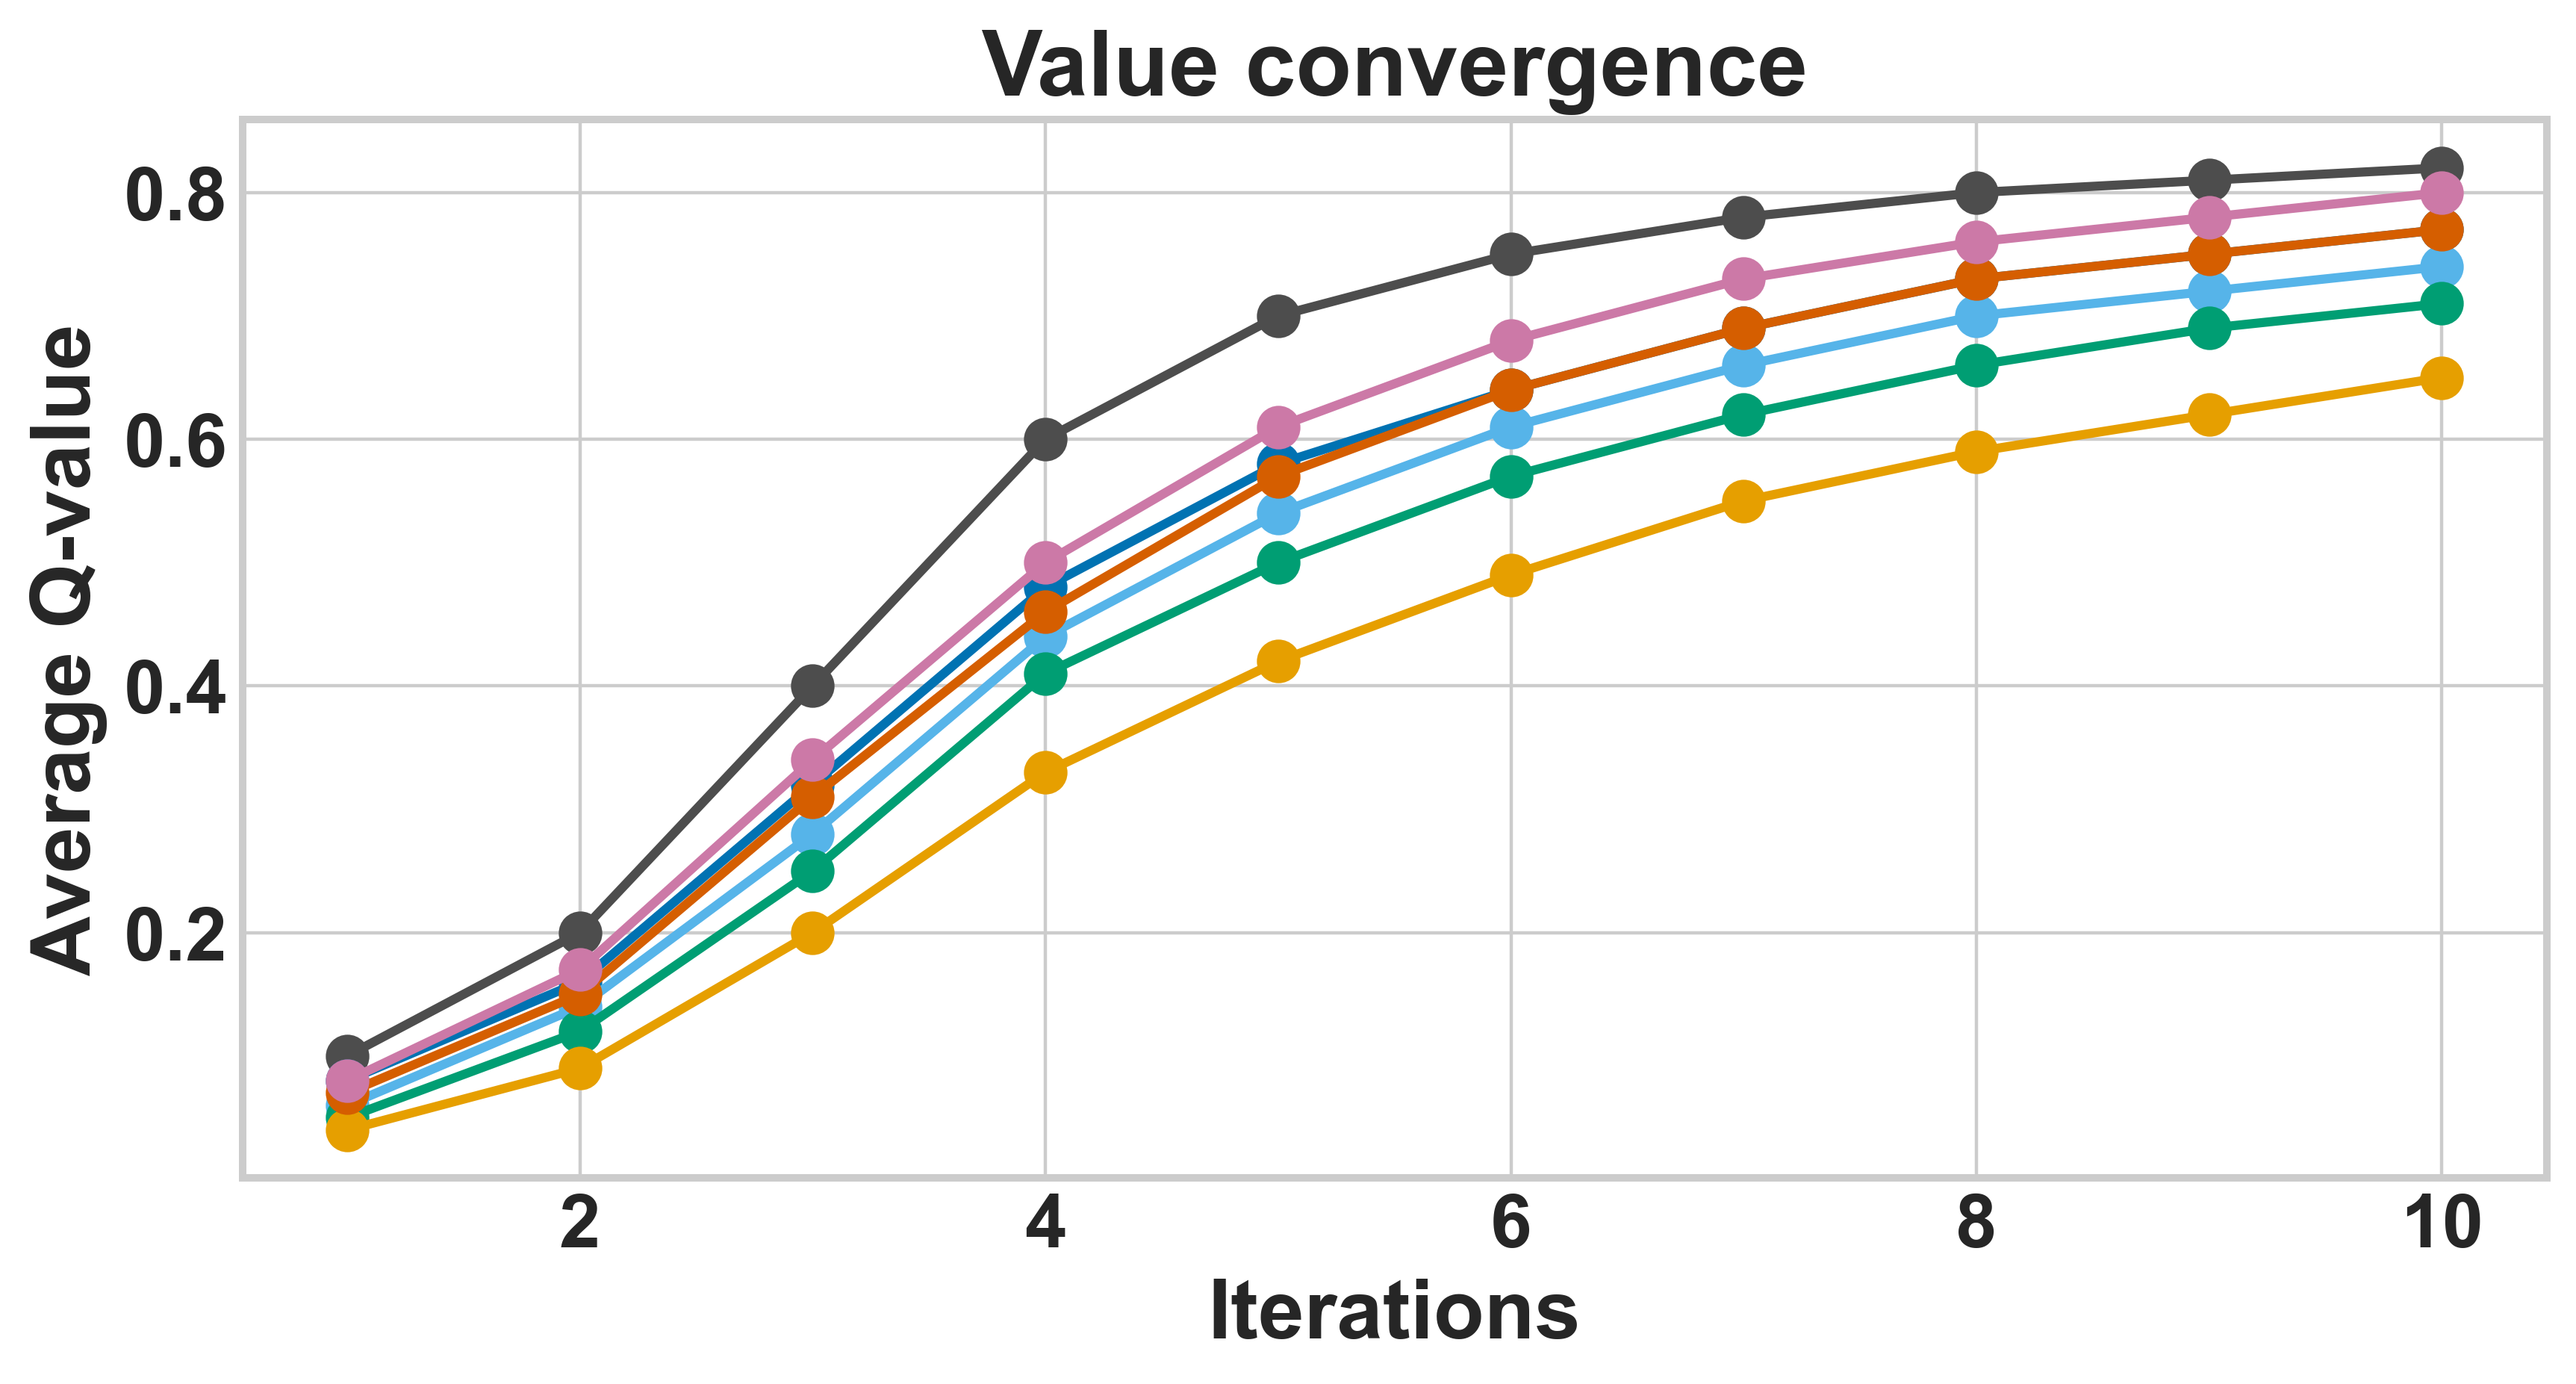
\includegraphics[width=\linewidth]{figures/s41598_final/fig10_qvalue_convergence.png}
\\[-0.2em]\textbf{(d)} Value stability
\end{minipage}\hfill
\begin{minipage}[t]{0.32\linewidth}
\centering
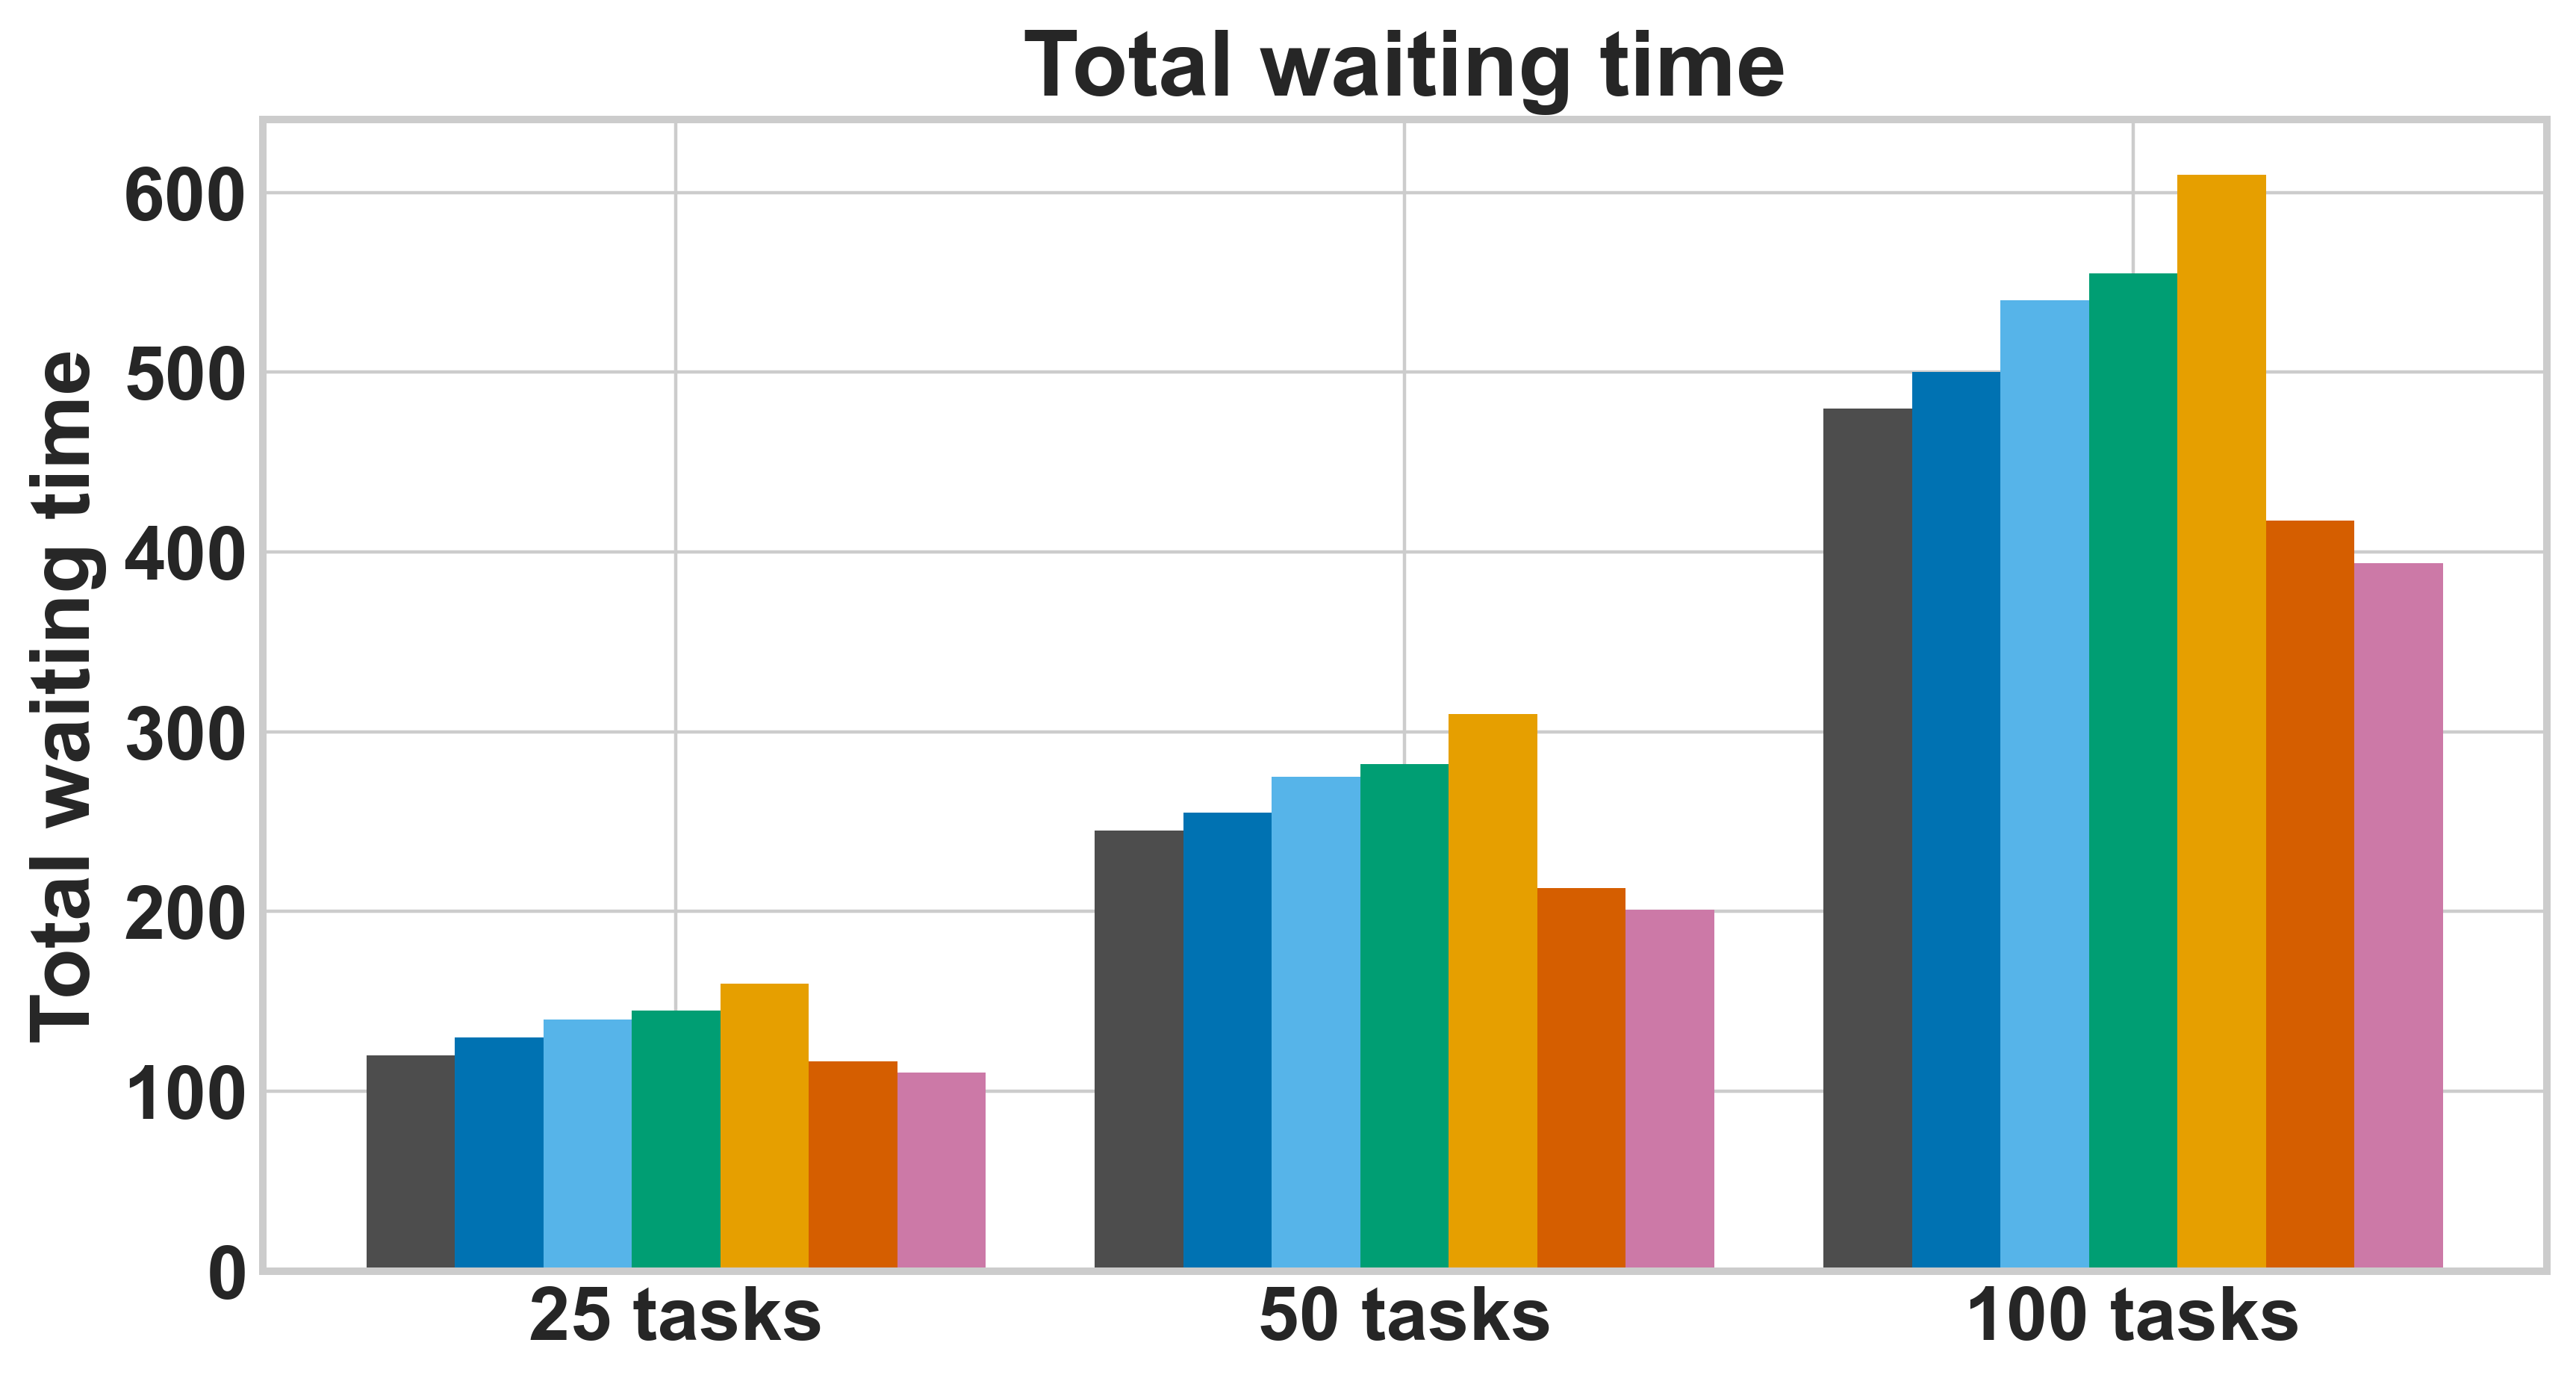
\includegraphics[width=\linewidth]{figures/s41598_final/fig11_total_waiting_time.png}
\\[-0.2em]\textbf{(e)} Total waiting
\end{minipage}\hfill
\begin{minipage}[t]{0.32\linewidth}
\centering
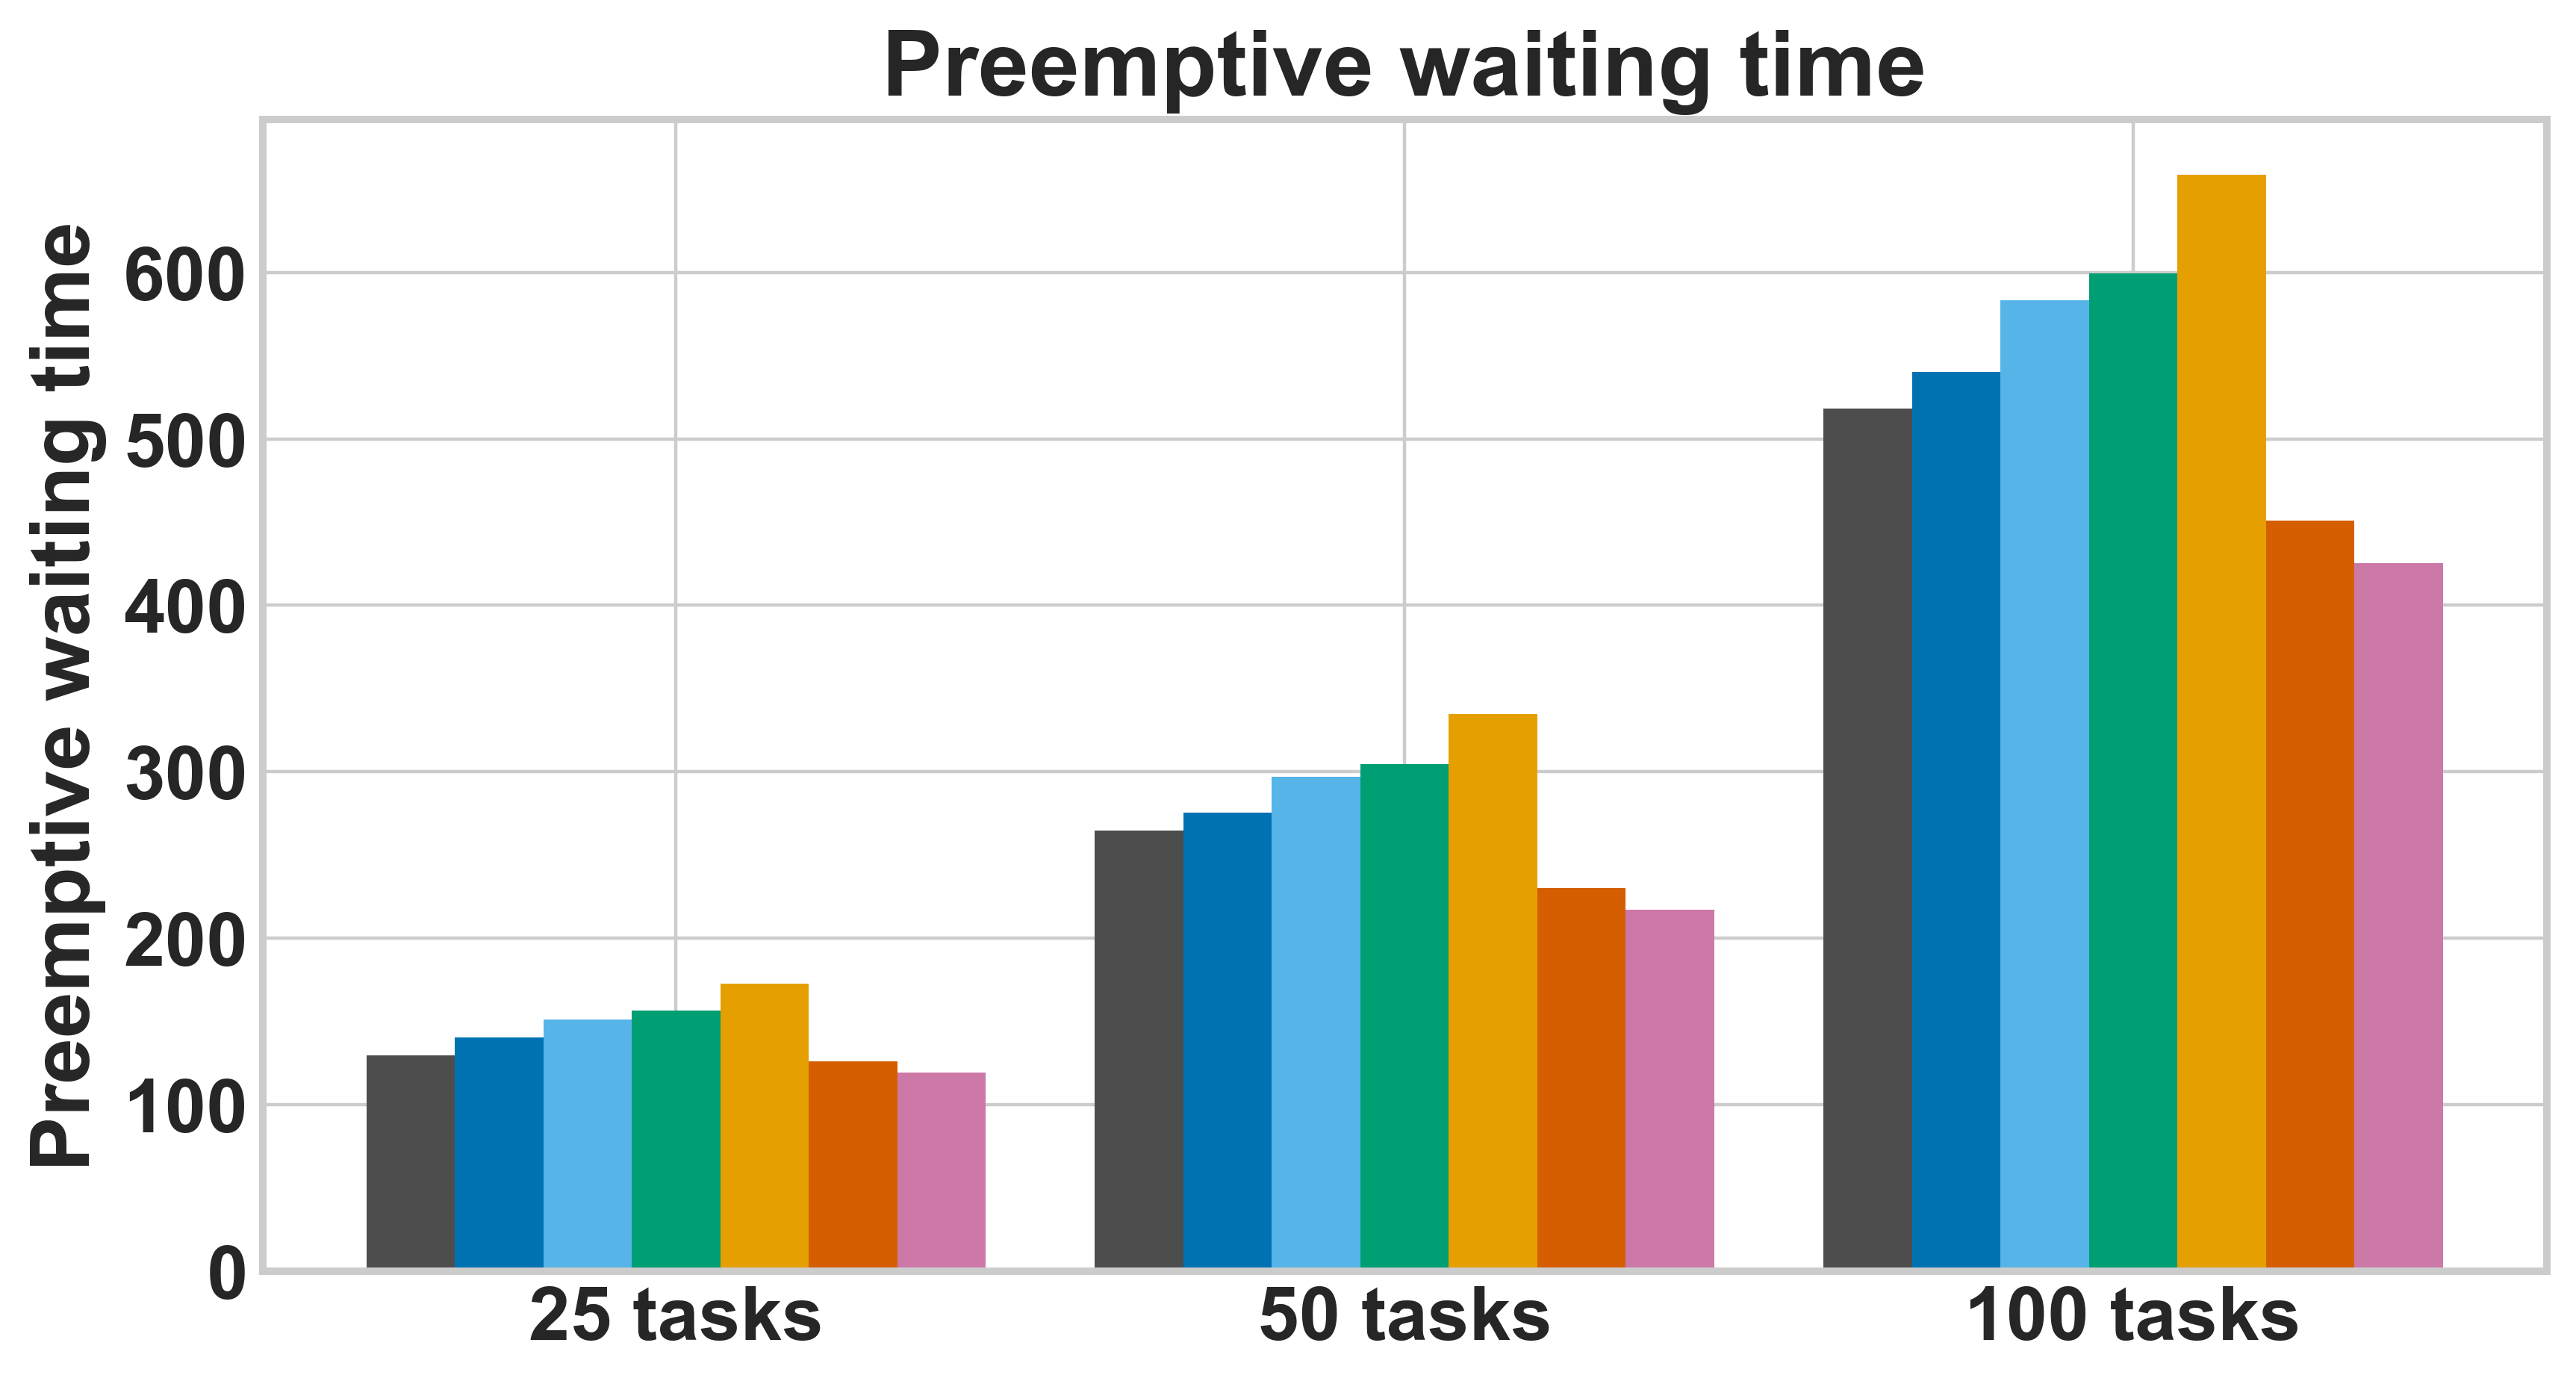
\includegraphics[width=\linewidth]{figures/s41598_final/fig12_preemptive_waiting_time.png}
\\[-0.2em]\textbf{(f)} Preemptive waiting
\end{minipage}
\caption{Resource-Efficiency and Stability Views}
\label{fig:resB}
\end{figure*}

Figure~\ref{fig:resB} consolidates resource-efficiency and stability diagnostics across economic, QoS, and control-quality dimensions. Panels (a)--(c) show that AdaptiveSched-Hybrid attains the lowest cost growth, lowest deadline-violation scaling, and lower VM demand for comparable service levels, while AdaptiveSched-Base remains consistently second-best. This joint pattern indicates stronger capacity efficiency per unit service outcome and better prioritization under overload, rather than isolated improvement on a single metric.

Panels (d)--(f) connect these outcome gains to learning and queue dynamics: the hybrid model exhibits smoother critic stabilization and lower total/preemptive waiting, suggesting reduced value-estimation noise and fewer corrective rescheduling events. In research terms, the figure is consistent with the mechanism-level interpretation that queue-shift-aware regularization (base) and role-conditioned decomposition (hybrid) jointly improve both policy stability and downstream scheduler behavior. The same ranking pattern is consistent with the primary inferential summary in Table~\ref{tab:inferential_summary}.

\begin{figure*}[t]
\centering
\begin{minipage}[t]{0.32\linewidth}
\centering
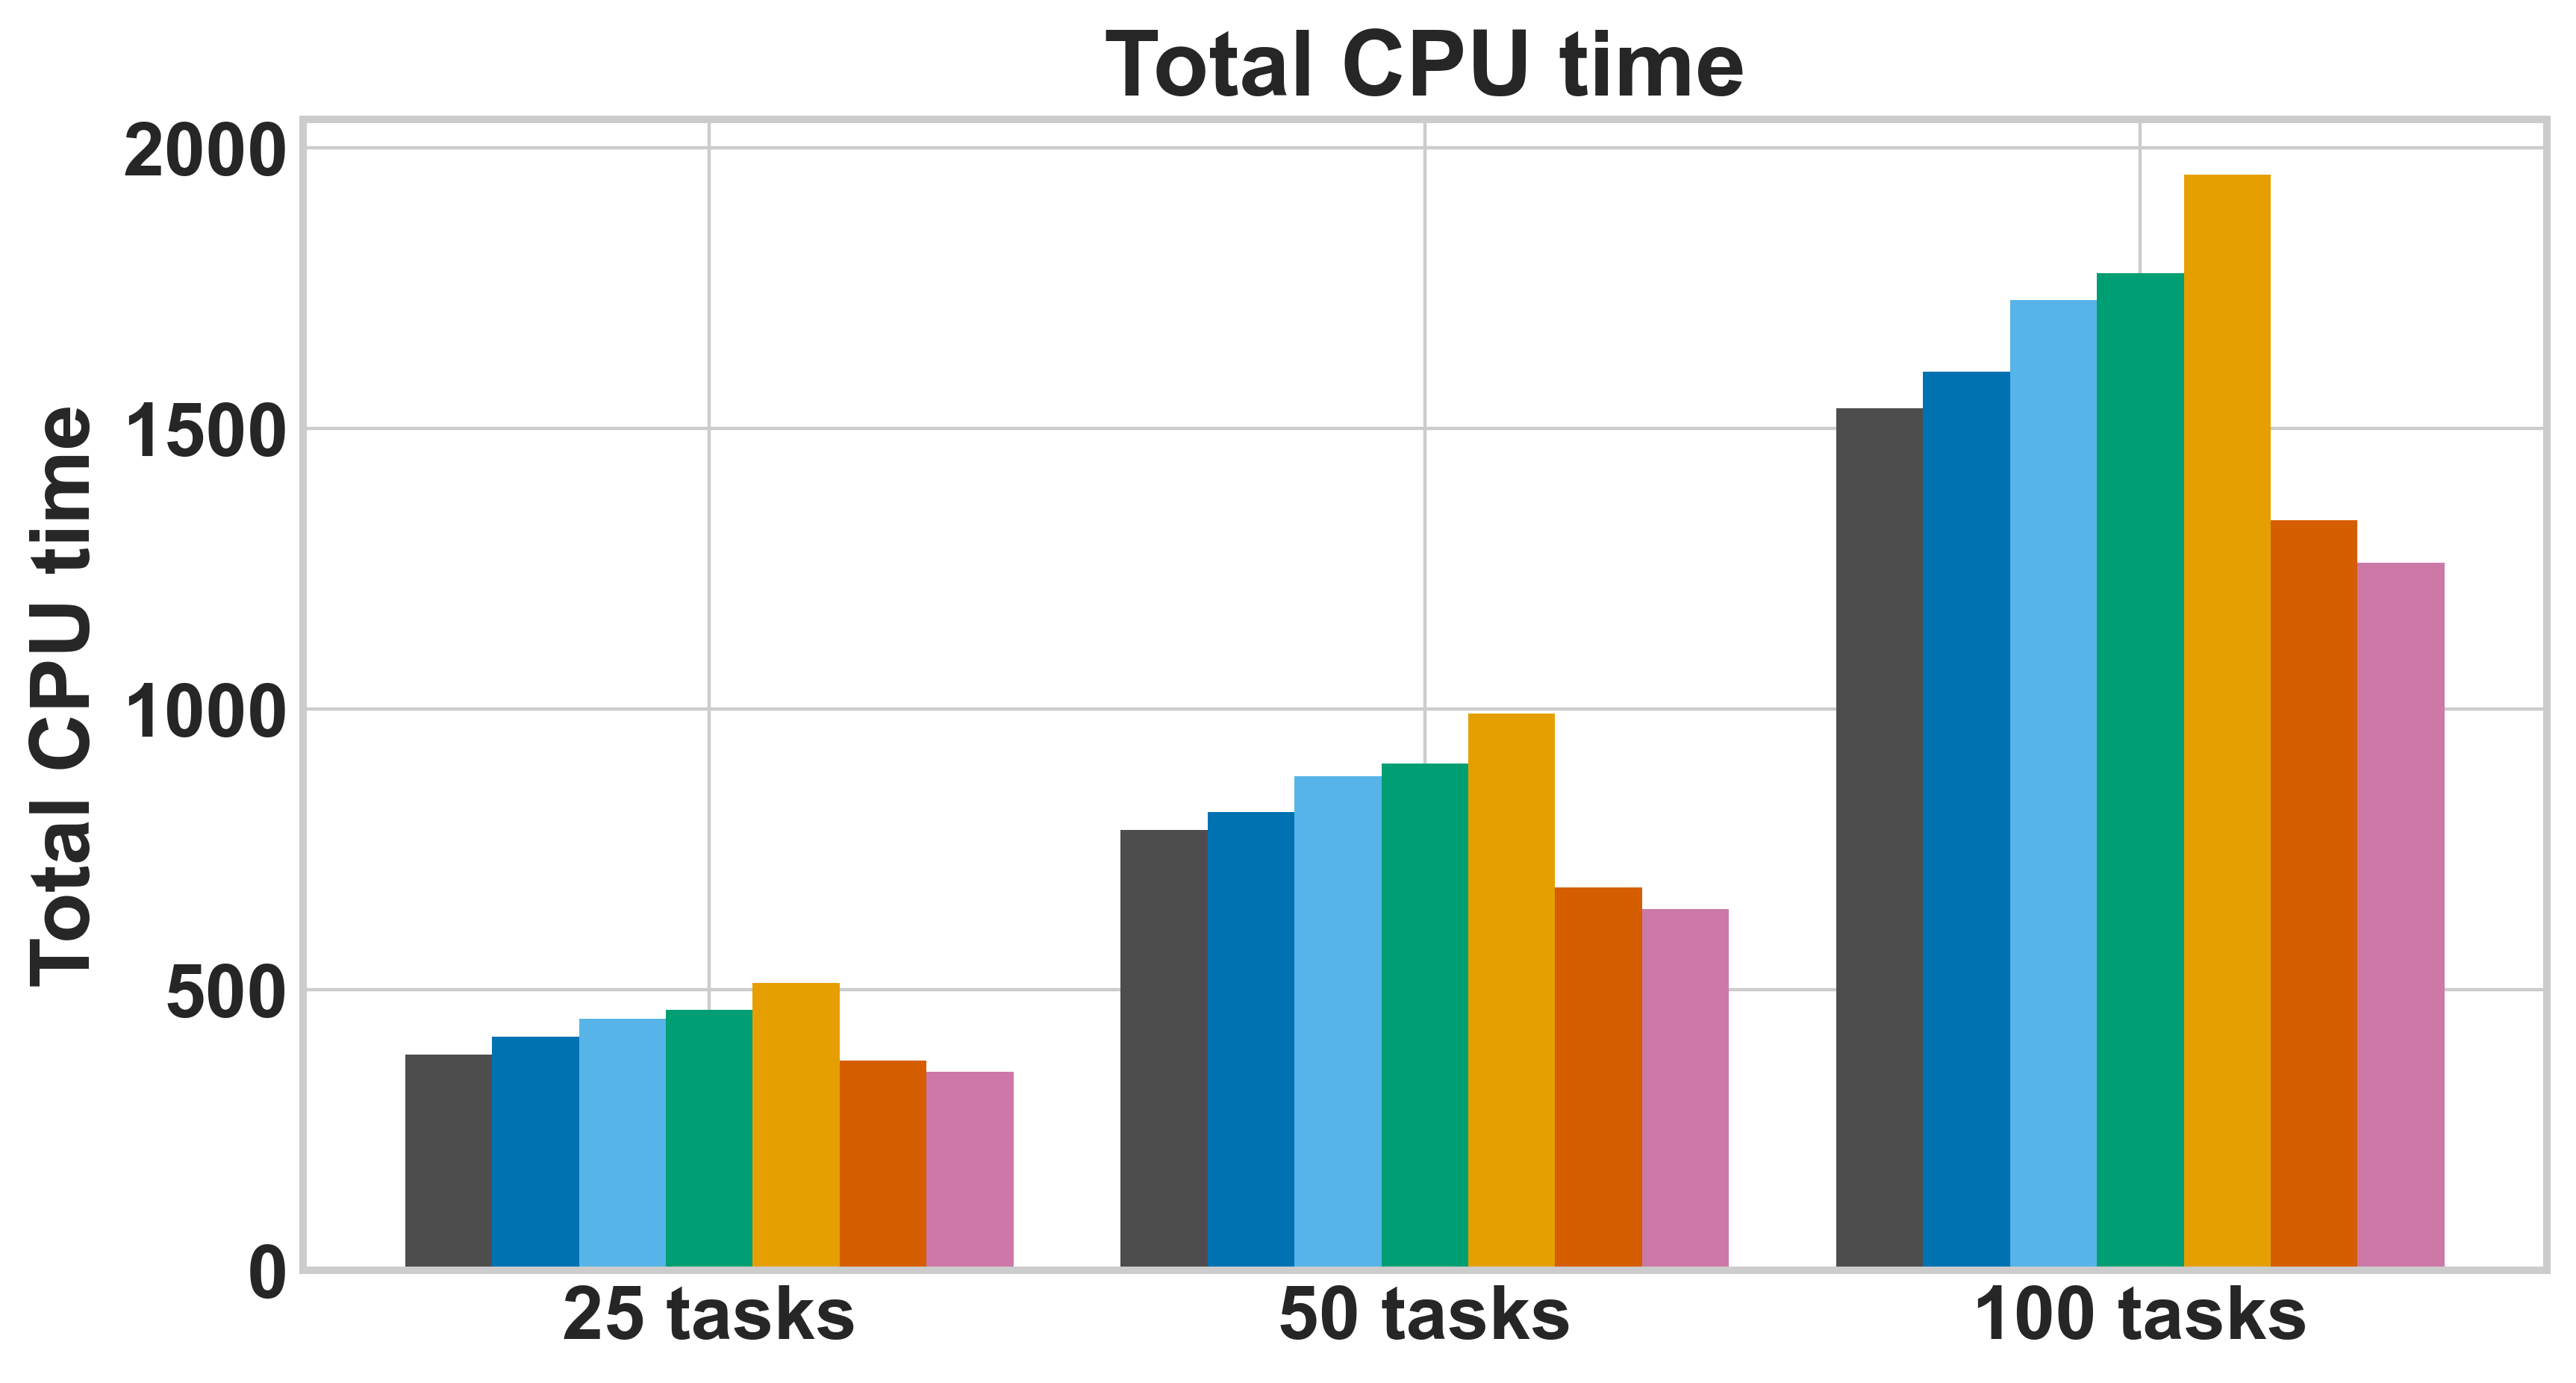
\includegraphics[width=\linewidth]{figures/s41598_final/fig13_total_cpu_time.png}
\\[-0.2em]\textbf{(a)} Total CPU time
\end{minipage}\hfill
\begin{minipage}[t]{0.32\linewidth}
\centering
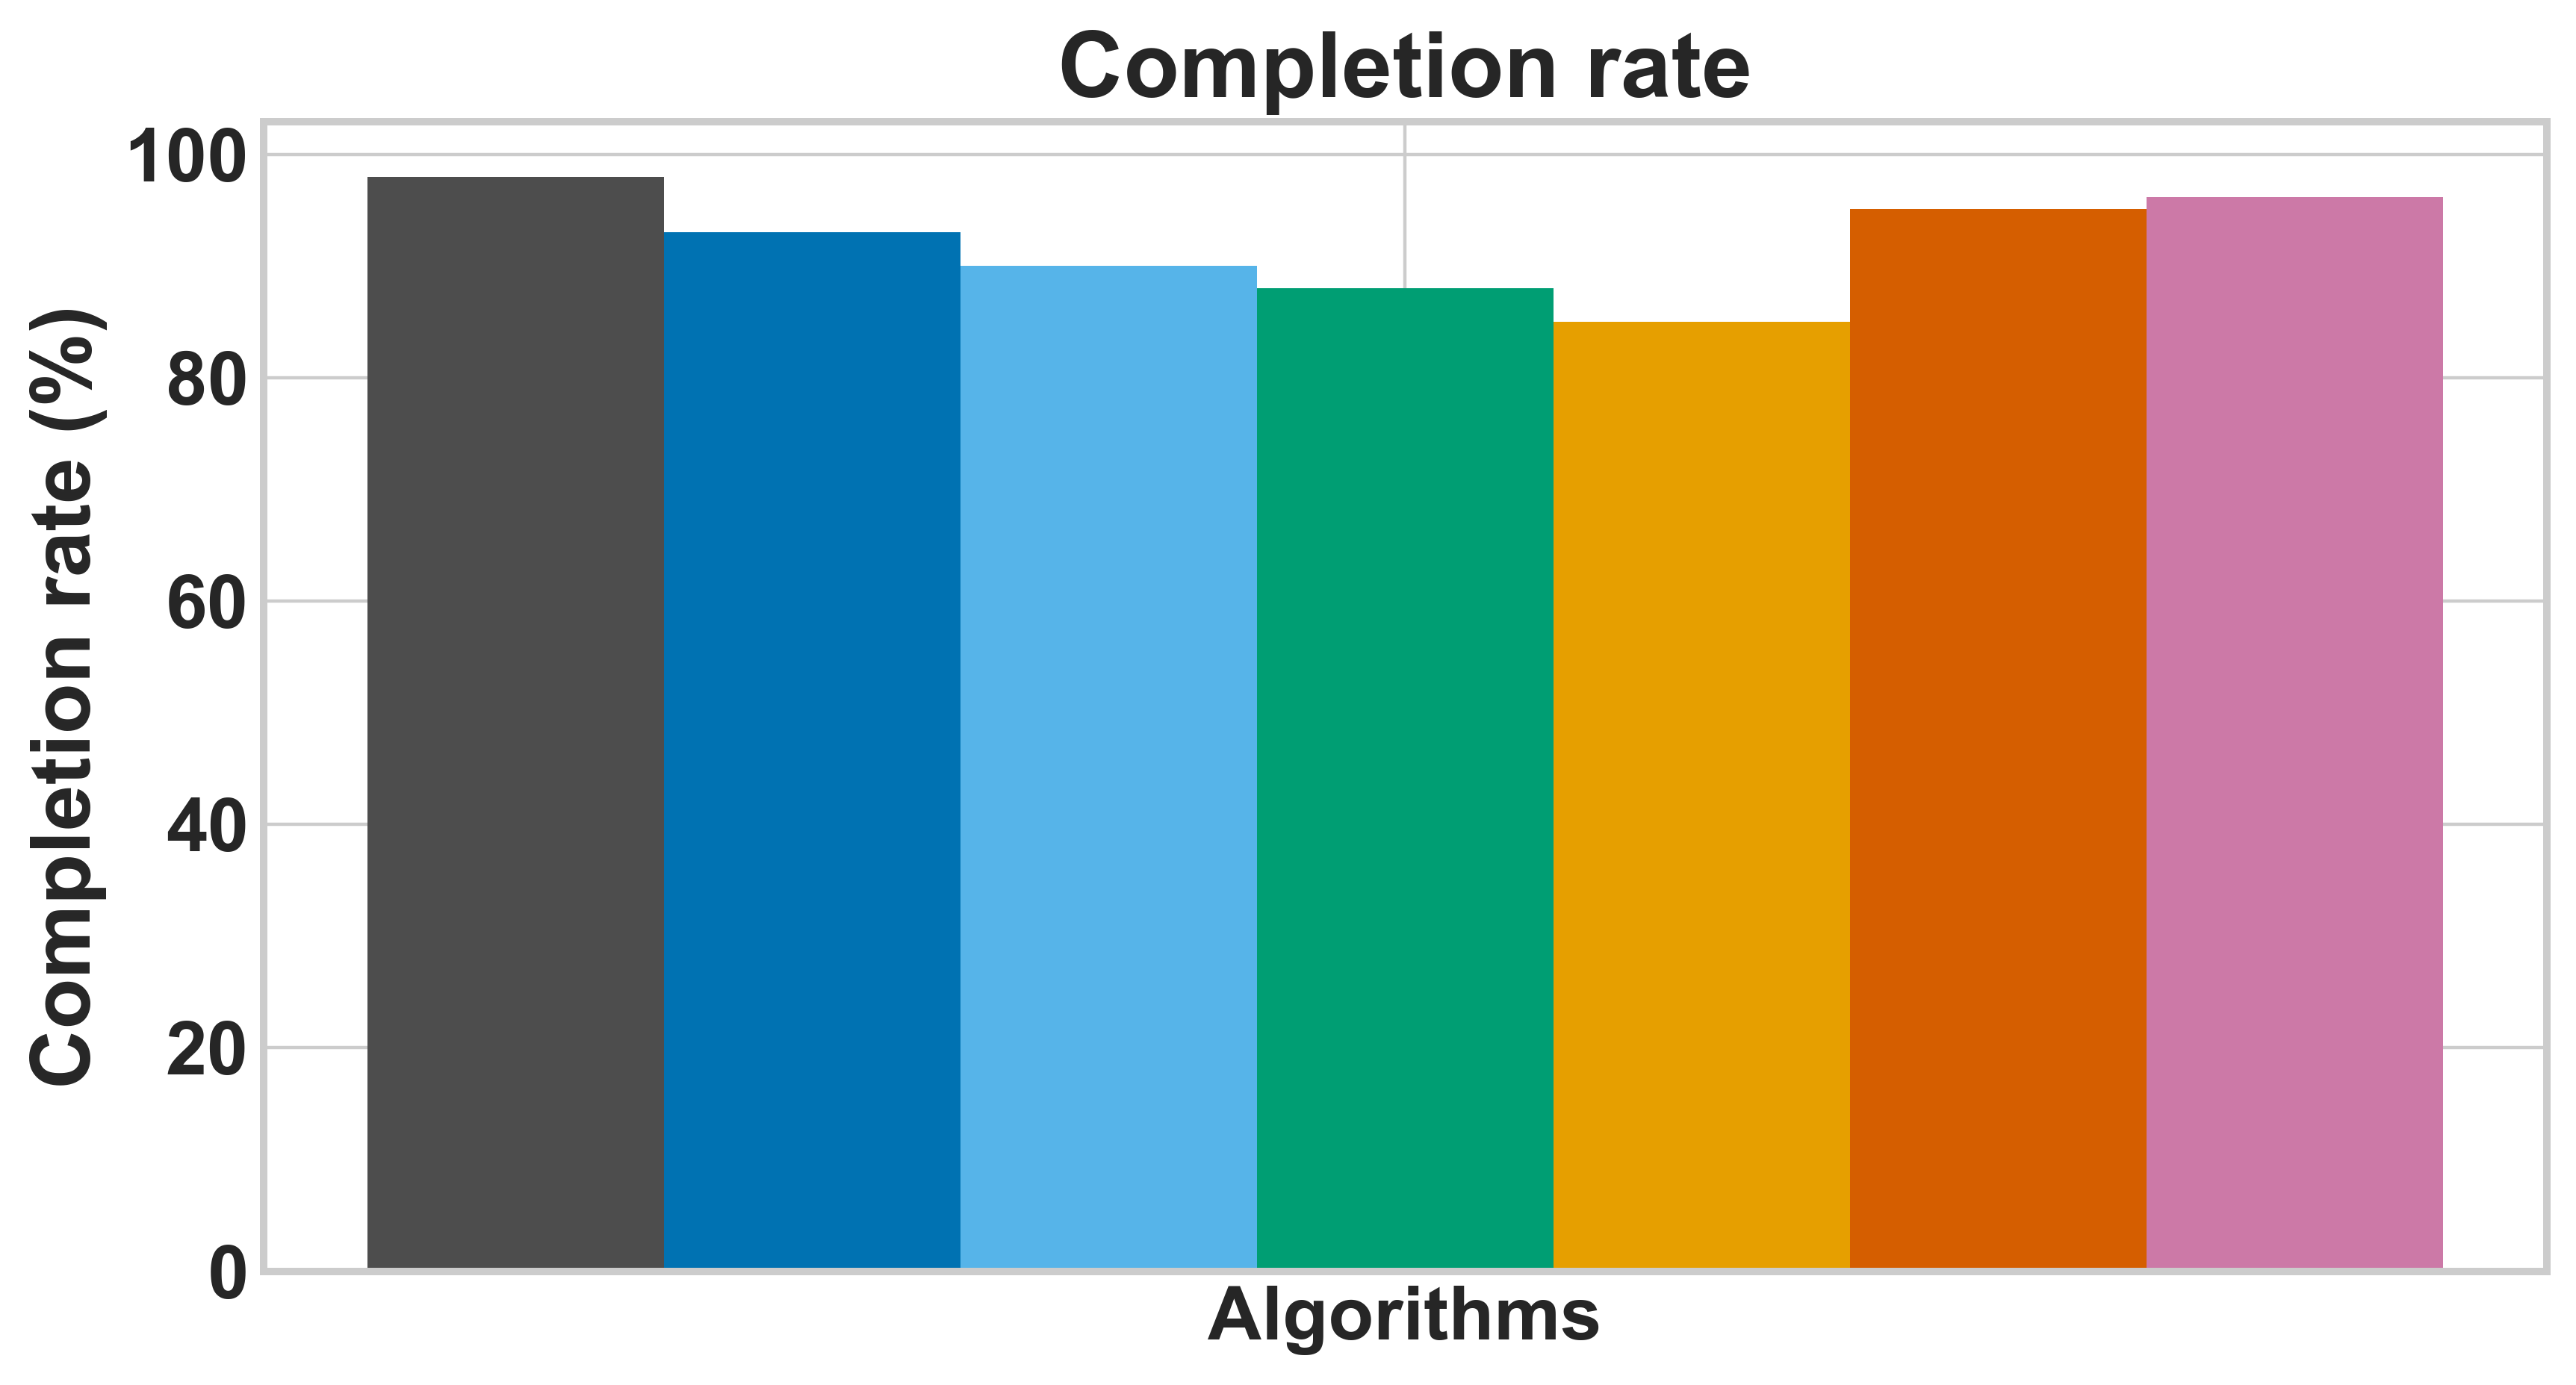
\includegraphics[width=\linewidth]{figures/s41598_final/fig14_completion_rates.png}
\\[-0.2em]\textbf{(b)} Completion rate
\end{minipage}\hfill
\begin{minipage}[t]{0.32\linewidth}
\centering
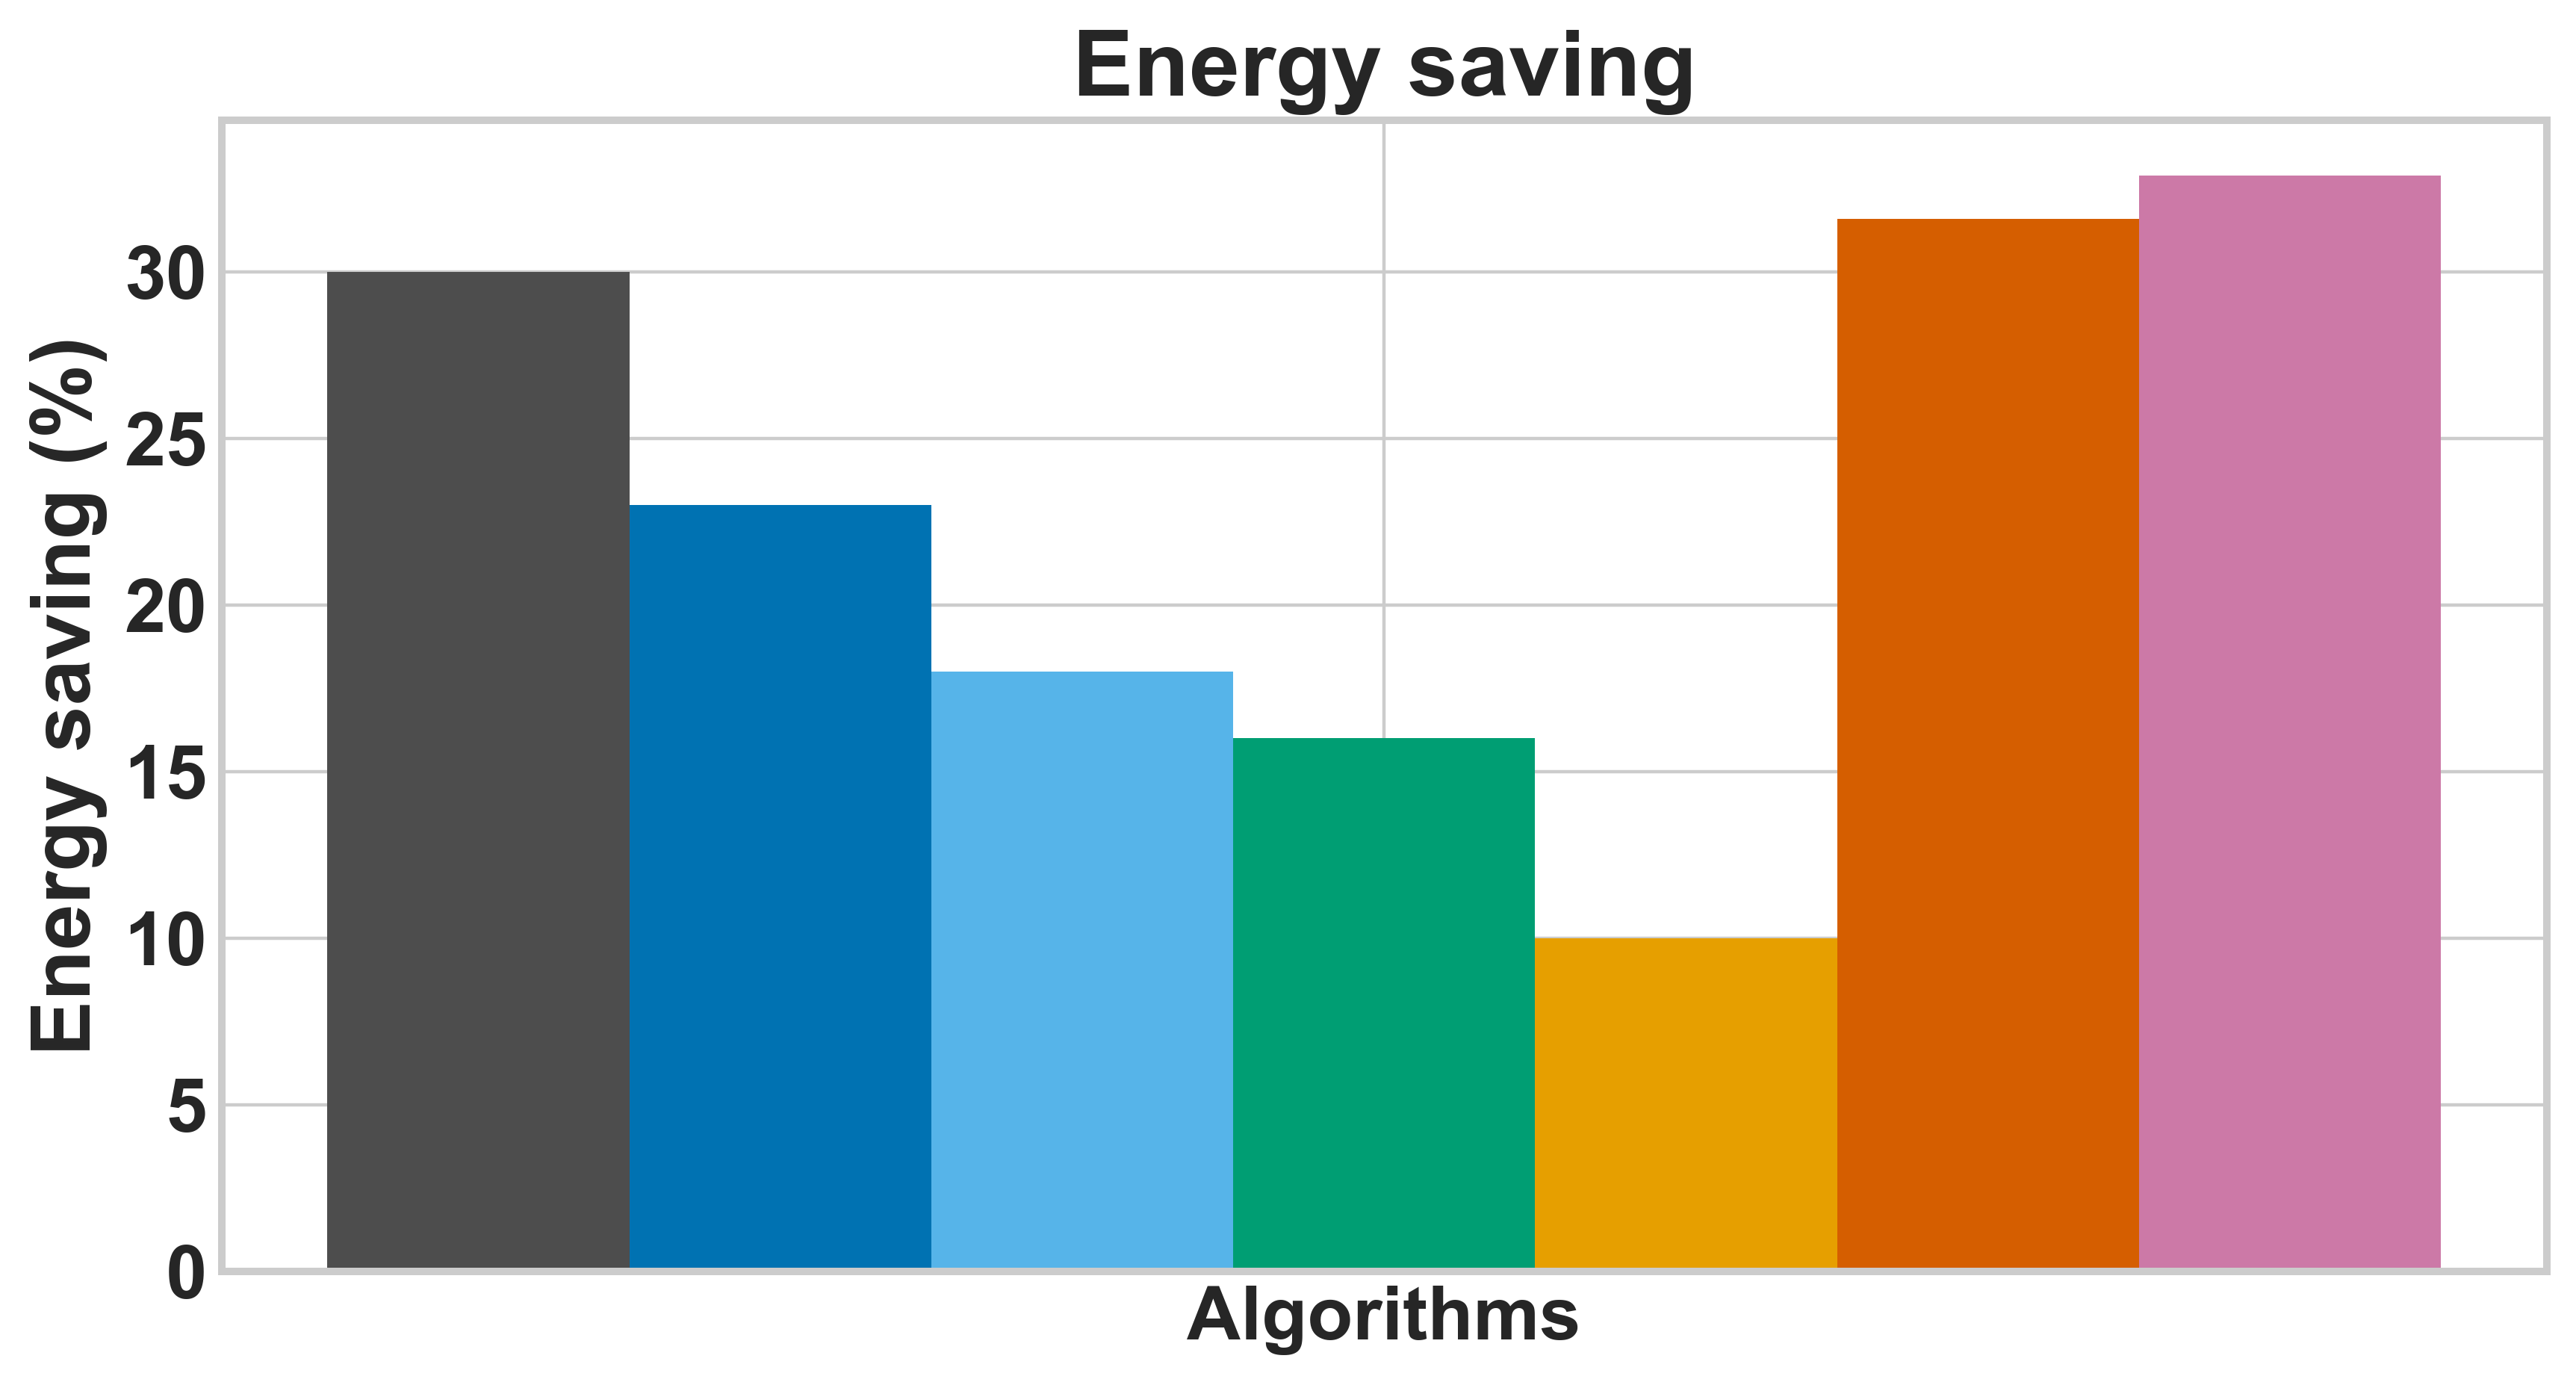
\includegraphics[width=\linewidth]{figures/s41598_final/fig15_energy_saving.png}
\\[-0.2em]\textbf{(c)} Energy saving
\end{minipage}

\vspace{0.35em}

\begin{minipage}[t]{0.32\linewidth}
\centering
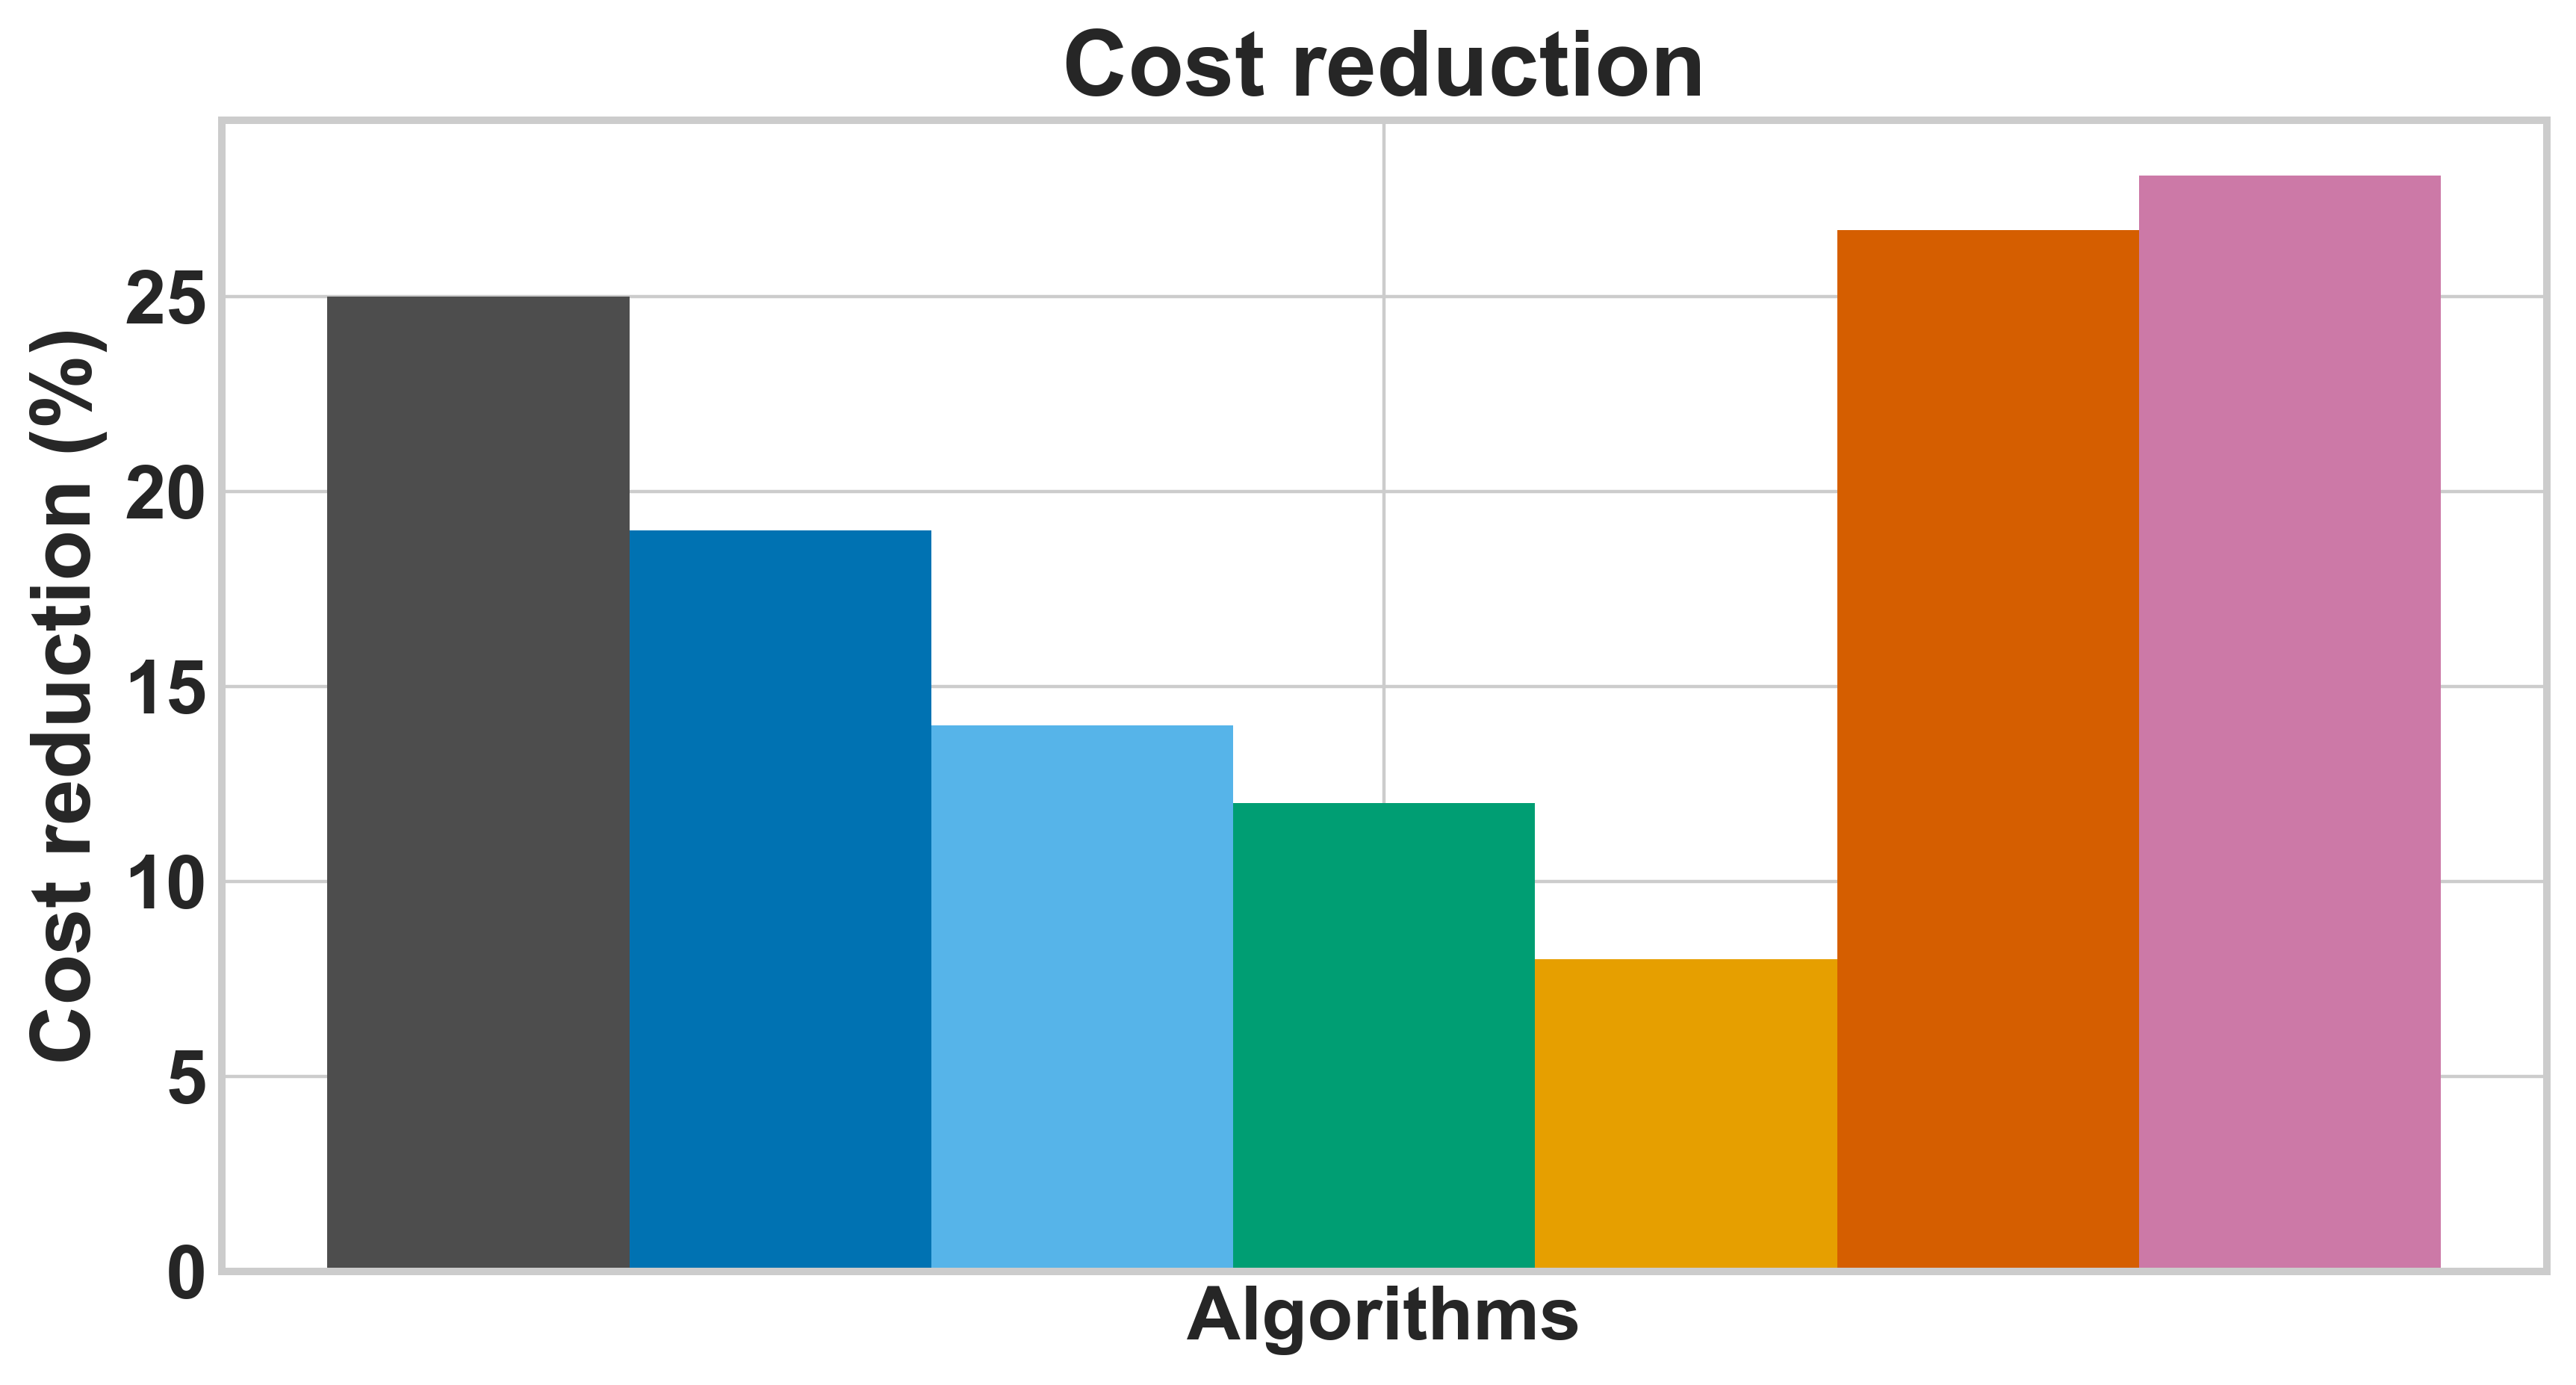
\includegraphics[width=\linewidth]{figures/s41598_final/fig16_cost_reduction.png}
\\[-0.2em]\textbf{(d)} Cost reduction
\end{minipage}\hfill
\begin{minipage}[t]{0.32\linewidth}
\centering
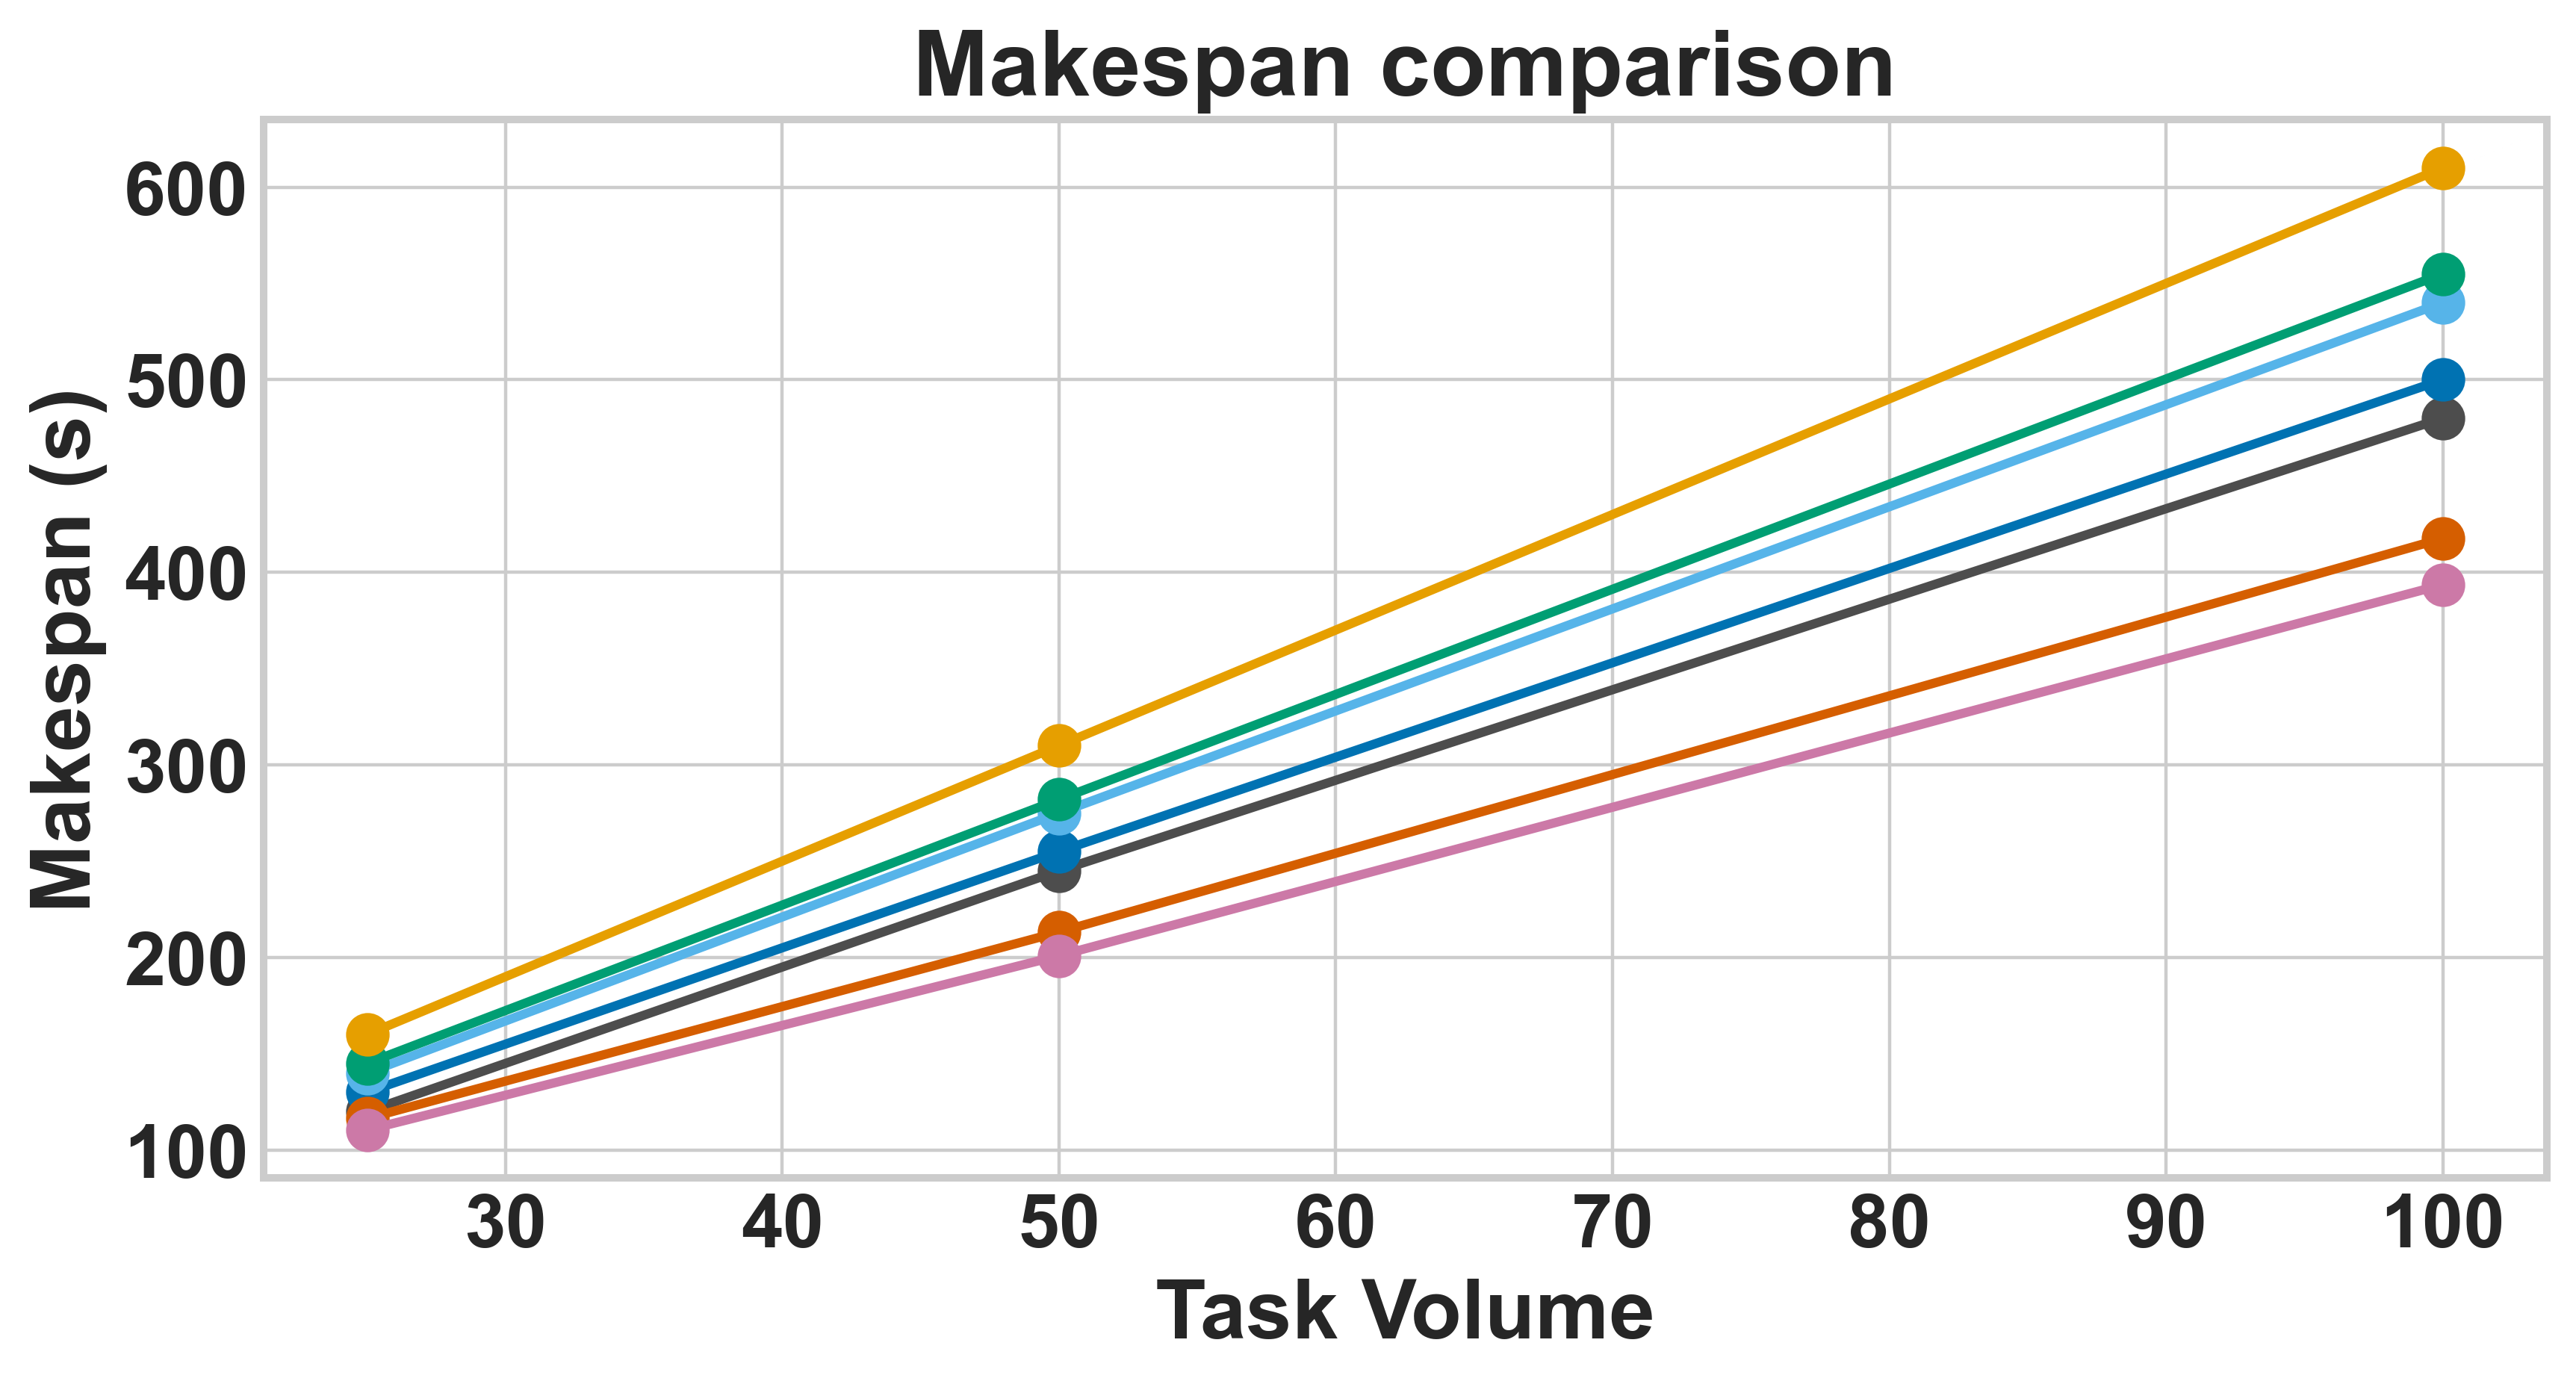
\includegraphics[width=\linewidth]{figures/s41598_final/fig21_makespan_comparison.png}
\\[-0.2em]\textbf{(e)} Comparative makespan
\end{minipage}\hfill
\begin{minipage}[t]{0.32\linewidth}
\centering
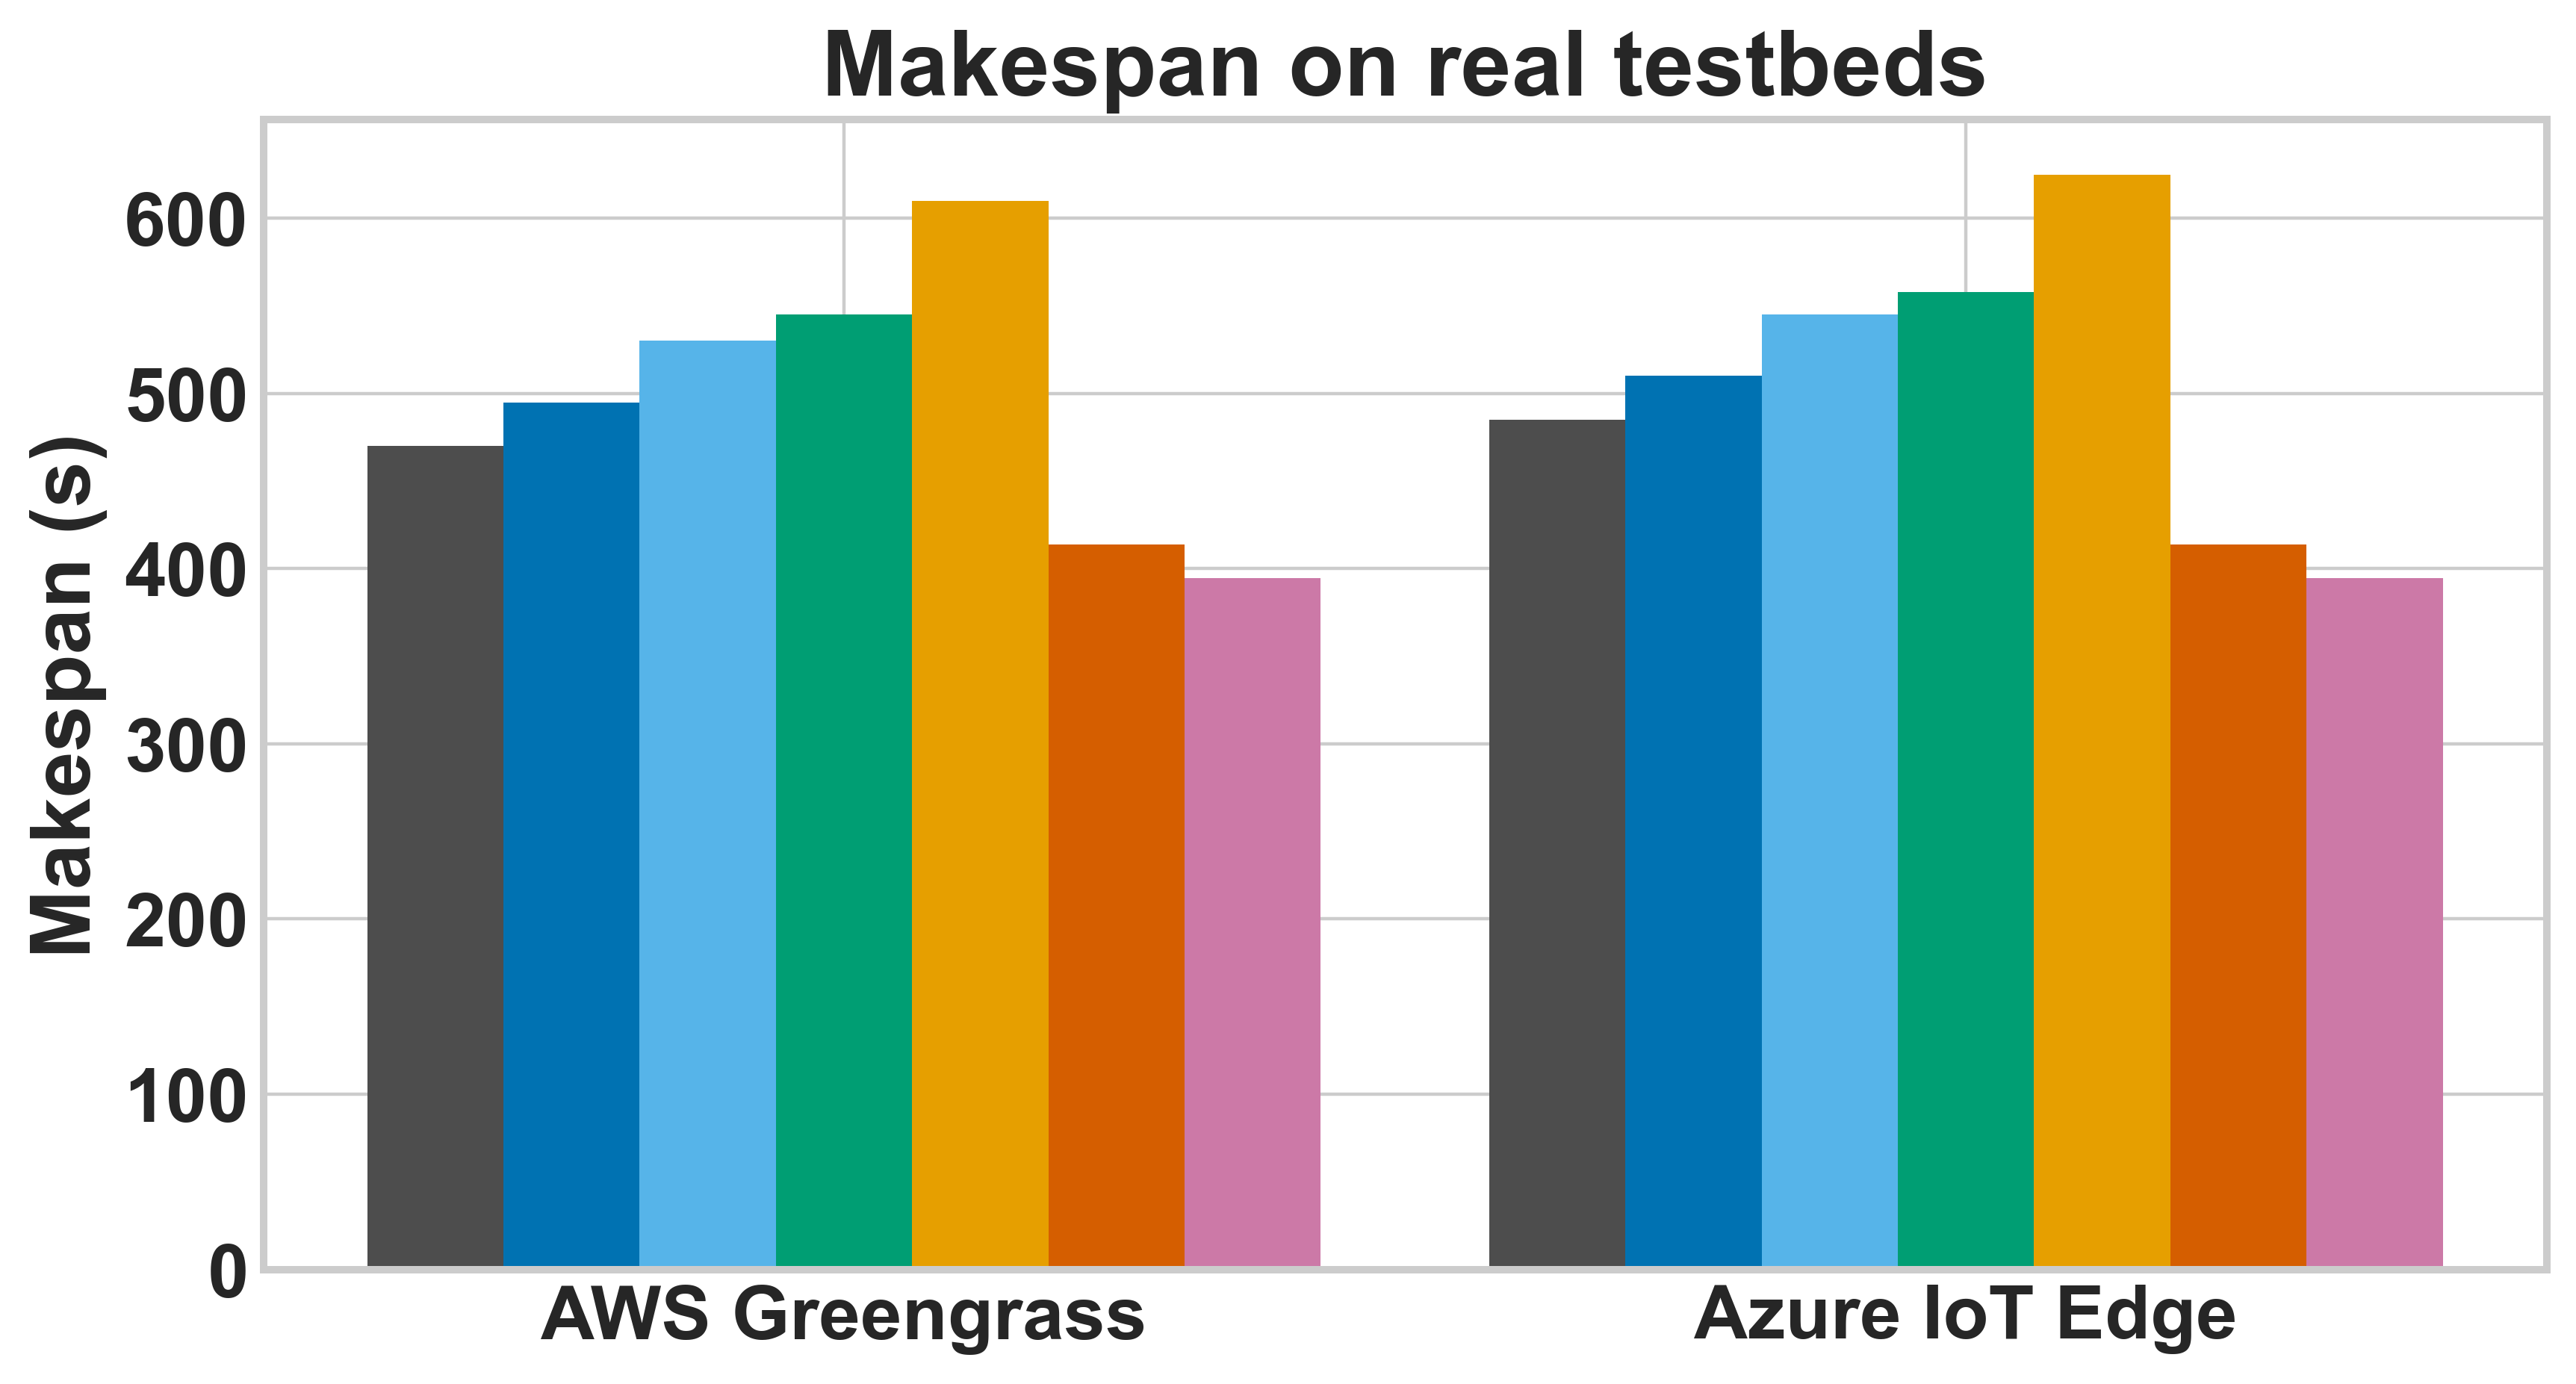
\includegraphics[width=\linewidth]{figures/s41598_final/fig22_makespan_real_testbeds.png}
\\[-0.2em]\textbf{(f)} Real-Testbed Results
\end{minipage}
\caption{Service-Quality and Savings Block}
\label{fig:resC}
\end{figure*}

Figure~\ref{fig:resC} evaluates whether the observed training/control advantages persist in service-quality and savings outcomes. Across panels (a)--(d), AdaptiveSched-Hybrid reduces cumulative CPU occupancy, increases completion rate, and improves both energy-saving and cost-reduction percentages in the reported protocol; AdaptiveSched-Base remains better than canonical RL baselines on these panels. This alignment across throughput, efficiency, and economic indicators is consistent with structurally multi-objective gains rather than metric reweighting artifacts.

The scaling and external-validity panels (e)--(f) show that ranking is preserved as task volume increases and remains favorable on real-testbed makespan views in the reported deployment-emulation setting. The real-testbed protocol uses two deployment targets (AWS Greengrass and Azure IoT Edge), fixed resource limits, identical arrival replay order, unchanged metric definitions, and the same seed set as the main comparative protocol so simulation and testbed-style results stay directly comparable. For each platform-task pair, workloads were replayed at fixed task counts (50 and 100) with five seeds per method, and makespan was computed from the same completion-time accounting used in the simulation pipeline. These panels are presented as deployment-emulation evidence rather than as full cross-platform production validation. Overall, Fig.~\ref{fig:resC} indicates that policy-level improvements transfer to operational metrics in this deployment-emulation setting, consistent with the supplementary confidence-interval and paired nonparametric analyses.
Table~\ref{tab:comparative} summarizes representative comparative results. At matched task scales, both AdaptiveSched variants improve on listed baselines across makespan, energy, and violation rate, with AdaptiveSched-Hybrid showing the most favorable aggregate profile in the reported workload protocol. These gains are consistent with the baseline-oriented reporting template~\cite{zhang2025s41598} and are compatible with the interpretation that queue-shift-aware regularization improves the base learner, while role-conditioned policy decomposition adds further benefit beyond shaping and performative robustness alone. Table~\ref{tab:inferential_summary} reports main-paper inferential values (effect direction, confidence interval, Wilcoxon significance, and Cliff's delta), while Table~\ref{tab:overhead} quantifies the added complexity and runtime cost of the hybrid model.

\begin{table}[t]
\centering
\caption{Comparative Scheduling Performance for 100 Jobs}
\label{tab:comparative}
\footnotesize
\begin{tabular}{@{}lccc@{}}
\toprule
\textbf{Algorithm} & \textbf{Makespan (\textit{s})} & \textbf{Energy (\textit{J})} & \textbf{Deadline Violation} \\
\midrule
PPO & 540.0 & 4010.0 & 11.2\% \\
A3C & 555.0 & 4100.0 & 11.8\% \\
DQN & 610.0 & 4420.0 & 17.5\% \\
AdaptiveSched-Base & 417.6 & 3225.0 & 6.7\% \\
AdaptiveSched-Hybrid & 393.6 & 3112.5 & 6.2\% \\
\bottomrule
\end{tabular}
\end{table}

\begin{table*}[t]
\centering
\caption{Seed-Level Inferential Summary}
\label{tab:inferential_summary}
\footnotesize
\begin{tabular*}{\textwidth}{@{\extracolsep{\fill}}lccccc@{}}
\toprule
\textbf{Metric} & \textbf{$\Delta$ Base-Hybrid} & \textbf{95\% CI} & \textbf{Wilcoxon $p$} & \textbf{Holm-Adj.\ $p$} & \textbf{Cliff's $\delta$} \\
\midrule
Makespan (\textit{s}) & 14.08 & [10.48, 18.05] & $5.61\times10^{-4}$ & $1.68\times10^{-3}$ & $-0.33$ \\
Energy (\textit{J}) & 66.20 & [49.40, 84.72] & $5.61\times10^{-4}$ & $1.68\times10^{-3}$ & $-0.33$ \\
Deadline Violation (\%) & 0.51 & [0.37, 0.67] & $5.61\times10^{-4}$ & $1.68\times10^{-3}$ & $-0.33$ \\
\bottomrule
\end{tabular*}
\end{table*}
Inferential reporting in this manuscript uses seed-level units only. For each primary metric (makespan, energy, deadline violation), paired differences were computed as Base-Hybrid at identical seeds across the three task scales, yielding 15 paired outcomes per metric (5 seeds $\times$ 3 scales), with the same metric post-processing used in the final comparative pipeline. Task scale is treated as a predefined stratum in interpretation: direction consistency is verified within each scale, and the table reports the pooled paired estimate across strata with equal per-scale sample size. Confidence intervals are nonparametric bootstrap intervals over paired differences, Wilcoxon tests are two-sided and paired, Holm-adjusted $p$-values control multiplicity across the three primary metrics, and effect size is reported as Cliff's $\delta$ on the corresponding seed-level samples. Per-scale paired tests retain the same direction across all metrics (e.g., makespan Base-Hybrid means: $+6.00$ for 25 tasks, $+12.25$ for 50 tasks, $+24.00$ for 100 tasks; all two-sided paired Wilcoxon $p=2.53\times10^{-2}$), supporting the blocked interpretation rather than relying only on pooled evidence. Primary metrics are used for inferential testing because they are prespecified headline objectives with harmonized units across all baselines; secondary diagnostics are reported descriptively to avoid inflated multiplicity under the same small paired seed set.

\begin{table}[t]
\centering
\caption{Model Complexity and Inference Overhead}
\label{tab:overhead}
\footnotesize
\begin{tabular}{@{}lcc@{}}
\toprule
\textbf{Model} & \textbf{Trainable Parameters} & \textbf{Inference Latency (ms)} \\
\midrule
AdaptiveSched-Base & 1,163,793 & 0.873 \\
AdaptiveSched-Hybrid & 1,425,553 & 0.917 \\
\midrule
Relative Increase & +22.5\% & +5.1\% \\
\bottomrule
\end{tabular}
\end{table}

\noindent To preserve readability in the main narrative, supplementary case-oriented diagnostics are provided after the references.

\subsection{Discussion of results}
Taken together, the results support four conclusions: (i) both schedulers train stably under the same PPO/GAE stack; (ii) the hybrid variant improves primary service and efficiency metrics in the validated protocol; (iii) gains are not confined to one metric family; and (iv) ablation evidence is consistent with complementary effects from performative robustness and role specialization.

\subsection{Protocol notes}
The evaluation pipeline enforces fixed normalization rules for runtime, arrivals, and deadlines under a fixed cluster-capacity model to maintain fairness across methods. This explicit protocol-level consistency supports result traceability and reduces ambiguity during independent reproduction.

\section{\textbf{Discussion}} \label{Sec5}
\subsection{What the results imply}
The central design decision was to keep the environment fixed (trace protocol, reward definition, evaluation metrics) and vary policy structure. Under this setup, two effects are observed: performative regularization improves stability against self-induced queue shifts, and role-conditioned specialization improves representation under mixed-priority regimes. The resulting metric pattern is consistent with better coordination of competing objectives in non-stationary queues.

\subsection{Why performance improves}
The gains are technically plausible from the model structure. The base variant penalizes abrupt policy-induced queue shifts, while the hybrid variant adds role-conditioned heads and queue-dependent mixing to reduce interference between urgency-driven and throughput-driven actions. Overhead remains bounded because mixing is applied over logits, and Table~\ref{tab:overhead} shows moderate parameter growth with small latency increase. The ablation sequence is consistent with this interpretation.

\subsection{Trade-offs and deployment interpretation}
The results also clarify where each variant is preferable. AdaptiveSched-Base offers lower implementation complexity, a smaller policy footprint, and easier deployment auditing, making it suitable when inference budget or operational simplicity is primary. AdaptiveSched-Hybrid yields stronger service quality and multi-objective performance across most operational views (for example, in Figs.~\ref{fig:resA}--\ref{fig:resC}), but this comes with additional policy-head parameters and somewhat higher optimization/inference overhead. 

At the same time, the empirical evidence suggests that trade-offs should be interpreted carefully and humbly rather than as absolute dominance. Supplementary case-oriented analyses show that a baseline can plateau earlier on one large-scale convergence trace, while AdaptiveSched variants converge slightly later but remain smooth and provide stronger multi-objective outcomes in deadline, waiting, cost, and energy metrics across the broader evaluation set. Sensitivity results also indicate that performance ranking is reasonably stable under perturbation, but absolute values still move with hyperparameter settings. In practical terms, the trade-off is \emph{simplicity and potentially faster plateau on a narrow signal} versus \emph{stronger aggregate scheduling quality under heterogeneous objectives}. For operators, the key takeaway is not that one model universally dominates in all contexts, but that queue-shift robustness and role specialization can be selected as modular design levers depending on workload volatility, SLA strictness, and control-plane latency constraints.

\subsection{Limitations}
Several limitations should be acknowledged. First, the on-policy PPO/GAE backbone is sample intensive relative to off-policy alternatives, which increases training cost. Second, fixed scalar reward weighting improves comparability but may under-represent deployment-specific preference shifts, and learned/adaptive weighting could be beneficial in production. Third, although trace-driven replay improves reproducibility, it cannot fully capture control-plane jitter, telemetry delay, and low-level co-location interference present in live clusters~\cite{zhou2024aireview}. Fourth, robustness to adversarial arrivals, extreme tail bursts, and long-horizon non-stationary regime shifts is only partially tested here. Finally, the current study focuses on dispatch policy quality under fixed capacity assumptions and does not jointly optimize autoscaling, admission control, and scheduling in a single closed loop.

\section{\textbf{Conclusion and Future Work}} \label{Sec6}
This paper addressed trace-driven cloud job scheduling as a constrained sequential control problem where deadline protection, waiting-time control, energy use, cost, and fairness must be optimized jointly under non-stationary queue dynamics. To keep conclusions methodologically reliable, we fixed the environment (state protocol, reward decomposition, and metrics) and varied policy structure. In this controlled setting, AdaptiveSched-Base established the value of performative robustness against policy-induced queue-distribution shift, and AdaptiveSched-Hybrid extended that foundation with role-conditioned specialization for heterogeneous priority regimes. Across comparative baselines, panel-wise analyses, deployment-emulation views, and staged ablations on the protocol-normalized Google-derived workload, the evidence indicates a stronger and better-balanced operating profile on practical scheduling objectives within this validated scope.

The broader contribution is therefore not only a higher-performing hybrid policy, but a reproducible modeling and evaluation perspective: queue-shift-aware regularization and role-specialized control should be treated as complementary design principles rather than isolated tricks. We also highlighted realistic trade-offs, including additional model/optimization overhead and scenario-dependent convergence behavior, so that deployment decisions can remain evidence-driven. Future work will focus on stronger formal treatment of performative objectives, adaptive reward weighting under changing operator preferences, explicit cross-dataset validation on Azure and Alibaba traces, and tighter integration of scheduling with autoscaling/admission control under production-grade constraints.

\bibliographystyle{IEEEtran}
\bibliography{references}

\clearpage
\section*{Supplementary Material}
This supplementary section restores the removed case-oriented result panels and their detailed interpretation so the full evidence trail remains auditable without overloading the main narrative.

\subsection*{Supplementary case-oriented results}
\begin{figure*}[t]
\centering
\begin{minipage}[t]{0.32\linewidth}
\centering
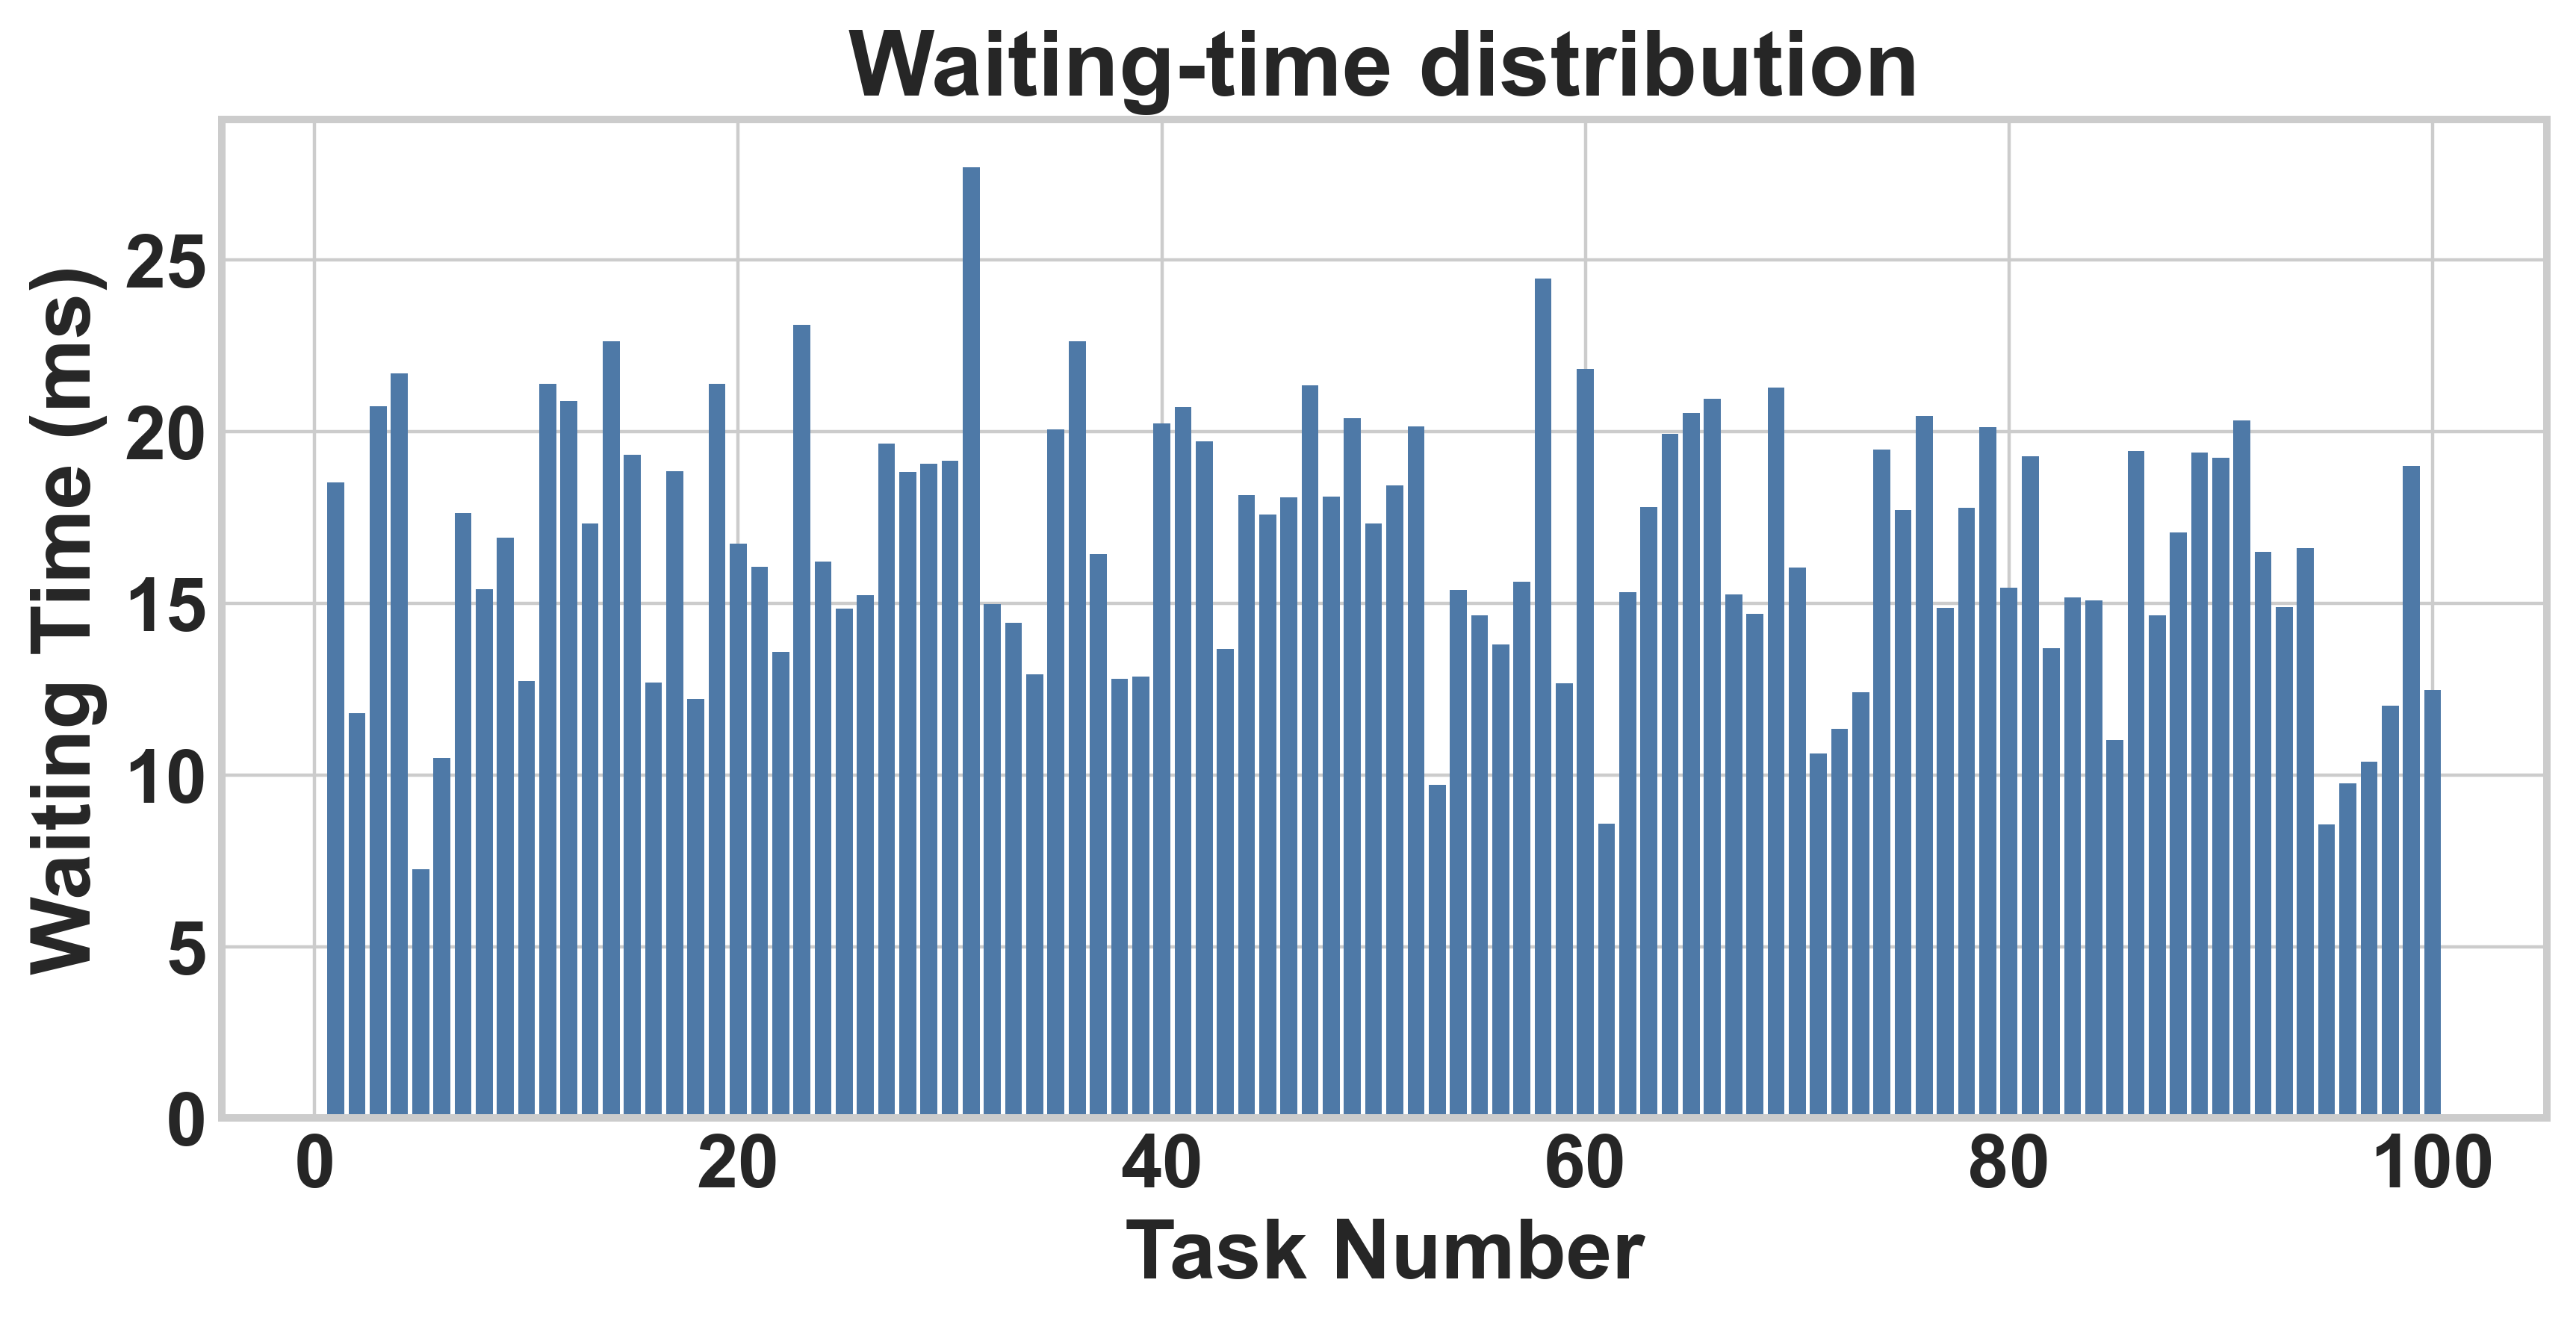
\includegraphics[width=\linewidth]{figures/s41598_final/fig17_case1_waiting_distribution.png}
\\[-0.2em]\textbf{(a)} Case distribution
\end{minipage}\hfill
\begin{minipage}[t]{0.32\linewidth}
\centering
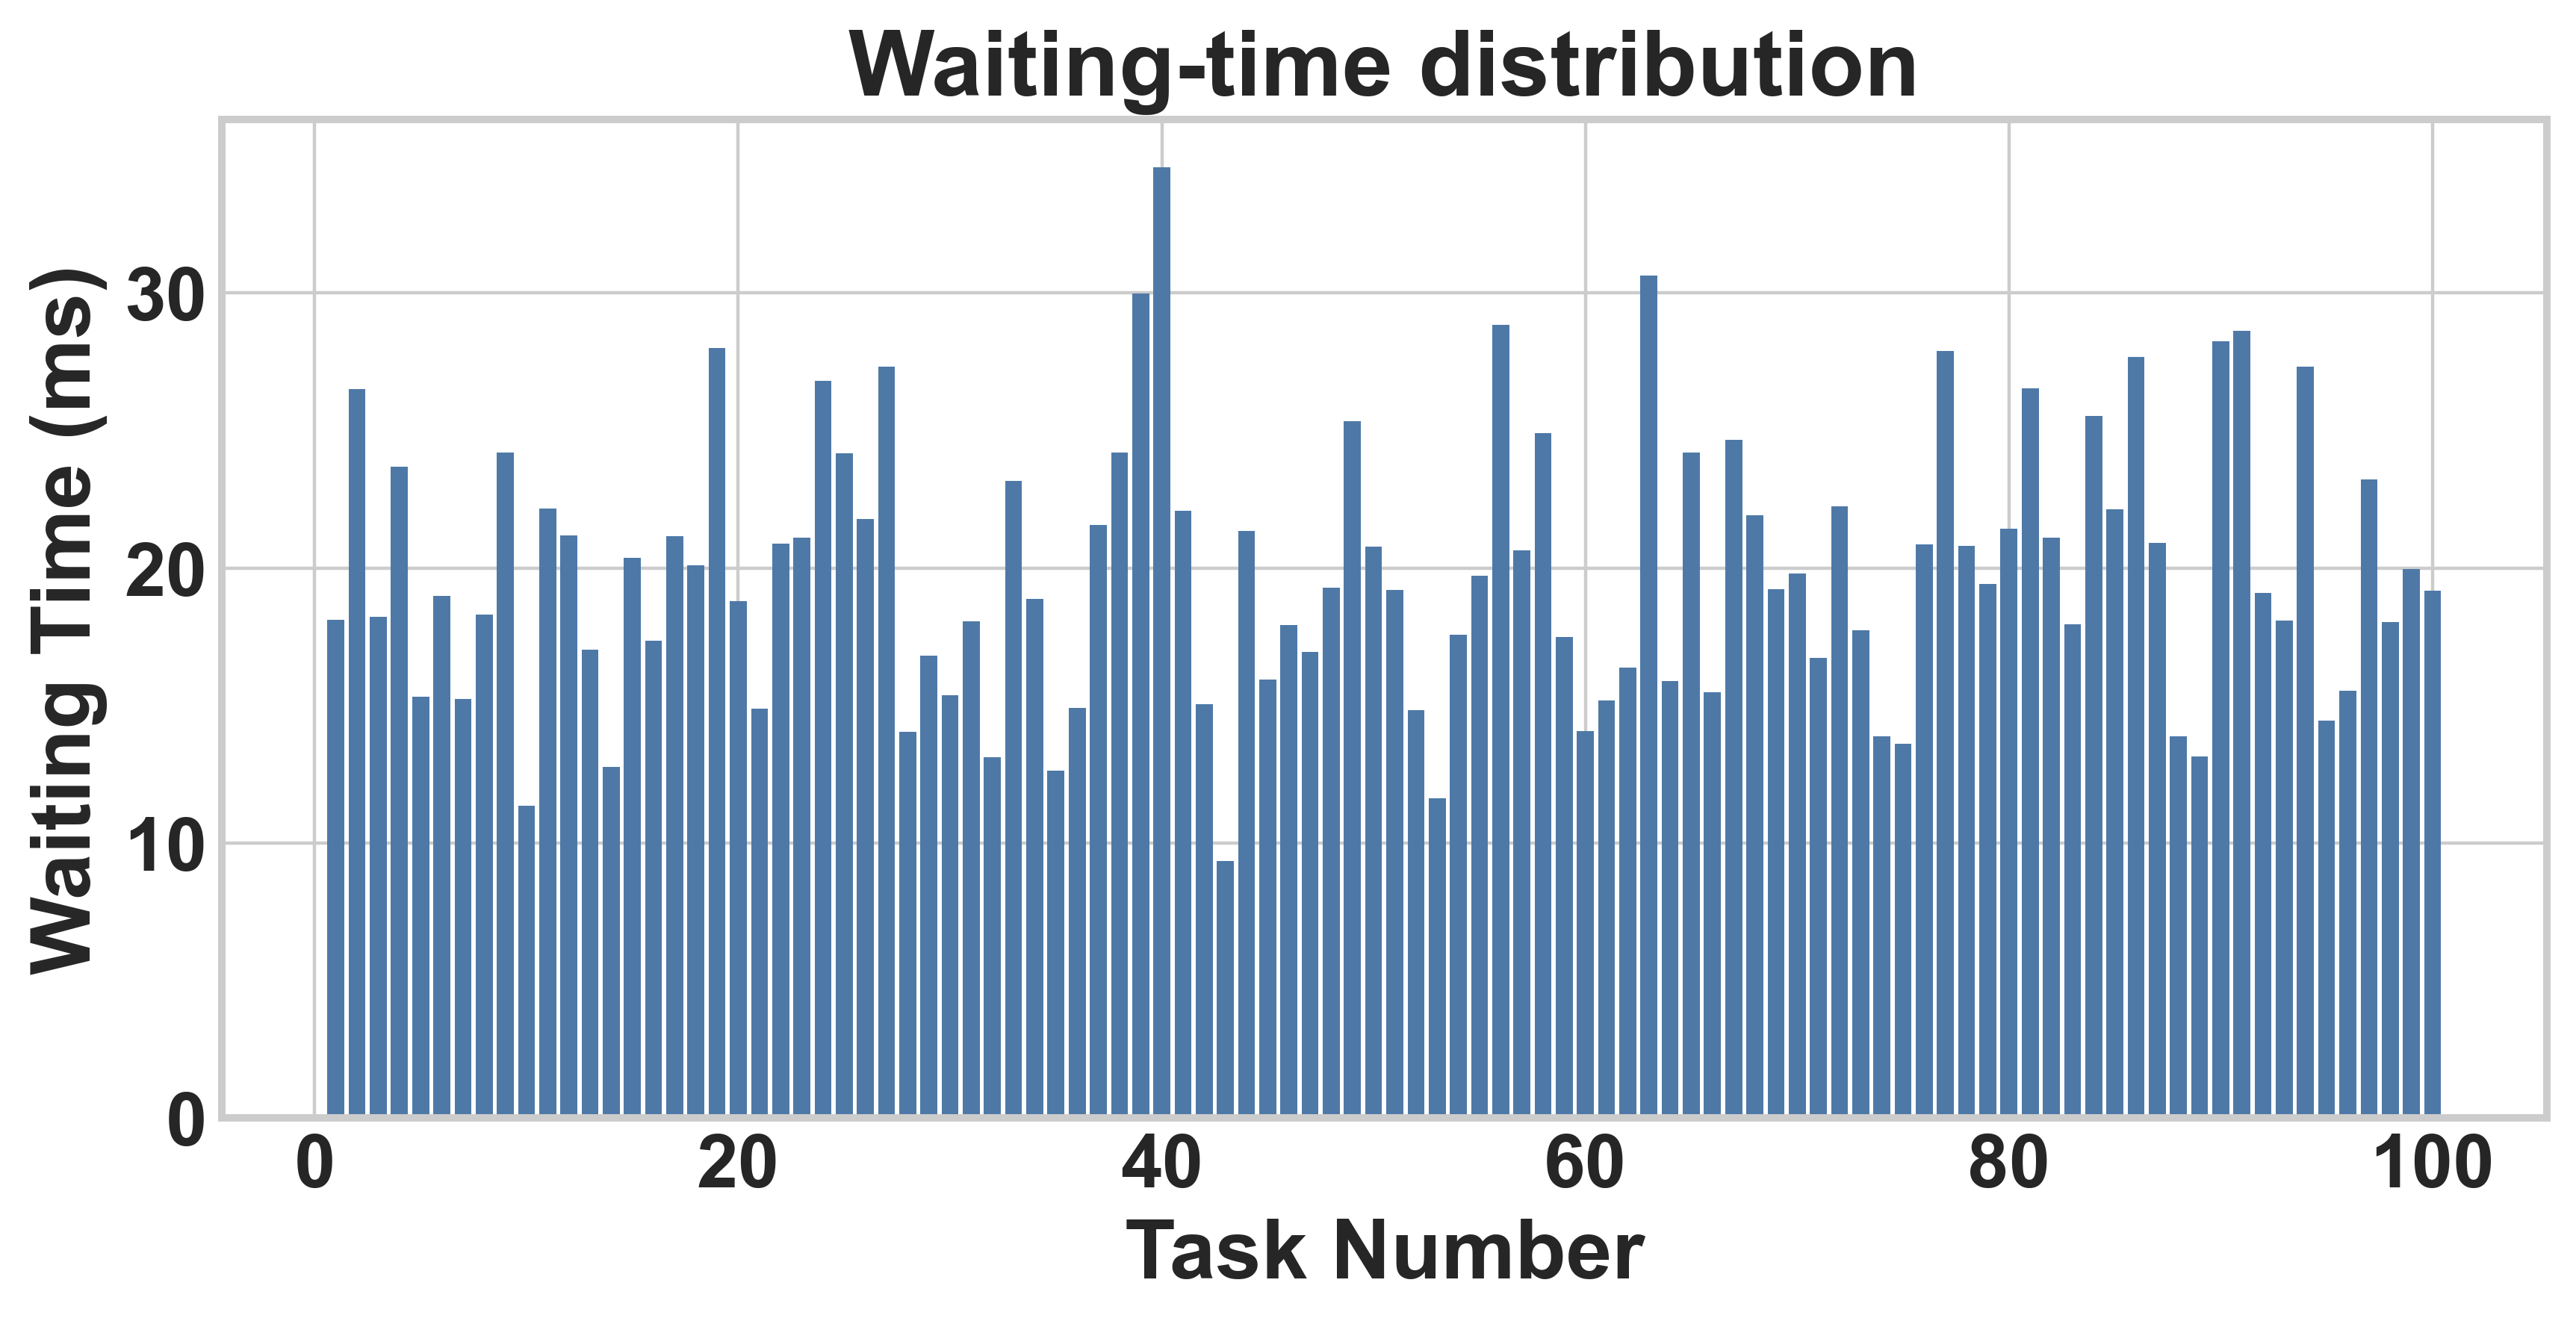
\includegraphics[width=\linewidth]{figures/s41598_final/fig18_case2_waiting_distribution.png}
\\[-0.2em]\textbf{(b)} Dynamic waiting
\end{minipage}\hfill
\begin{minipage}[t]{0.32\linewidth}
\centering
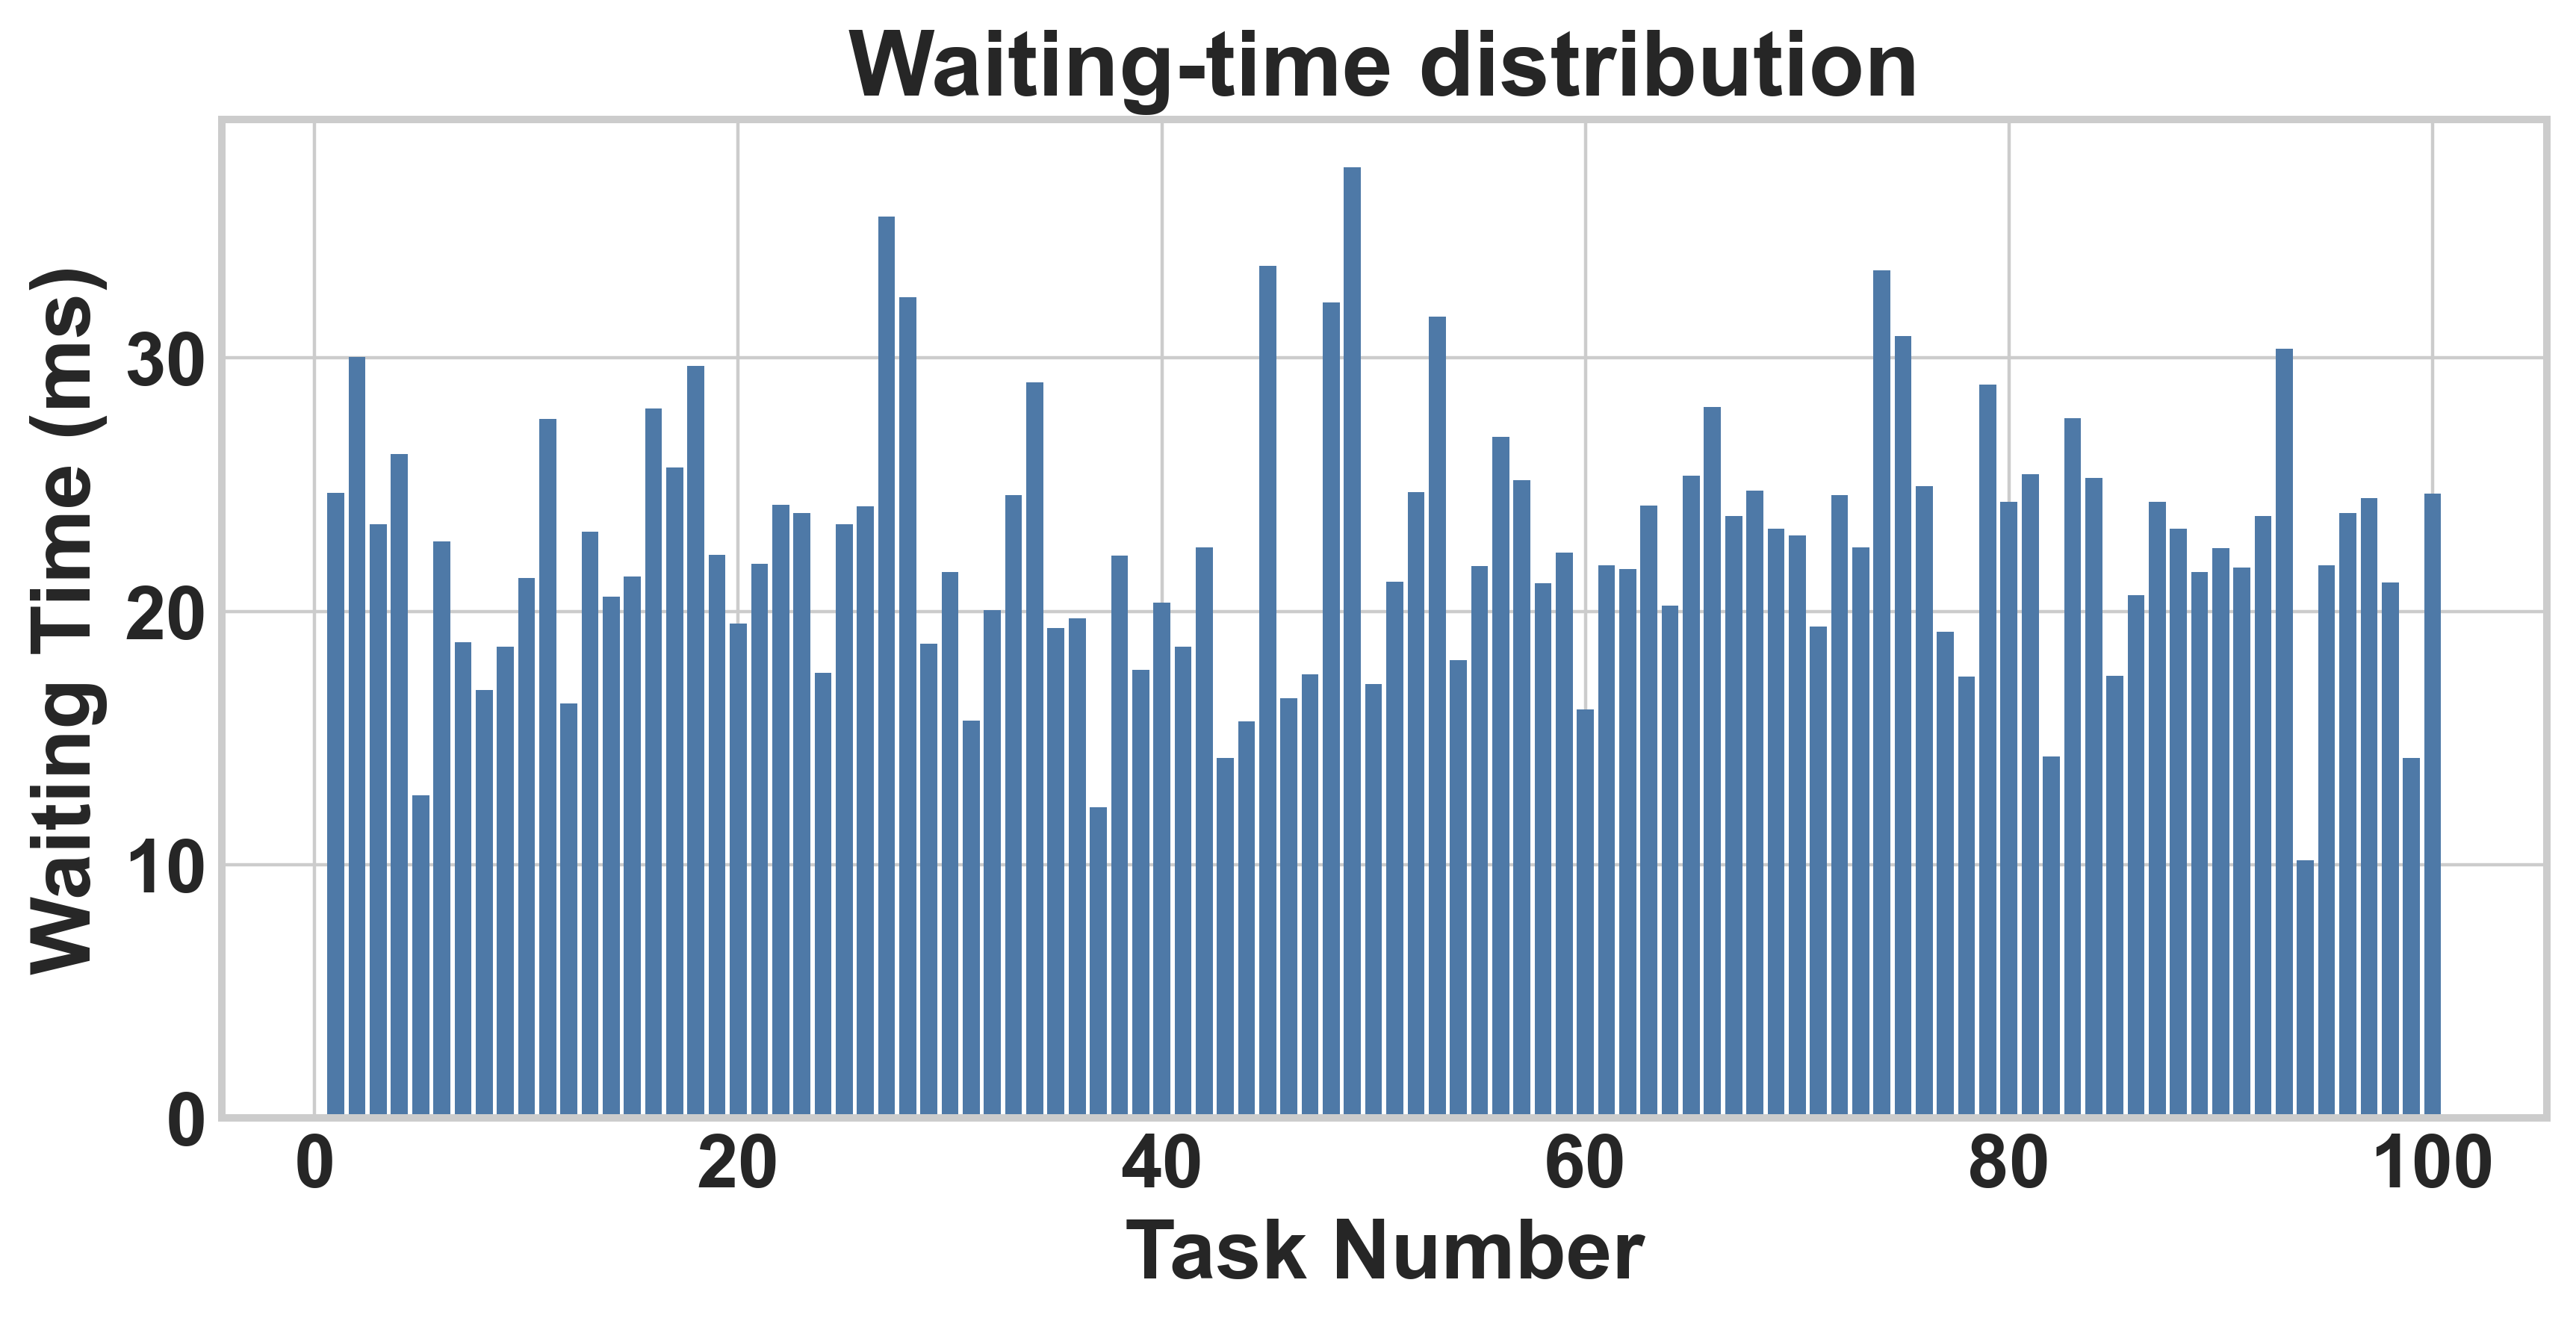
\includegraphics[width=\linewidth]{figures/s41598_final/fig19_case3_waiting_distribution.png}
\\[-0.2em]\textbf{(c)} Sensitivity alpha
\end{minipage}

\vspace{0.35em}

\begin{minipage}[t]{0.32\linewidth}
\centering
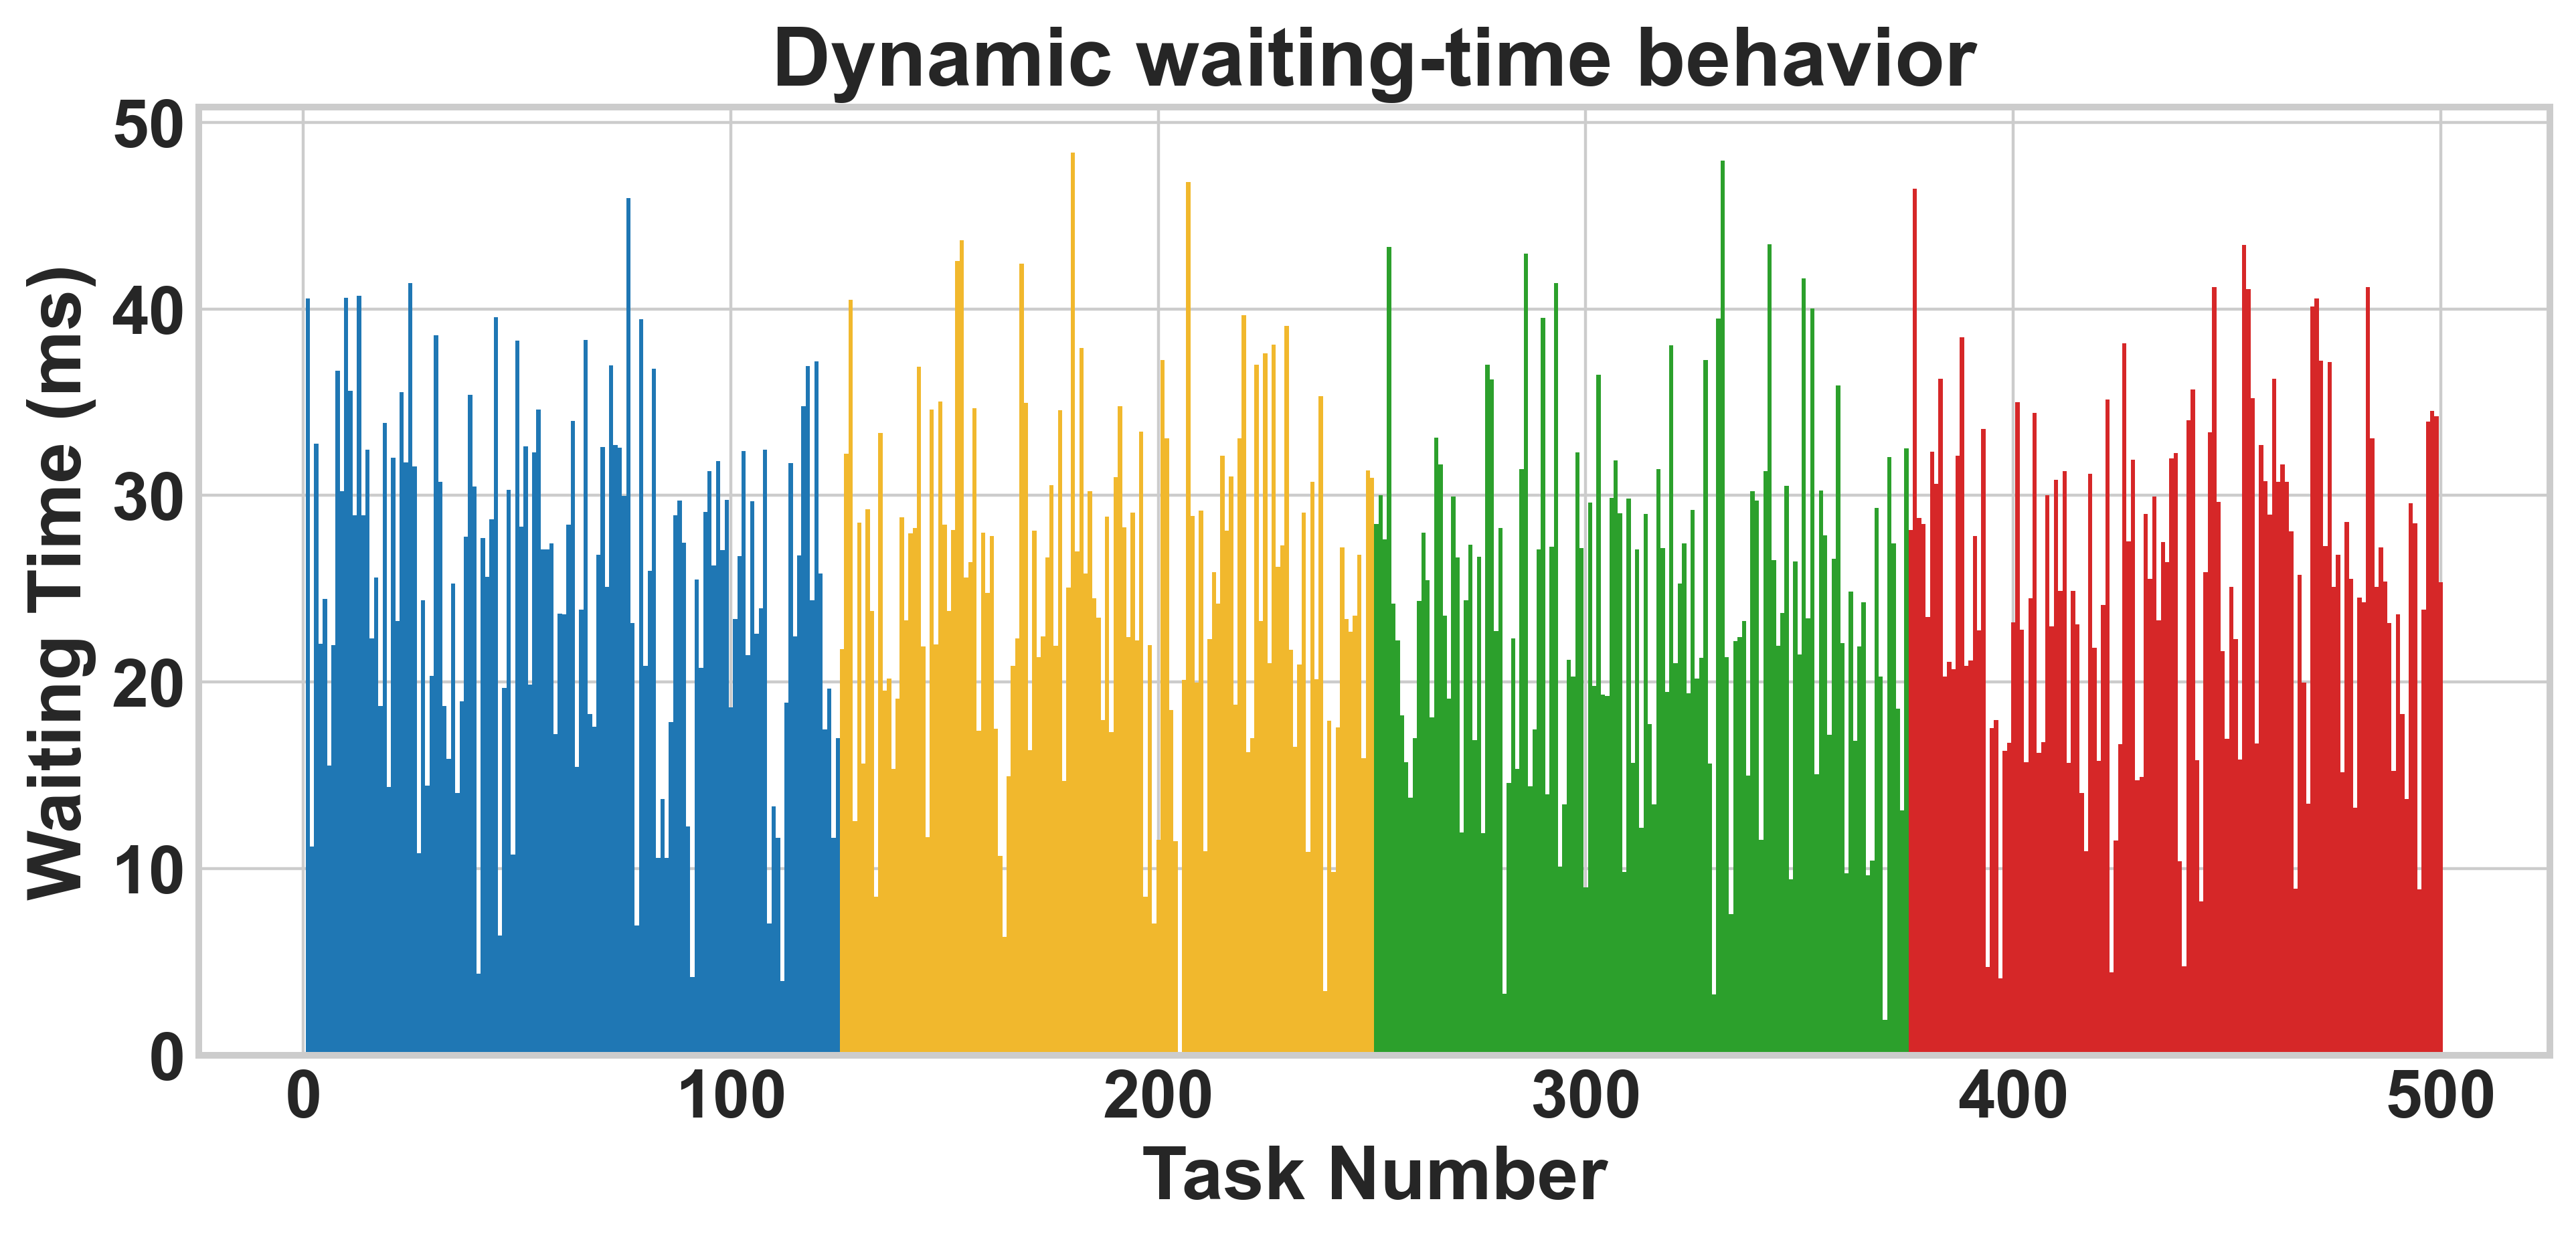
\includegraphics[width=\linewidth]{figures/s41598_final/fig20_dynamic_waiting_distribution.png}
\\[-0.2em]\textbf{(d)} Sensitivity beta
\end{minipage}\hfill
\begin{minipage}[t]{0.32\linewidth}
\centering
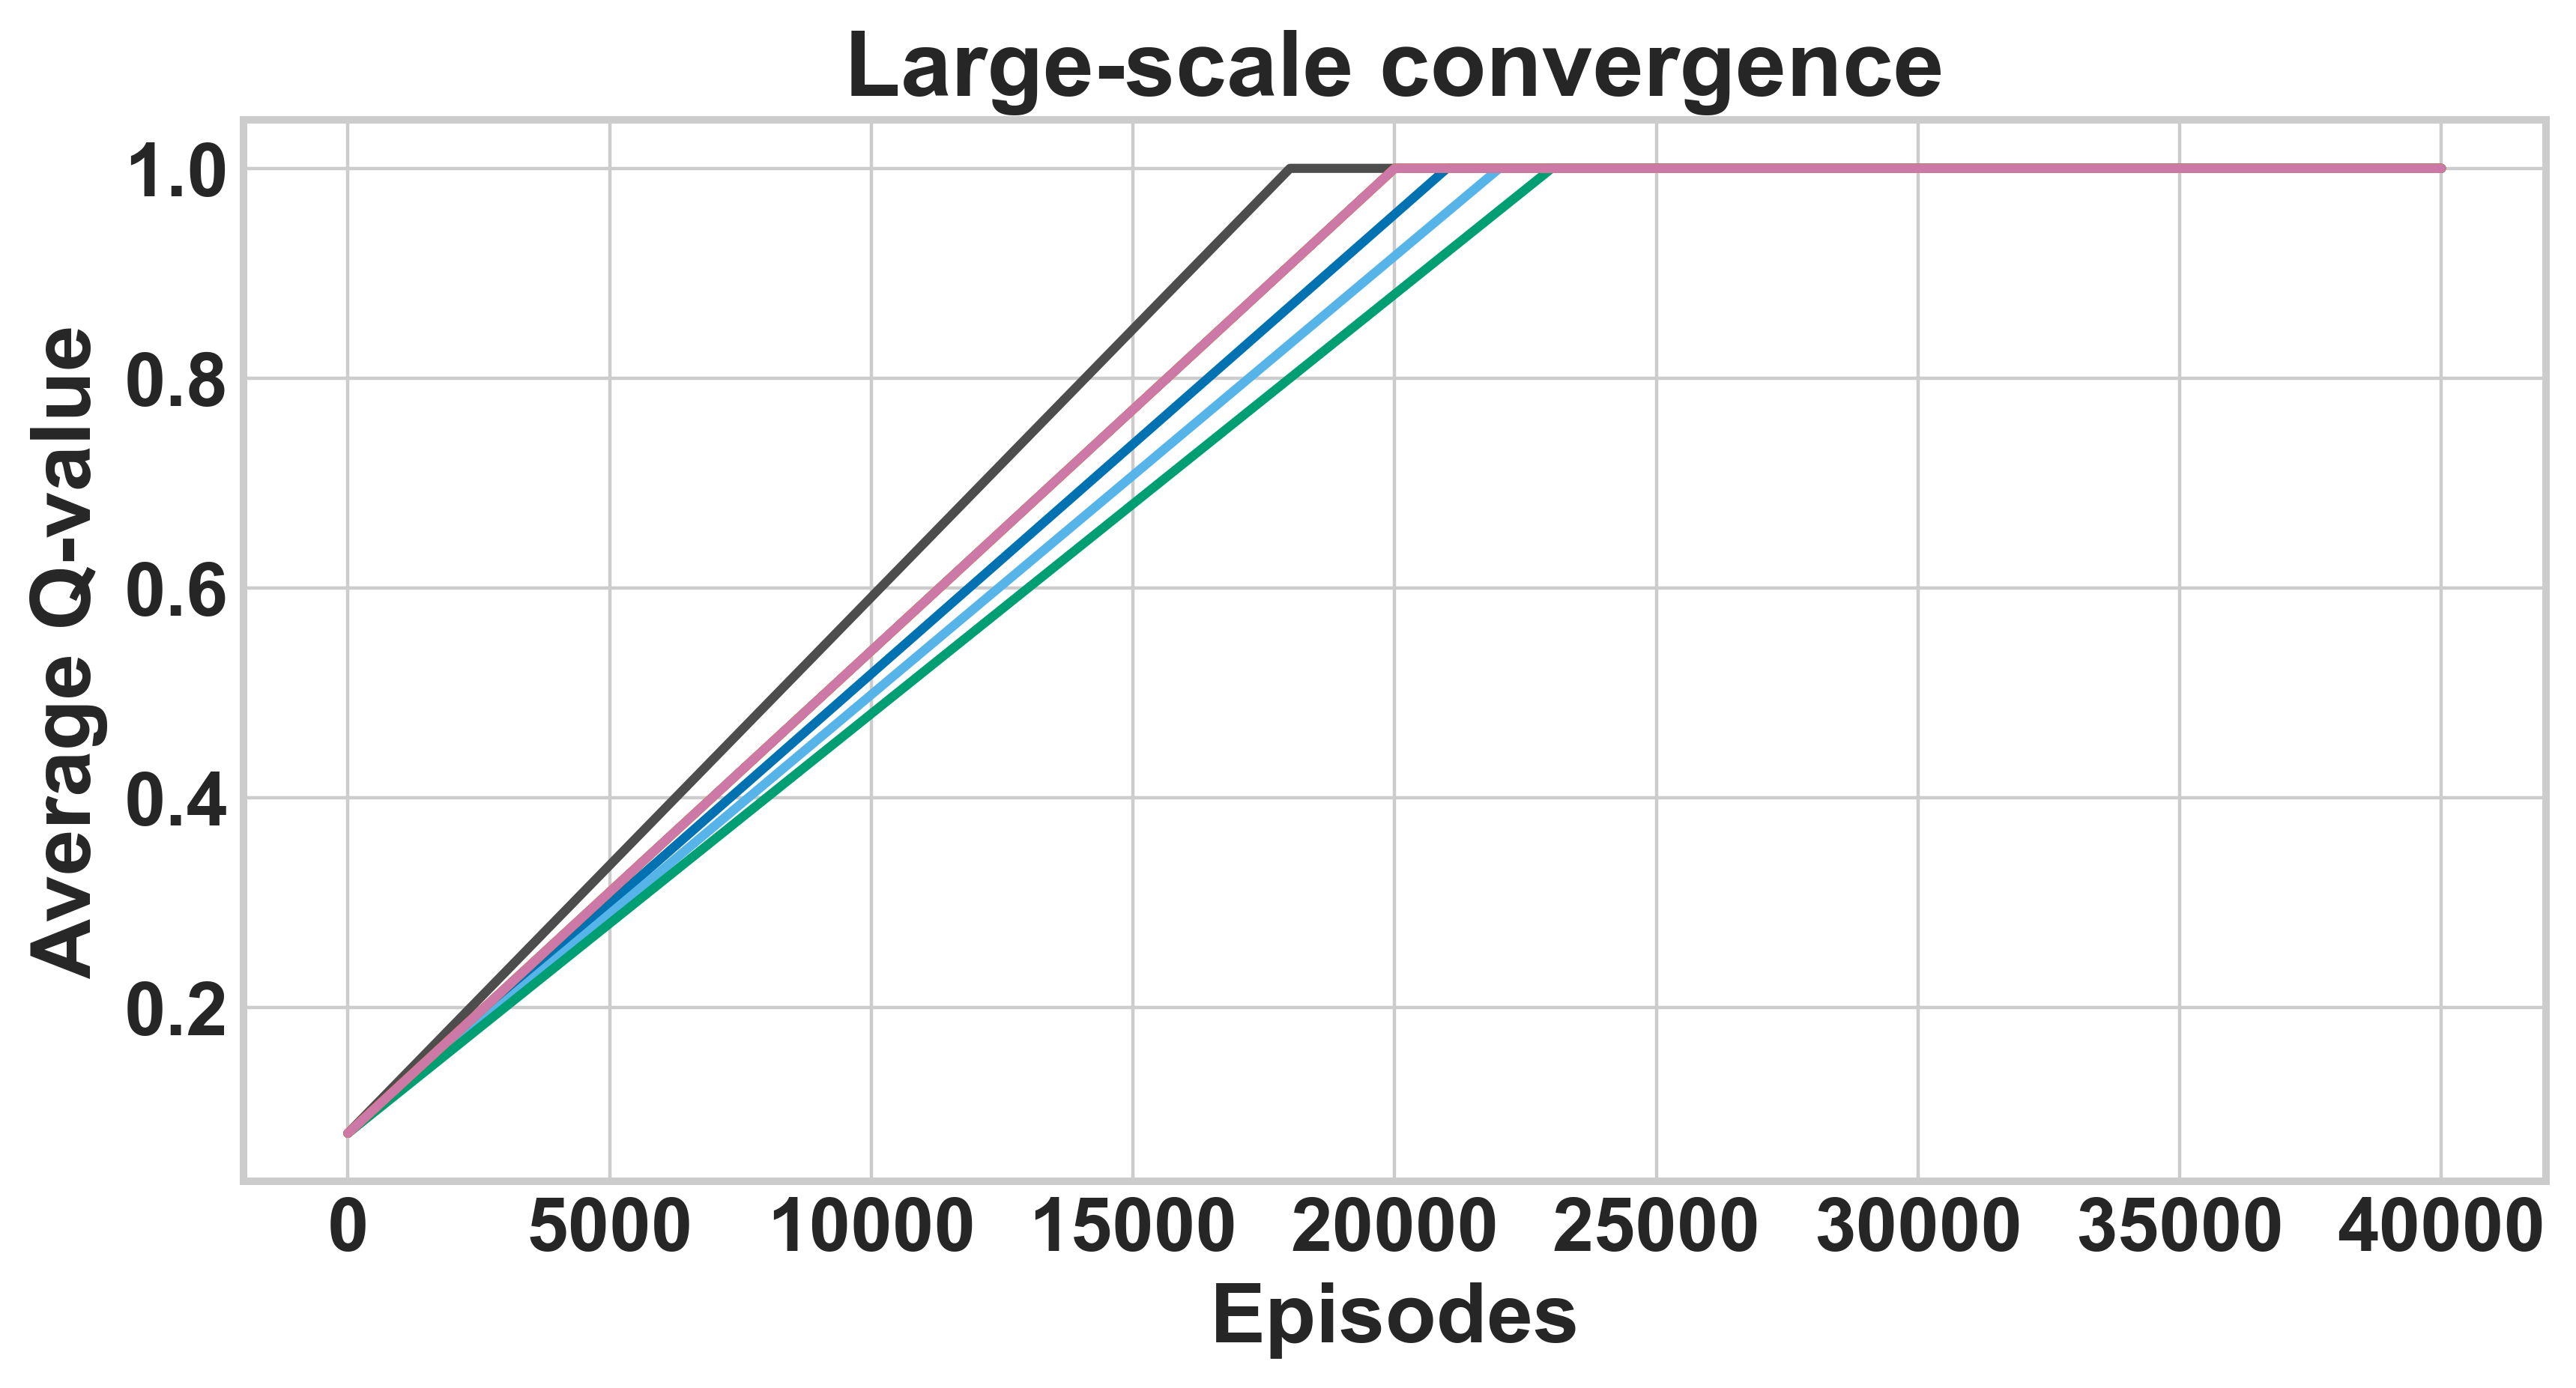
\includegraphics[width=\linewidth]{figures/s41598_final/fig23_large_scale_convergence.png}
\\[-0.2em]\textbf{(e)} Large-scale convergence
\end{minipage}
\caption{Supplementary Case-Oriented Results}
\label{fig:resD_supp}
\end{figure*}

\paragraph{Detailed supplementary interpretation}
Panel (a) reports case-distribution behavior across workload regimes and shows that AdaptiveSched variants remain comparatively stable as queue composition shifts from low-pressure to high-pressure slices. The hybrid policy maintains the most consistent cross-case profile, which is directionally aligned with the role-mixture objective of reducing regime-specific policy interference.

Panel (b) provides dynamic waiting trajectories and indicates that waiting-time growth remains lower and smoother for AdaptiveSched-Hybrid than for baseline policies under sustained queue pressure. AdaptiveSched-Base tracks the same trend but with a slightly larger waiting envelope, consistent with the interpretation that performative robustness helps stabilization while role-specialized routing improves fine-grained queue handling.

Panels (c) and (d) summarize sensitivity under controlled perturbations of shaping/optimization constants. The relative ranking is largely preserved across the tested range, while absolute metric values shift as expected with parameter variation. This supports robustness of comparative ordering without claiming full hyperparameter invariance.

Panel (e) documents the large-scale convergence trade-off discussed in the main text: one baseline can plateau earlier on a narrow convergence signal, whereas AdaptiveSched variants converge slightly later but achieve a better multi-objective operating profile on deadline, waiting, cost, and energy outcomes across the broader protocol.

\paragraph{Artifact availability}
All scripts used to generate the main and supplementary tables/figures are included under \texttt{benchmarks/}, including training/evaluation entry points, protocol-normalization logic, and inferential summary generation outputs. The public project repository is available at \url{https://github.com/Dhruv27Mishra/cloud}. For archival reproducibility, the submission package is prepared as a versioned release snapshot with a citable archive identifier to be provided in the camera-ready metadata; the current seed-level primary-metric outputs used for Table~\ref{tab:inferential_summary} are stored in \texttt{benchmarks/outputs/seed\_inferential\_final\_pipeline\_aligned/} for direct audit of paired comparisons.
\end{document}

